% Class:
\documentclass[notitlepage]{report}

% Fonts:
\usepackage[T1]{fontenc}
\usepackage{lmodern}

% Links:
\usepackage{hyperref}

% Maths:
\usepackage{amsmath}
\usepackage{amssymb}
\usepackage{mathrsfs,amsmath}
\newcommand{\e}[1]{\times 10^{#1}}
\usepackage{siunitx}

% Algorithms:
\usepackage{algorithm}
\usepackage{algpseudocode}

% Figures:
\usepackage{graphicx}
\usepackage{caption}
\usepackage{subcaption}
\graphicspath{ {./} }
\usepackage{float}

% Footnotes:
\usepackage[symbol]{footmisc}
\renewcommand{\thefootnote}{\fnsymbol{footnote}}

% Others:
\usepackage{pdfpages}
%\usepackage[backend=bibtex]{biblatex}
\usepackage{textcomp}
\usepackage{pdflscape}
\usepackage{titling}
\usepackage{tikz}
\usetikzlibrary{positioning, shapes.geometric}
\usepackage{listings}
\usepackage[toc,page]{appendix}

% Title:
\title{
	Sound-source Localisation using a Microphone-array for NUbots\\
	Final Report
}
\author{Mr. Clayton Carlon, C3327986\\Supervisor: Prof. Andrew Fleming}
\date{\today}

% Document:
\begin{document}

%\begin{titlepage}
\maketitle

\begin{figure}[H]
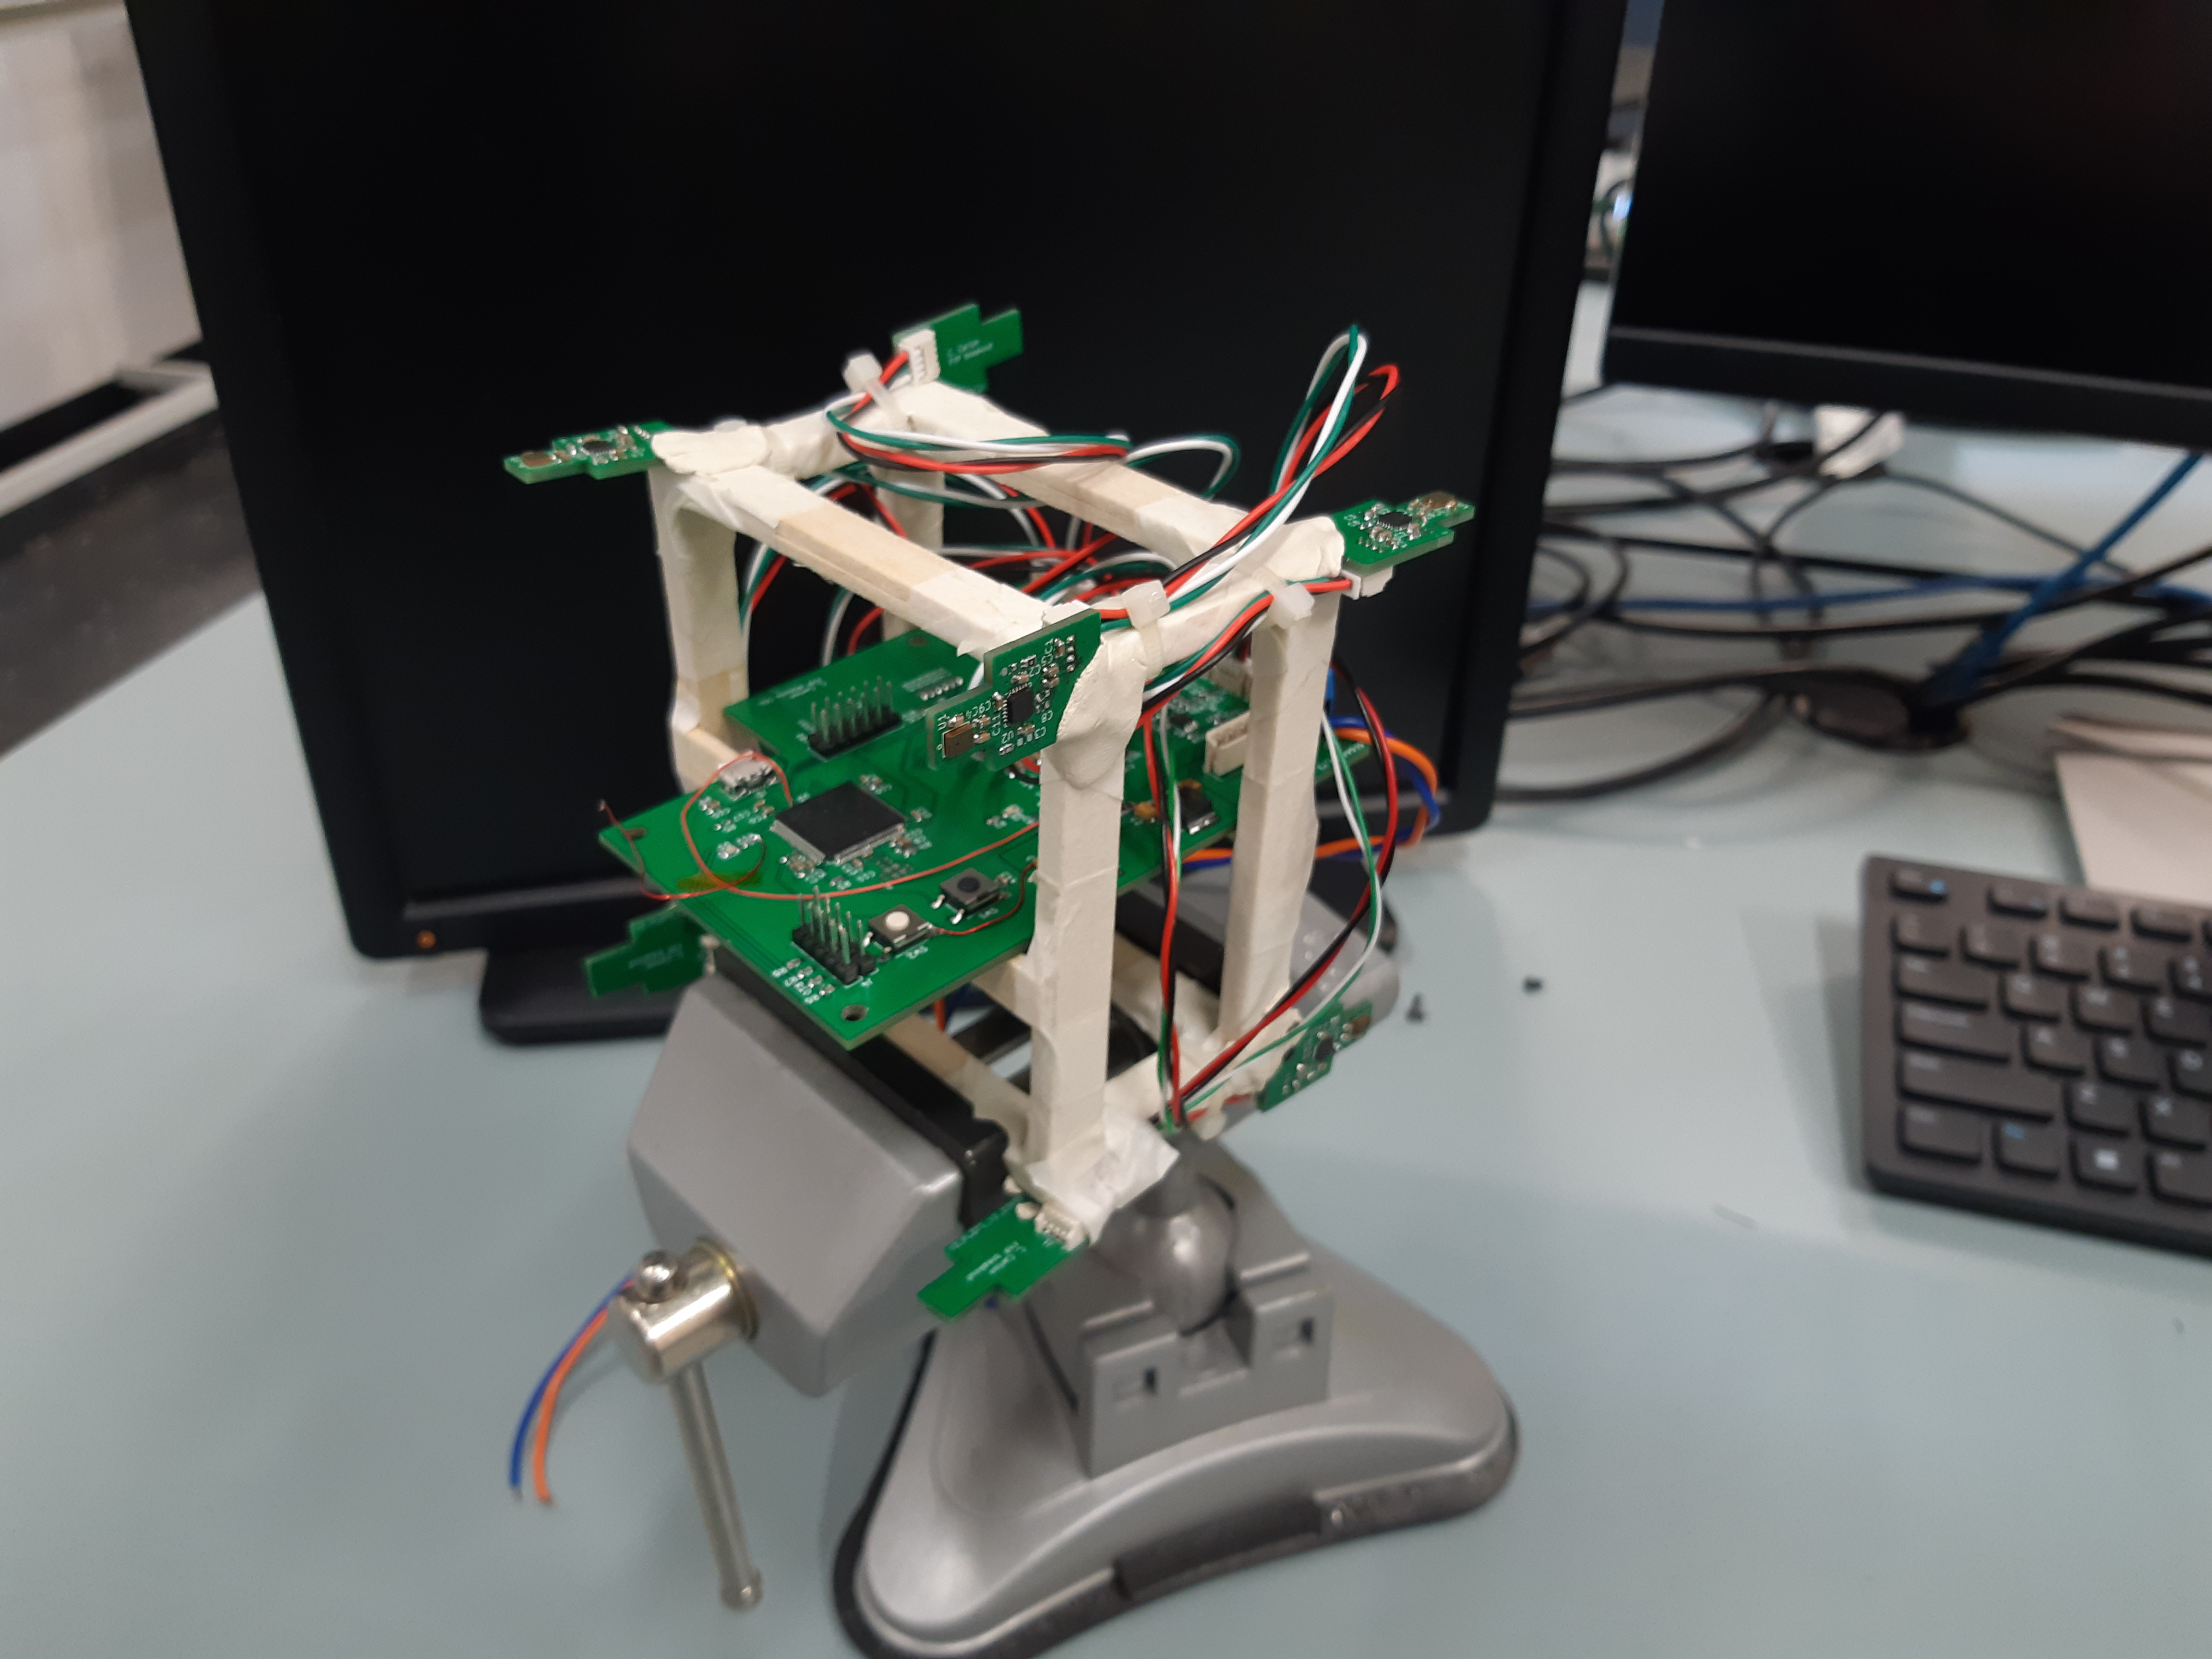
\includegraphics[width=0.75\textwidth]{./photo_array.jpg}
\centering
\end{figure}

\begin{abstract}
The ability to locate a source of sound is a highly wanted ability in robotics. This project was to design such a system on a lightweight embedded system with an array of microphones. A number of signal-processing techniques for such an array in the literature have been explored, two examples in which have been simulated. The chosen method was correlation-based beamforming also known as steered-response-power (SRP) which can estimated the three-dimensional direction of any sound with high enough signal-to-noise-ratio (SNR). Firstly, an algorithm was proposed and was tested again in simulation. Afterwards, a physical prototype was design and built along with firmware for the algorithm. Early results from the physical prototype have shown promising results although thorough physical experiments are still needed.
\end{abstract}
%\end{titlepage}

\section*{Acknowledgements}

I would like thank Prof. Andrew Fleming as my supervisor and the staff at the EE building for access to the soldering room. I would also like to thank the NUbots team for giving the initial inspiration and the support throughout.

\section*{List of Contributions}

This project has:
\begin{itemize}
	\item proved the concept and feasibility of sound-source-localisation on an embedded system,
	\item given an audio-platform for the NUbots team to use in the long term for future audio-related projects,
	\item given a localisation-technique on an embedded system for the NUbots team to use,
	\item and given inspiration for future revisions of the idea.
\end{itemize}

\tableofcontents

\chapter{Introduction}

Locating a source of sound is a long sought after ability in technology, especially in the study and development of robotics which seeks to emulate and compete with human senses. The main aspiration for this project is to develop an array of microphones along with an accompanying computation, preferably embedded, to locate a source of sound using signal-processing techniques. In the end, this system will be used on the football-playing robots in the NUbots team, the university's on-campus robotics team. Therefore, the problem for this project to solve was to develop a physical prototype along with a sound-source-localisation technique using a combination of electronics, embedded computing, and signal-processing so that the robots can locate events on the field and possibly interact with and selectively listen to humans.

\section{Background}

\subsection{NUbots}

NUbots \footnote{https://nubook.nubots.net/} is a multidisciplinary team under the University of Newcastle's robotics research group and has competed since 2002 in RoboCup, an international competition where humanoid robots play a simplified version of association-football\footnote{otherwise known as football or soccer}. The team is multidisciplinary and is made up of both undergraduate and postgraduate students in computer science and engineering. At this time, the robots on the team are modified versions of the igus\textregistered\ Humanoid Open Platform from Bonn University; this modified platform is called the NUgus\footnote{Hereafter will the specific robot be referred to as either the 'NUgus' or simply the 'robot'.} hardware platform and competes in the kid-size league.

\begin{figure}[H]
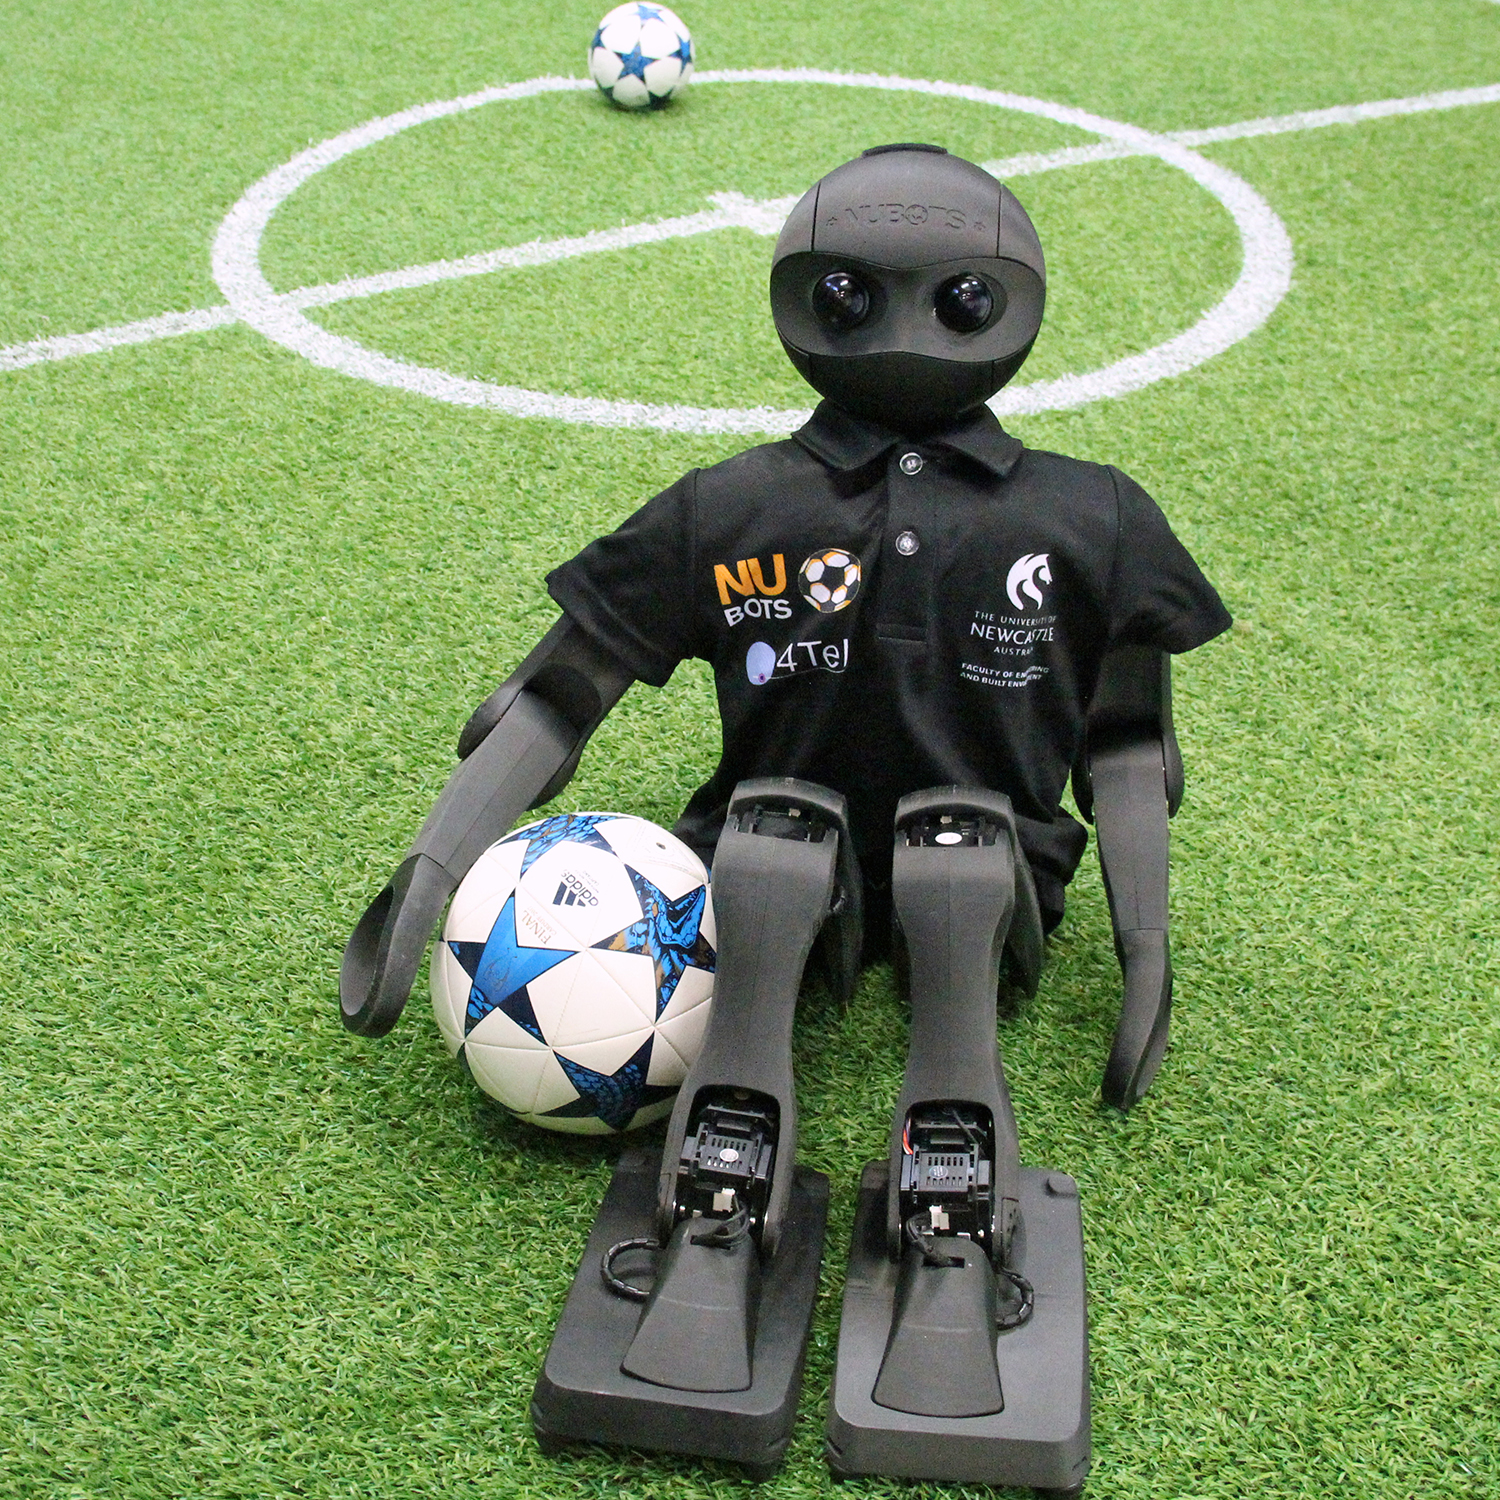
\includegraphics[width=0.9\textwidth]{./NUbot-sitting-down.jpg}
\centering
\caption{The NUgus robots are mainly used by the NUbots teams to compete in RoboCup}
\label{fig:nuguses}
\centering
\end{figure}

The remit of the team is broad and is not only competing in RoboCup. Although it strives to win this competition, the team also does research more generally in areas related to robotics, such as computer-vision, robotic locomotion and control, etc. Therefore, the project did not necessarily have to be tied to the said competition. Furthermore, this project, as it evolved, did not necessarily have to be used in the application of NUbots nor robotics more generally although the original idea came from NUbots. Sound-source-localisation is a broad area of study, and the final prototype can just as easily be employed in other applications, such as a video-conference-system, drones, etc.

\subsection{Applications}

Although this project is more a proof of concept, there are a number of useful long-term applications. One such is the localisation of a ball or a robot on the field. This system can be paired with a separate sound-classification system so that the robot can detect specific sounds and locate them. Another case is the ability for friendly robots on the same team to locate each other by giving deliberate bursts as beacons so to speak. A third application is the location of a whistle which human referees blow at the beginning of a game; to hear such a whistle may give a headstart over the other team.

However, this project was to develop a basic low-level prototype that will serve as a platform for furture-students on the team to develop such strategies and applications. In fact, the prototype could be used to stream audio-data through USB to the robot's computer for other systems such as speech-recognition.

Although sound-source-localisation will be helpful in a scenario of football-playing robots, the final system does not have to directly help the robot's performance in a match. The ability for a robot to interact with humans is a broad and well sought after goal. Even a basic demonstration of the robot turning its head towards a human speaker can help the team's outreach and marketing in exhibition-shows, publicity-events, etc. Not only will this help sponsors and thus funding for the team, but even the basic proof of concept also contributes further to the team's research in and remit of robotics.

\section{Scope}

It has been found in the first part of the project that the literature lacked many examples actually applying a physical and lightweight. Many examples have the system running on a laptop or even a desktop. Therefore, the main area of the project was not so much to reinvent a new technique of sound-source-localisation but rather to take an existing and well-established technique and apply it to an embedded application where there are far more constraints such as computation.

Thus, the scope deals with both the research of techniques and the design of the electronics and the firmware. The novelty comes from the design, although there is one new minor improvement to the algorithm, see Section-\ref{Confidence}.

Ideally, the project should have yielded a working prototype fitted on one of the NUgus robots. At the beginning, since the project was more intended as a proof-of-concept, its goals were thus somewhat open-ended. However, such basic goals were that it should at the very least:
\begin{itemize}
	\item estimate the three-dimensional direction, i.e. the azimuth and the elevation,
	\item locate a reasonably distinct sound in a moderate environment, e.g. a whistle, a lone voice, a loud thud,
	\item and handle the noise from the motors of the robot which will be nearby.
\end{itemize}
Further goals were that it can:
\begin{itemize}
	\item estimate the distance along with direction, essentially locate the source's full coordinates in three-dimensions,
	\item track the location over time using e.g. a Kalman filter,
	\item locate multiple simultaneous sources, as long as they have relatively distinct locations,
	\item spatially filter the localised sound,
	\item and work well enough in noisy and reverberant environments, e.g. in a hall full of people.
\end{itemize}

% accuracy 

\chapter{Literature-Review and Theory}

In order to understand how one would localise a sound, exisiting examples in the literature must be researched to gain inspiration and knowledge. This section mostly looks at the broad areas and some chosen examples. Furthermore, since this literature-review is heavily coupled with the theory, the latter is also discussed here. 

Since sound-source-localisation is a much widely researched problem, in e.g. robotics, drones, video-conferencing, the military, submarines, hearing aids, etc., the review of the literature can be quite broad. To narrow the search, and to also find examples that are most relevant to this project, especially for computation and dimensions, this review has mostly considered literature with a robotics context, rather than a large-scale military outdoor application for example. Indeed, sound-source-localisation for drones shares a good deal with that for robotics, e.g. the influence of motors, but one important difference is the fact that applications for drones are mostly outdoors rather than indoors where the reverberation is an important factor.

To further help narrow the scope of the search, most methods considered are ones that use an array of at least three microphones and use some kind of classical signal-processing. Other kinds of methods exist such as binaural approaches with two microphones and head-models \cite{argentieri_survey_2015} and those that use machine-learning, such as convolutional neural networks \cite{sakavicius_multiple_2022}. It is not necessarily that these other approaches will be ignored outright but rather that the scope of the literature-review as well as the project as a whole will be kept relevant in order to ease the search and to deepen the study of a few relevant methods.

\section{Overview of Methods}

There are already a few reviews of the literature, each going through a number of existing and studied methods for sound-source-localisation. A survey \cite{argentieri_survey_2015} attempted to give a state of the art of sound-localisation in robotics. It dealt with two main areas, namely binaural approaches and array-based approaches. Since an array of microphones will be used in this project, the latter area is most relevant. All the approaches of which that the survey explored were listed as such:
\begin{itemize}
	\item MUSIC,
	\item time-difference of arrival (TDOA), and
	\item beamforming.
\end{itemize}

Some of the methods and approaches reviewed hereafter are only described on the surface, but some hand-picked ones are further studied in the next chapter on simulation.

\section{The far Field and the near Field} \label{The_far_Field_and_the_near_Field}

One important distinction about the geometry is the far field and the near field. Many methods approximate their algorithm and computation by assuming that the source is in the far field where the distance between the source and the array is comparably longer than the array's width. This is such that the sound-waves may be assumed to be planar at the array and such that the direct lines between the source and each microphone may be assumed to be parallel. 

Some methods, especially those of beam-forming, can estimate distance but only in the near field where the distance between the source and the array is comparable to the array's width. However, since the microphone-arrays in robotic applications are generally small, only the far field is an acceptable assumption. This may especially be the case for NUbots where candidate space for an array on the existing NUgus is sparse, and a smaller array may have to be chosen. Thus, one must keep this distinction in geometry in mind hereafter.

\section{Time-Difference of Arrival} \label{Time_Difference_of_Arrival}

A simple yet proven way to estimate the DOA of a sound-source using a microphone-array is to calculate the difference in time \cite{argentieri_survey_2015}. Commonly, the TDOA of two microphones is often found by the cross-correlation of two signals, the highest peak of which corresponds to the estimated TDOA. The cross-correlation is generally written in discrete-time as:
\begin{equation}
R_{ij}(\tau) = \sum_{n=0}^{N-1} x_i[n]x_j[n-\tau]
\end{equation}
where $x_i$ and $x_j$ are the two signals, from two microphones for example. Cross-correlation is useful in particular because it has an equivalent calculation in the frequency-domain:
\begin{equation}
R_{ij}(\tau) = \mathfrak{F}^{-1} \left( X_i[k]X_j[k]^* \right)
\end{equation}
where $X_i[k]$ and $X_j[k]$ are the Fourier transforms of $x_i$ and $x_j$ respectively. Unlike the original calculation which relies on addition and has a complexity of $O(N^2)$, this frequency-domain equivalent relies on multiplication, can be made more efficient by FFT, and has a complexity of $O\left(N\ln(N)\right)$ \cite{valin_robust_2003}.

An advanced form of this TDOA estimation is the generalised cross-correlation (GCC):
\begin{equation}
R^{(w)}_{ij}(\tau) = \mathfrak{F}^{-1} \left( \psi[k]X_i[k]X_j[k]^* \right)
\end{equation}
where $\psi[k]$ is the spectral weighting \cite{argentieri_survey_2015}, \cite{rascon_localization_2017}. A common weighting is the phase-transform (GCC-PHAT):
\begin{equation}
\psi[k] = \frac{1}{\lvert X_i[k] \rvert \lvert X_j[k] \rvert}
\end{equation}
which whitens the signals and emphasises only information on the phases rather than the magnitudes.

The TDOA can therefore be estimated as the point in time where the GCC-PHAT is highest:
\begin{equation}
\Delta t_{ij} = \text{argmax}_\tau \left( R^{(w)}_{ij} (\tau) \right)
\end{equation}

Given the TDOA $\Delta t_{ij}$, and assuming that the source is far enough, the two-dimensional angle of arrival at a pair of microphones can be estimated from simple trigonometry of parallel lines:
\begin{equation}
\theta = \sin\left( \frac{c\Delta t_{ij}}{d_{ij}} \right)
\end{equation}
where $c$ is the speed of sound, and $d_{ij}$ is the displacement between the microphones, and assuming that the source is in the far field.

The former expression is the most basic approach for a simple two-dimensional estimation of a single angle, often the azimuth. There are of course more sophisticated examples of finding the source three-dimensionally, even with distance.

\subsection{Distance}

The estimation of distance is not very common in TDOA-based methods. Most examples only localise the direction, whether it is two-dimensional or three-dimensional. As said before, the TDOA yields a hyperbola or hyperboloid as the locus of the source. Therefore, a naive method would be to find the intersection given at least two pairs of microphones. However, error and noise of course make this hard as well as the computation in a robotics context \cite{rascon_localization_2017}.

Another way is to use two or more sub-arrays that yield single DOAs and are used to triangulate on a position \cite{rascon_localization_2017}. However, such a method would need sub-arrays that are far apart enough which is hard for a small robot where space is a luxury.

\subsection{Reverberation}

Reverberation is a big influence on the estimation of the TDOA, especially in a room, since it leads to delayed reflections of the signal which show up in the GCC-PHAT. A statistical analysis \cite{gustafsson_source_2003} showed that the PHAT is the best estimator for the TDOA. The numerical examples in the paper showed good results as long as the reverberation-time was more than 0.07 \si{s}, the displacement between the microphones is longer than 0.2 \si{m}, and the distance between the source and the microphones is longer than 1.5 to 2 \si{m}. The same examples also showed that the probability of outliers was "tolerable" for a SRR more than 0 \si{dB}.

Another analysis \cite{brandstein_robust_1997} simulated three methods of estimating the TDOA, namely GCC-PHAT, GCC-ML, and Biweight. For all three, both the percentage of anomalies and the RMS error worsened for a reverberation-time longer than 0.1 \si{s}.

However, although GCC-PHAT generally handles reverberation well, it does not handle noise well across the spectrum since the algorithm gives all frequencies equal weight \cite{valin_robust_2003}. It especially does not do well with narrowband signals such as tones or voice which take up a small section of the spectrum.

\subsection{Multiple Sources}

Although the localisation of multiple sources has been explored for other methods such as beam-forming, it has not been explored much in TDOA-based methods. This is since most examples in the literature have been built on top of the basic idea of a single peak in the GCC-PHAT. However, the relationship between secondary peaks in the cross-correlation and other sources has been discussed.

Only a few basic studies in the fundamental relationship were done. A convention paper \cite{clifford_calculating_2010} proposed a method in the context of audio-engineering where multiple sources manifested themselves as distinct peaks in the GCC-PHAT. The results showed an accuracy of at least 85 \% where the SNR is at least 46.5 \si{dB}. However, the paper only considered the estimation of the TDOA in the context of musical instruments, not localisation, and the experiment was performed with little reverberation in mind. Another analysis \cite{kwon_analysis_2010} derived the mathematical cross-correlation function based on GCC-PHAT for multiple sources but did not seem to give much experimental data. 

Even so, no literature examples were found that exploited this relationship of secondary peaks for localisation in robotics \cite{rascon_localization_2017}. However, some studies have lately developed algorithms albeit not in a robotics context. A paper \cite{brutti_multiple_2010} proposed a method where an acoustic map, such as GCF or SRP-PHAT, is used to find the most dominant source which is then de-emphasised by lessening the GCC-PHAT at the time-delay corresponding to that source; this is repeated for the next most dominant source until all others are located. However, the paper only tested this method for the near field.

Another paper \cite{boora_tdoa-based_2020} proposed a method of a delay density map made up of cubic subvolumes each of which weighted by a likelihood that a source is in it. The tested system had a resolution of 0.2 \si{m} and an RMS error at worst of about 0.6 \si{m} at an SNR of 5 \si{dB}. The experiments were tested for both the near field and the far field as well as for different arrays. The reverberation-times at 60 \si{dB} in such experiments were tested from 0.11 to 0.55 \si{s}. It also compared its own method with that of GCF-D (GCF De-emphasised) where theirs performed better.

Even given a method that only locates a single source at a time, one other way to find multiple sources is to cluster multiple estimated DOAs over many time-windows or frames. One paper \cite{rascon_lightweight_2015} does such by tracking sources with a threshold on angle and smoothing such tracking with a Kalman filter. An adaptive variation of the K-mean++ algorithm has also been used to cluster multiple sources in an aforesaid paper \cite{hu_estimation_2009}.

\subsection{Literature Examples}

\subsubsection{Valin et al., 2003, Robust Sound Source Localization Using a Microphone Array on a Mobile Robot}

One method \cite{valin_robust_2003} solves a set of simultaneous equations from at least five microphones using the pseudo-inverse of a matrix; this yields a vector giving the three-dimensional direction. It also uses a different weighting than GCC-PHAT which gives more weight to areas of the spectrum where the SNR is higher. 

The experiment was performed with eight microphones in an open rectangular prism ($0.5\times 0.4\times 0.36$ \si{m}) on top of a mobile robot as seen in Figure-\ref{fig:valin_2003_robot} "in a room with a relatively high noise level mostly due to several fans in proximity" with "moderate" reverberation. The computation was done on a desktop PC and used about 15\% of the CPU. Three sounds were tested, speech, snap of fingers, and tap of boot. The results showed an estimated direction that degraded as the source got nearer to the array as seen in Figure-\ref{fig:valin_2003_plot}; the mean-square-error was at best 0.6 and at worst 4.9 \si{\degree} with the distance being from 0.3 to 5 \si{m}. This degradation was most likely because of the far-field assumption. The system works "properly" between 3 and 5 \si{m} although the authors claimed this as a result of "the noise and reverberation conditions". They also said that broadband signals were detected better than narrowband ones like tones.

\begin{figure}[H]
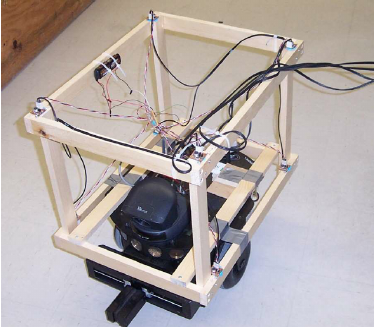
\includegraphics[width=0.75\textwidth]{./valin_2003/robot.png}
\centering
\caption{The microphone array on top of the mobile robot in \cite{valin_robust_2003}}
\label{fig:valin_2003_robot}
\centering
\end{figure}

\begin{figure}[H]
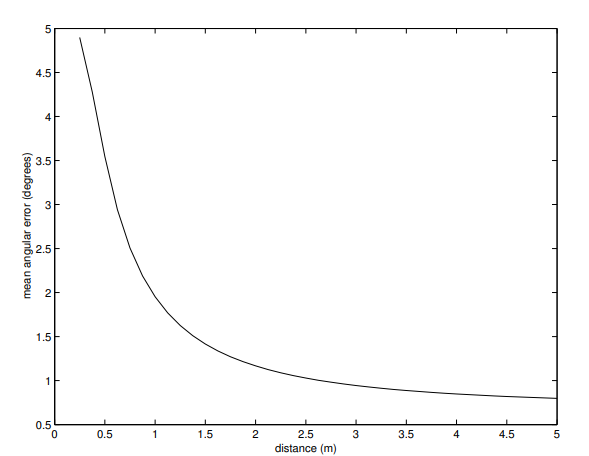
\includegraphics[width=0.75\textwidth]{./valin_2003/plot.png}
\centering
\caption{The mean angular error as a function of the distance between the source and the array in \cite{valin_robust_2003}}
\label{fig:valin_2003_plot}
\centering
\end{figure}

\subsubsection{Chen \& Xu, 2019, A Sound Source Localization Device Based on Rectangular Pyramid Structure for Mobile Robot}

However, the former method only computes the bearing, at least for the far field which is more relevant for the case with a smaller array. Another example \cite{chen_sound_2019} estimates the full three-dimensional coordinates of the source by an iterative algorithm based on Newton's method to solve a set of spatial coordinate-relations. This example also had a few improvements such as a partitioning process, a fast search-strategy of the GCC peak, a screening strategy, and a new weighting function in the GCC that dealt with reverberation. However, this proposed weighting function needed beforehand the parameters of the environment and the rough displacement of the source; the authors have admitted that this limits the universality. In simulations, the improved weighting function gave a better distinct peak in the GCC for a reverberation-time of 300 \si{ms}. 

This method was tried on an array of five microphones forming a rectangular pyramid 0.25 \si{m} wide and 0.125 \si{m} tall as seen in Figure-\ref{fig:chen_2019_array}. The performance was tested at different points around the array from 1 to 6 \si{m} and with a SNR of 45 \si{dB}. The error in distance increased as the source was further away; this was observed at best as 0.05 \si{m} and at worst as 0.25 \si{m}. The error in azimuth varied little in both distance and bearing and was observed as being within 1.5 \si{\degree}. The performance was also tested at different levels of SNR, from 40 to 10 \si{dB}. In the worst case of 10 \si{dB}, the error in distance was observed at worst as 0.4 \si{m} seen in Figure-\ref{fig:chen_2019_distance_SNR}. The paper neglected any evaluation of the estimated elevation, considering that the geometry of the array is not symmetrical. Furthermore, the computational needs were not discussed in depth.

\begin{figure}[H]
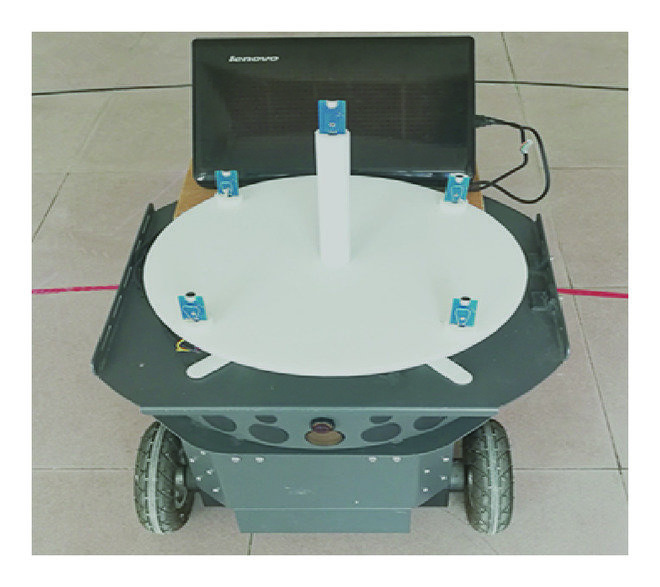
\includegraphics[width=0.75\textwidth]{./chen_2019/array.jpg}
\centering
\caption{The microphone array in \cite{chen_sound_2019}}
\label{fig:chen_2019_array}
\centering
\end{figure}

\begin{figure}[H]
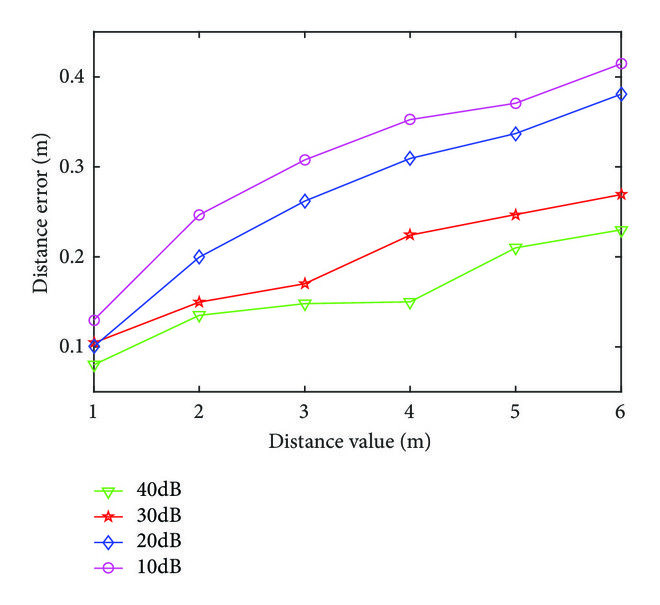
\includegraphics[width=0.75\textwidth]{./chen_2019/distance_SNR.jpg}
\centering
\caption{The error in distance as a function of distance for different SNRs in \cite{chen_sound_2019}}
\label{fig:chen_2019_distance_SNR}
\centering
\end{figure}

\subsubsection{Manamperi et al., 2022, Drone Audition: Sound Source Localization Using On-Board Microphones}

Potential unwanted noise from servo-motors, etc., may affect and disrupt how well the system localises wanted sources. A very recent study \cite{manamperi_drone_2022} set out an approach that estimated the azimuth and elevation and mitigated the noise from a drone's motors. Here, the authors computed the GCC-PHAT as an angular spectrum for many pairs of microphones and summed each pair's angular spectra; this method is similar to SRP-PHAT in that the azimuth and the elevation corresponding to the largest sum belong to the estimated direction. In order to mitigate the motors' noise, the authors subtracted the known angular spectrum of the drone's motors from the mixed angular spectrum before summing. This known angular spectrum was computed from noise-only recordings with specific parameters of motor's current and speed. 

The tested drone had fifteen pairs of microphones seen in \ref{fig:manamperi_2022_array} and was tested in a semi-anechoic chamber with a reverberation-time of 20 \si{ms} at 20 \si{dB}. The drone was held resting at a height of 1 \si{m} above a circle of twelve sound-sources with a radius of 0.6 \si{m}. As seen in Figure-\ref{fig:manamperi_2022_map_n30}, the results showed acceptable accuracy of the proposed method compared to that of GCC-PHAT and of MUSIC for a SNR of at least -30 \si{dB}. The experiments were performed for multiple scenarios such as for a single source and for multiple.

\begin{figure}[H]
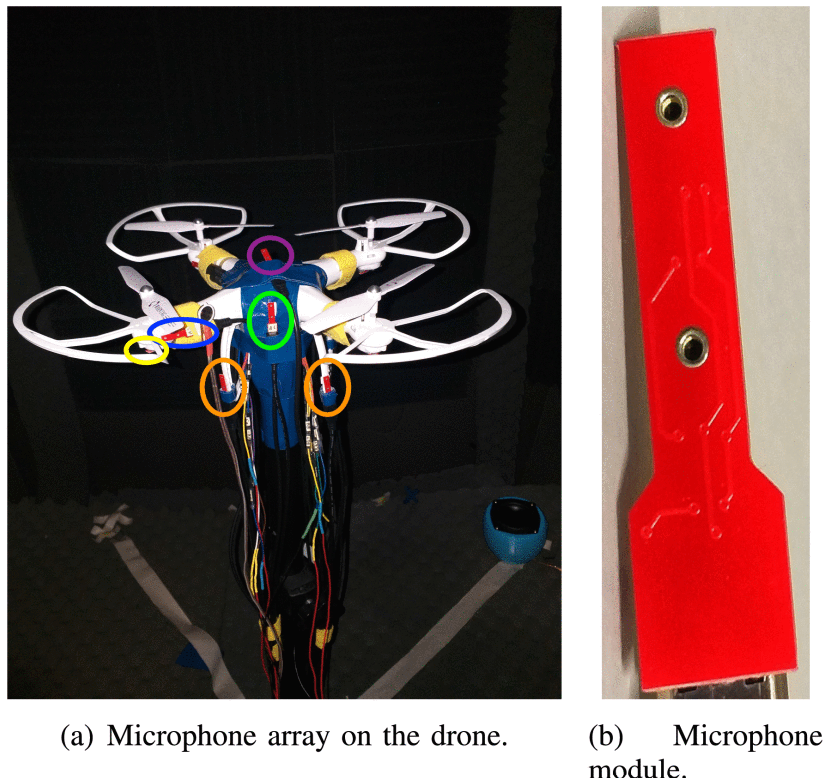
\includegraphics[width=0.75\textwidth]{./manamperi_2022/array.png}
\centering
\caption{The microphone array on the drone (a) and each pair (b) in \cite{manamperi_drone_2022}}
\label{fig:manamperi_2022_array}
\centering
\end{figure}

\begin{figure}[H]
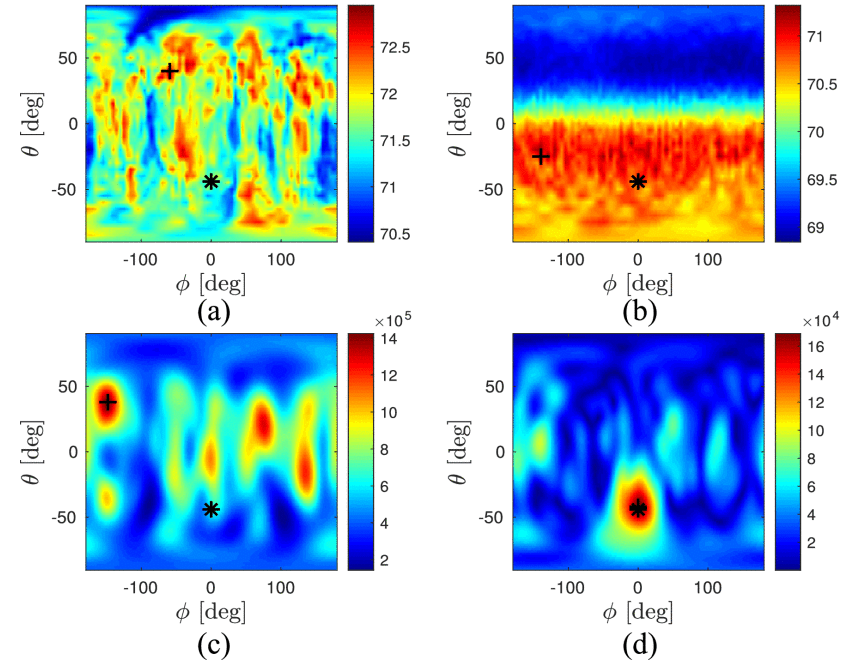
\includegraphics[width=0.75\textwidth]{./manamperi_2022/map_n30.png}
\centering
\caption{The energy maps for MUSIC (a), GEVD-MUSIC (b), GCC-PHAT (c), and the proposed method (d) at an SNR of -30 \si{dB} in \cite{manamperi_drone_2022}}
\label{fig:manamperi_2022_map_n30}
\centering
\end{figure}

\section{Beam-forming}

Beam-forming is a common technique in signal-processing and in many applications for both sound and radio. It is a method of setting many sensors or transmitters in such an array that waves at particular angles and areas constructively interfere to form a beam focused either on a chosen spot or in a chosen direction. Traditionally, it has been used in telecommunications so that multiple radio antennae form a beam that selectively transmits only in one direction. Here, for sound-source-localisation, it is used to steer a beam or a focus in a chosen direction or on a chosen spot so that the energy only from that location is measured. If the beam is steered in enough directions, then an energy map as a function of direction, e.g. azimuth, is made. Another use that may be on interest in this project is that it can be used to spatially filter in a given direction.

One advantage of beamforming over basic localisation through TDOA is that multiple sources can be easily located since the method spatially filters, i.e. it only receives signals from a particular direction or space \cite{rascon_localization_2017}. However, if two sources are near enough to each other, then the resolution of the energy-map may not distinguish the two.

However, there are few considerations \cite{argentieri_survey_2015}:
\begin{itemize}
	\item The more microphones there are, the fewer side lobes or beams there are which show up beside the main lobe or beam.
	\item The further apart the microphones are, the narrower the beam is; this is particularly a problem for robotics where the room on a robot for an array is small.
	\item The beam from the delay-and-sum beamformer is wider at lower frequencies; this affects the resolution and precision for locating sources of lower frequencies.
	\item Copies of the main lobe appear for high frequencies; this is a form of spatial aliasing. A Shannon spatial sampling theorem is given as $d<c/(2f_{\text{max}})$ \cite{argentieri_survey_2015}.
\end{itemize}

\subsection{Delay-and-Sum}

The simplest kind of beamforming is delay-and-sum beamforming where the signal from each microphone is delayed such that the overall sum of all the delayed signals corresponds to a steered direction \cite{rascon_localization_2017}. This sum is maximum when it is steered towards the source. The delay-and-sum beamformer's output steered at the position $\vec{r}_0$ for $M$ microphones is given as the average power:
\begin{equation}
y_{\vec{r}_0}[t] = \sum_{m=1}^M x_m[t-\tau_m(\vec{r}_0)] 
\end{equation}
where $x_n$ is the signal from the $m$-th microphone, and $\tau(\vec{r}_0)$\footnote{One must keep in mind that this is not same as the TDOA estimated from the GCC-PHAT in TDOA-based methods. In fact, this particular method of beamforming highlights the subtle relationship between the two methods, namely TDOA-based and beamforming.} is the time-delay at the $m$-th microphone corresponding at the position $\vec{r}_0$ \cite{argentieri_survey_2015}. In the far field, this output can be simplified to a direction, e.g. $\theta_0$ or $\vec{u}$, instead of a position:
\begin{equation}
y_{\theta_0}[t] = \sum_{m=1}^M x_m[t-\tau_m(\theta_0)] 
\end{equation}
This output can yield an energy-map as:
\begin{equation}
E_{\vec{r}_0} = \sum_{t=1}^T y_{\vec{r}_0}[t]^2
\end{equation}
or
\begin{equation}
E_{\theta_0} = \sum_{t=1}^T y_{\theta_0}[t]^2
\end{equation}

Given a direction $\vec{u}_0$, the expected TDOA can be computed as:
\begin{equation}
\Delta t_{ij} = \tau_{i}(\vec{u}_0) - \tau_{j}(\vec{u}_0) = \frac{f_s}{c} \left( \vec{r}_i - \vec{r}_j \right) \cdot \vec{u}_0
\end{equation}
where $f_s$ is the sampling frequency, $c$ is the speed of sound, $\vec{r}_m$ is the position of the $m$-th microphone. 

A more general kind of beamforming is filter-and-sum beamforming where the signal from each microphone is filtered by its own linear filter rather than delayed \cite{argentieri_survey_2015}. The beamformer's output is given as:
\begin{equation}
y_{\vec{r}_0}[t] = \sum_{m=1}^M w_m(\vec{r}_0)[t]x_m[t]
\end{equation} 
where $w_m(\vec{r}_0)[t]$ is the impulse-response of the $m$-th linear filter.

\subsection{Steered Response Power}

Indeed, the beamformer energy can be computed in a different way using the cross-correlations of many microphones \cite{valin_localization_2004} \cite{valin_robust_2007} \cite{argentieri_survey_2015} \cite{rascon_localization_2017}. This has often been called the steered response power (SRP) and allows faster computation and spectral weighting \cite{badali_evaluating_2009}. 

As said before, the delay-and-sum beamformer is written as:
\begin{equation}
y_{\vec{u}_0}[t] = \sum_{m=1}^M x_m[t-\tau_m(\vec{u}_0)] 
\end{equation}
where $x_m$ is the signal from the $m$-th microphone, and $\tau_m(\theta)$ is the time-delay at the $m$-the microphone from the source given a direction $\vec{u}$ in the far field. This output can yield an energy-map as:
\begin{equation}
E_{\vec{u}} = \sum_{t=1}^T y_{\vec{u}_0}[t]^2
\end{equation}
given a frame $T$ samples long. This can be rewritten in terms of cross-correlations:
\begin{equation}
\begin{split}
E_{\vec{u}} &= \sum_{t=1}^T \left( \sum_{m=1}^M x_m[t-\tau_m(\vec{u}_0)] \right)^2 \\
&= \sum_{m=1}^{M} \sum_{t=1}^T x_m[t - \tau_m(\vec{u}_0)]^2 \\
&+ 2 \sum_{m_1=1}^M \sum_{m_2=1}^{m_1-1} 
\sum_{t=1}^T x_{m_1}\left(t - \tau_{m_1}(\vec{u}_0)\right) x_{m_2}\left(t - \tau_{m_2}(\vec{u}_0)\right) \\
E_{\vec{u}} &= K 
+ 2 \sum_{m_1=1}^M \sum_{m_2=1}^{m_1-1} R_{m_1,m_2} (\tau_{m_1}(\vec{u}_0) - \tau_{m_2}(\vec{u}_0))
\end{split}
\end{equation}
where $R_{ij}$ is the cross-correlation between the $i$-th and the $j$-th microphone, and $K = \sum_{m=1}^{M} \sum_{t=1}^T x_m[t - \tau_m(\vec{u}_0)]^2$ is nearly constant \cite{valin_localization_2004} \cite{valin_robust_2007}. 

Therefore, the beamformer's energy can be simply computed as the sum of cross-correlations for all pairs of microphones. Since the cross-correlation can be computed in the frequency-domain as talked about before in Section-\ref{Time_Difference_of_Arrival}, then a spectral weighting can be used, and other techniques used in estimating the TDOA such as GCC-PHAT can also be used. In fact, SRP with PHAT is known as SRP-PHAT.

\subsection{Literature Examples}

\subsubsection{Valin et al., 2004, Localization of Simultaneous Moving Sound Sources for Mobile Robot Using a Frequency- Domain Steered Beamformer Approach}

A robotic implementation \cite{valin_localization_2004} was done where the beamformer's energy was calculated as the SRP in the frequency-domain using the cross-correlation weighted similarly to the authors' work with estimating the TDOA \cite{valin_robust_2003}. The authors claim that the spectral whitening before computing the beamformer's energy helps narrow the peaks. Here, the authors also proposed a spherical search-grid of 2562 points seen in Figure-\ref{fig:valin_2007_grid} where the beamformer's energy of each is computed. This grid yields a resolution of about 2.5 \si{\degree}. The direction, i.e. both the azimuth and the elevation, of the loudest source is found when the beamformer's energy is maximum. Thereafter, the cross-correlation is zeroed for that loudest source, and the search is repeated for the next loudest source. This is done for a predicted number of sources. If there are fewer sources than the set number, then a source is falsely detected. To handle this, the authors employed probabilistic post-processing to temporally smooth the estimations. Furthermore, in their experiments, they applied two estimators working together, namely a short-term estimator for two sources and a medium-term one for four. 

The experiments were performed with with eight microphones in an open rectangular prism ($0.5\times 0.4\times 0.36$ \si{m}) on top of a mobile robot in "a noisy environment with moderate reverberation"; in fact, this is the same array and robot in the authors' former work \cite{valin_robust_2003} as seen before in Figure-\ref{fig:valin_2003_robot}. The computation was done on a desktop PC and used about 30\% of the CPU. Firstly, the detection-rate was tested against distance for three kinds of sounds, namely hands clapping, speech, and a burst of white noise 250 \si{ms} long. The system was able to detect these sounds reliably up to 5 \si{m}, but drops around 7 \si{m}. The authors claimed that narrowband signals such as tones and speech were detected worse, whilst those with a broader band, such as noise, could be detected much better at longer distances. Furthermore, the estimated azimuth was accurate for four moving speakers although struggled to detect seven. Similar accuracies for both the azimuth and the elevation were given when the robot was moving instead; the authors claim that this demonstrates the robustness against the noise of the motors. Lastly, the array was shown to still be able work when it was not completely open.

\begin{figure}[H]
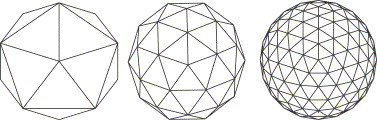
\includegraphics[width=0.75\textwidth]{./valin_2007/grid.jpg}
\centering
\caption{The evolution of the search-grid of 2562 points used in \cite{valin_robust_2003} and in \cite{valin_robust_2007}}
\label{fig:valin_2007_grid}
\centering
\end{figure}

\subsubsection{Valin et al., 2007, Robust Localization and Tracking of Simultaneous Moving Sound Sources Using Beamforming and Particle Filtering}

The same authors later used the same beamforming method but with a particle filter instead \cite{valin_robust_2007}. It also involved a refined search after detecting a source that also estimated distance, but this estimated range was found to be too unreliable. It did however improve the accuracy of the direction in the near field. This new approach was tested on two different arrays on a different mobile robot seen in Figure-\ref{fig:valin_2007_array}. The first array, C1, was an open cube of eight microphones 15.5 \si{cm} wide, whilst the second, C2, was a closed square of four about 40 \si{cm} wide on the robot's chest. 

The experiments were tested in two different environments; the first environment, E1, was a medium-sized room with a reverberation time of 350 \si{ms} at - 60 \si{dB}, whilst the second, E2, was a hall with a reverberation-time of 1.0 \si{s}. In the first environment E1, the open array C1 detected sources more reliably than the closed array C2 within seven metres; C2 struggled to detect hand-claps specifically. Again, in E1, the RMS error for both the azimuth and the elevation was at worst 1.10 \si{\degree} for C1 and at worst 1.44 \si{\degree}. As before, experiments where either multiple sources were moving or the robot was moving were tested in both E1 and E2 as well as where the trajectories of two sources intersect. In such results, the system was deemed to track successfully as seen in Figure-\ref{fig:valin_2007_track}. 

Unlike the one before, this paper also discusses the computation needed, namely for the cross-correlation. For 1024 samples at 48 \si{kHz}, eight microphones, and 2562 searched directions, the complexity is claimed to be only 48.4 \si{Mflops} after counting all time-frequency transformations.

\begin{figure}[H]
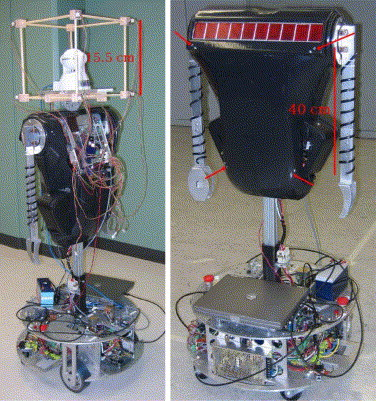
\includegraphics[width=0.75\textwidth]{./valin_2007/array.jpg}
\centering
\caption{The two different microphone arrays on the mobile robot, namely C1 on the left and C2 on the right, tested in \cite{valin_robust_2007}}
\label{fig:valin_2007_array}
\centering
\end{figure}

\begin{figure}[H]
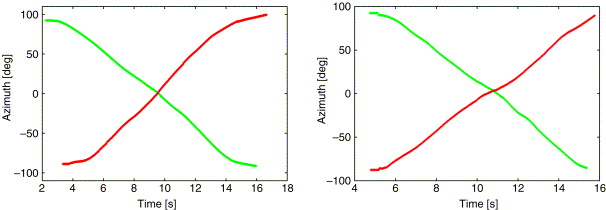
\includegraphics[width=0.75\textwidth]{./valin_2007/track.jpg}
\centering
\caption{The estimated azimuth of two tracked sources crossing paths tested in E1 on the left and in E2 on the right in \cite{valin_robust_2007}}
\label{fig:valin_2007_track}
\centering
\end{figure}

\subsubsection{Badali et al., 2009, Evaluating Real-Time Audio Localization Algorithms for Artificial Audition in Robotics}

A further study \cite{badali_evaluating_2009} compared different variations and strategies of this kind of beamforming as well as the classic estimation of TDOA through GCC-PHAT. Here, TDOA-estimation from the peak of the GCC-PHAT (PEAK) was compared against a classic beamformer, called the steered-response-power (SRP) by the authors. Two variations were also considered, namely spectral weighting (SW) against SNR as proposed in \cite{valin_robust_2003}, \cite{valin_localization_2004}, \cite{valin_robust_2007} and direction-refinement (DR) as also studied in \cite{valin_robust_2007}. The latter is where a local search with a finer resolution is done after the initial search. Furthermore, two search grids are compared, namely a spherical rectangular grid (R) tessellated at 3600 points and a triangular element grid (T) of 2562 points. A cubical array of eight microphones with dimensions of 32 by 32 by 36 \si{cm} seen in Figure-\ref{fig:badali_2009_array} was tested. 

The experiments were done in a room with a reverberation-time of 0.1 \si{s}. The source playing pre-recorded sequences of speech was set at five points of different angle and distance as well as at two heights, one level with the robot and the other at the height of a human. The SNR received was varied by lowering the volume of the source. Two distinct experiments were done; in the first, only the background noise affected the accuracy which was observed to be Gaussian; in the second, a source of classical music as noise was set at only one of the tested positions. In the experiments, the mean error was measured against the SNR, and anomalies where the error was more than 10 \si{\deg} were counted as a percentage. From the results in Figure-\ref{fig:badali_2009_error_SNR}, the triangular grid was deemed better than the rectangular one given that the latter's resolution was not uniform and more concentrated at the poles of the sphere. Overall, the SRP with the SW performed worse than that without. The authors explained that this might have been the difficulty in estimating the noise spectrum. Furthermore, the SRP with the SW had more anomalies. The SRP was found to be better than the classic PEAK estimator.

\begin{figure}[H]
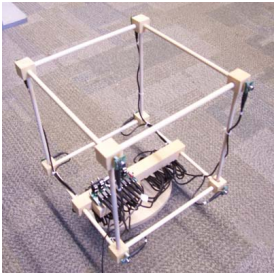
\includegraphics[width=0.75\textwidth]{./badali_2009/array.png}
\centering
\caption{The microphone array tested in \cite{badali_evaluating_2009}}
\label{fig:badali_2009_array}
\centering
\end{figure}

\begin{figure}[H]
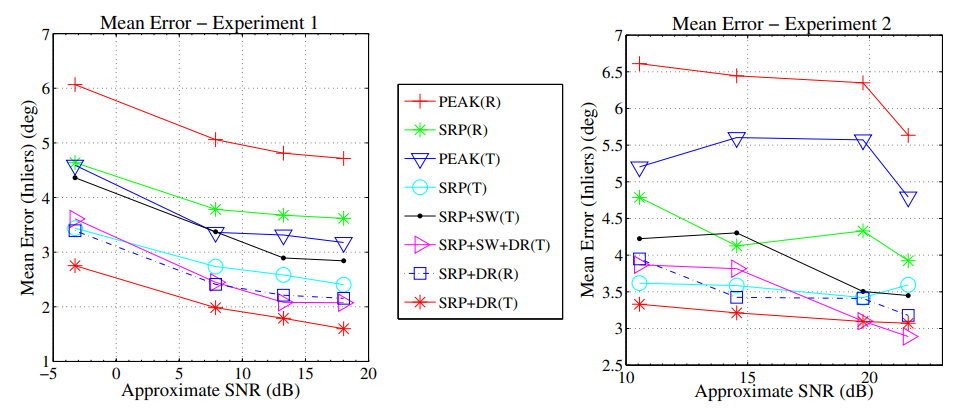
\includegraphics[width=0.75\textwidth]{./badali_2009/error_SNR.png}
\centering
\caption{The mean angular error as a function of SNR for different methods and configurations in \cite{badali_evaluating_2009}}
\label{fig:badali_2009_error_SNR}
\centering
\end{figure}

\subsubsection{Salvati et al., 2019, Power Method for Robust Diagonal Unloading Localization Beamforming}

A more recent paper \cite{salvati_power_2019} proposed diagonal unloading on a beamformer so that the system could work with high noise. This diagonal unloading was done by subtracting a diagonal matrix from the covariance matrix of the array's signal. In the robust design, the covariance matrix was estimated by the largest eigenvalue of the array's signal which was computed by the power method. This robust design was evaluated in simulation and compared against the suboptimal design using diagonal unloading, SRP-PHAT, and MUSIC. 

The array was a uniform circle of eight microphones with a radius of 20 \si{cm}, and the spatial resolution was 5 \si{\degree}. As seen in Figure-\ref{fig:salvati_2019_RMSE_SNR}, when there was a single source, the RMS error in angle of the proposed design was at most about 2.5 \si{\degree} for an SNR of at least -10 \si{dB} and grew for worse SNR. As seen in Figure-\ref{fig:salvati_2019_RMSE_SNR_two}, when there were two sources, the RMS error was at most about 4 \si{\degree} for an SNR of at least -5 \si{dB}. In all cases, the proposed robust design worked better than SRP-PHAT and suboptimal design and did just as well as MUSIC. Furthermore, despite working just as well as MUSIC, the authors claimed that their proposed design has much simpler computation of $O(M^2)$ instead of that of $O(M^3)$ where $M$ is the number of microphones.

\begin{figure}[H]
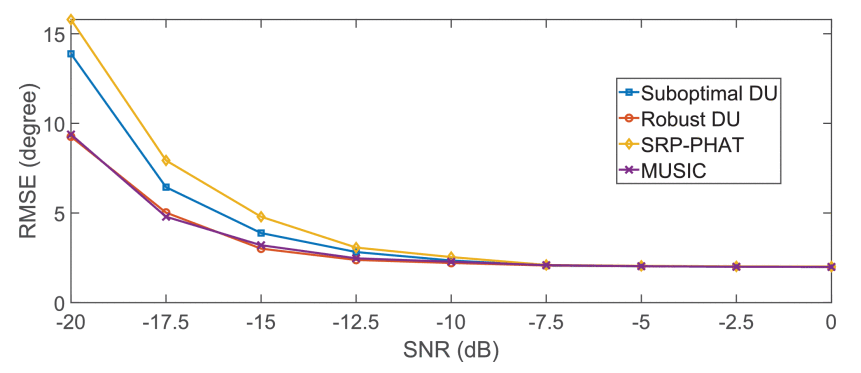
\includegraphics[width=0.75\textwidth]{./salvati_2019/RMSE_SNR.png}
\centering
\caption{The RMS error as a function of SNR for a single source in \cite{salvati_power_2019}}
\label{fig:salvati_2019_RMSE_SNR}
\centering
\end{figure}

\begin{figure}[H]
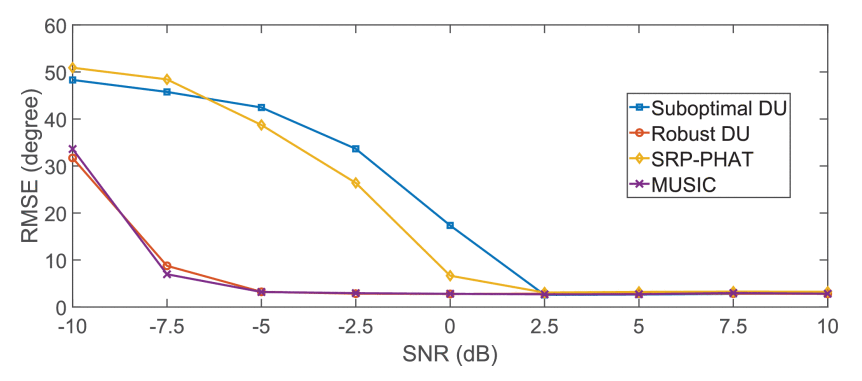
\includegraphics[width=0.75\textwidth]{./salvati_2019/RMSE_SNR_two.png}
\centering
\caption{The RMS error as a function of SNR for two sources in \cite{salvati_power_2019}}
\label{fig:salvati_2019_RMSE_SNR_two}
\centering
\end{figure}

\subsubsection{Basiri et al., 2016, On-Board Relative Bearing Estimation for Teams of Drones Using Sound}

Robotics is not the only application for localisation by beamforming. Autonomous drones are often imagined with the same capabilities of sound-source-localisation. One such study \cite{basiri_-board_2016} proposed SRP-PHAT but with a modified PHAT weighting with a power factor to mitigate the effect of noise. In order to localise multiple neighbouring drones, it also proposed a system inspired by \cite{brutti_multiple_2010} of pruning the next dominant source in the computed cross-correlation. The paper evaluated both a passive method of localising other drones' engine-sounds and an active method of localising other drones' beacons. 

The passive method which is the most relevant was tested indoors with a resting drone localising a flying drone. Motion-tracking was used to measure the true positions. The authors disclaimed that the sound of cooling fans belonging to eight tracking cameras and two computers could be heard in the room. For a single flying drone, the angular RMS error was 1.39 \si{\degree} as seen in Figure-\ref{fig:basiri_2016_histogram}. For multiple flying drones, the resting drone could localise at most three, and the precision worsen dramatically for the fourth. The array used for the passive method was a flat T-shape of four microphones seen in Figure-\ref{fig:basiri_2016_array}. The authors did not say what the exact dimension were. This study is of particular interest to robotics given that the system seemed to have been implemented on an embedded system on a drone, but the authors did not discuss computation, etc.

\begin{figure}[H]
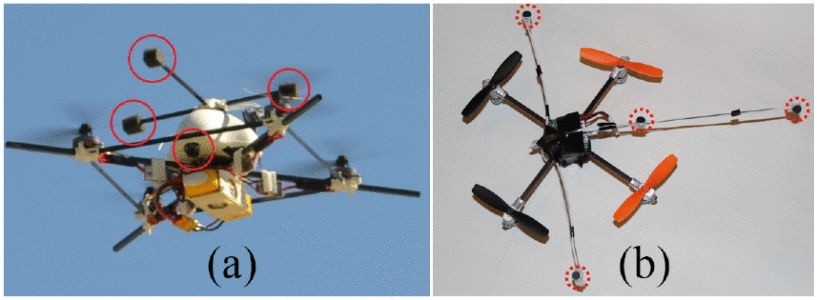
\includegraphics[width=0.75\textwidth]{./basiri_2016/array.png}
\centering
\caption{The two different microphone arrays tested in \cite{basiri_-board_2016}, namely one for the active method (a) and another for the passive method (b),}
\label{fig:basiri_2016_array}
\centering
\end{figure}

\begin{figure}[H]
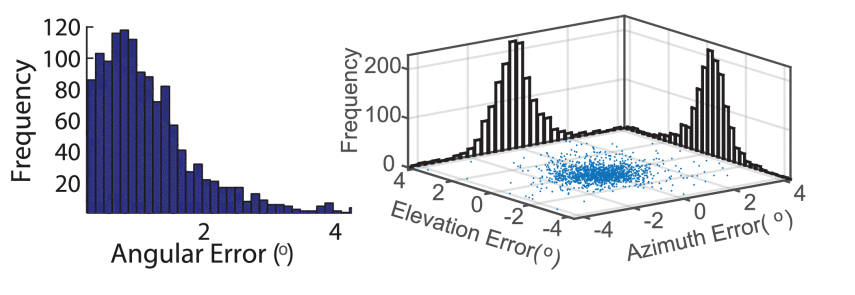
\includegraphics[width=0.75\textwidth]{./basiri_2016/histogram.png}
\centering
\caption{The histogram of the angular error for the passive method in \cite{basiri_-board_2016}}
\label{fig:basiri_2016_histogram}
\centering
\end{figure}

\section{MUSIC}

One branch of methods used to analyse and locate sound-sources separates the space of signals into subspaces. The most common kind of which is multiple-signal-classification (MUSIC). This method has a very high resolution but generally has a high computational burden, especially compared to that of TDOA or beamforming. Therefore, it is not explored as in depth as before, but the general performance across the literature is given.

The basic idea behind MUSIC is that the signals received by an array of microphones is split into subspaces, each representing either a signal or a noise. The model for the signal received is:
\begin{equation}
X = W_s S + V
\end{equation}
where 
\begin{itemize}
	\item each row of $X\in \mathbb{C}^{M\times F}$ is the received signal of the $m$-th microphone $x_m$ in the frequency-domain, i.e. $X_m$,
	\item each row of $S\in \mathbb{C}^{N\times F}$ is the $n$-th source's signal $s_n$ in the frequency-domain, i.e. $S_n$,
	\item each row of $V\in \mathbb{C}^{M\times F}$ is the noise of the $m$-th microphones in the frequency-domain,
	\item $W_s\in \mathbb{C}^{M\times S}$ is a weighting that models the time-delays of each source at each microphone for a given direction or position,
\end{itemize}
and where $M$ is the number of microphones, $F$ is the number of samples, frequency-points, etc., and $N$ is the number of sources, i.e. signals \cite{rascon_localization_2017}.

Given this, the overall goal of MUSIC is to split the space of signals into two subspaces, namely one for signals and another for noise. This is done by eigen-decomposition of the sampled covariance matrix $R[f]\in \mathbb{C}^{N\times N}$ for a given frequency $f$.

The most basic form of MUSIC, known as standard eigen-value-decomposition (SEVD), finds the eigen-decomposition of the covariance matrix as the following:
\begin{equation}
R[f] = Q[f]\Lambda[f]Q^{-1}[f]
\end{equation}
where $\Lambda[f]$ is a diagonal matrix of the $M$ eigenvalues $\lambda_m[f]$, and each column of $Q[f]$ is a corresponding eigenvector $q_m[f]$. This matrix of eigenvectors is often split into two subspaces, $Q[f] = [Q_s[f]|Q_n[f]]$, the former for signals, and the latter for noise \cite{rascon_localization_2017}. Thereby, the spatial spectrum is found from the orthogonality between the steered direction and the eigenvectors for noise:
\begin{equation}
P(\theta_0, \phi_0)[f] = \frac{\lvert A^*(\theta_0, \phi_0) A(\theta_0, \phi_0) \rvert}
	{\sum_{m=\tilde{N}+1}^M \lvert A^*(\theta_0, \phi_0) q_m[f] \rvert}
\end{equation}
where $\tilde{N}$ is the number of sources considered, and $A(\theta_0, \phi_0)\in \mathbb{C}^{M\times 1}$ is the steering vector of transfer-functions at each microphone for a given three-dimensional direction\footnote{Much like beamforming, a full three-dimensional position can more generally be considered rather than only a direction, but again like before, this only works reliably in the near field. Since the far field is much more relevant to a small array on a robot, only direction has been considered in this example.}, i.e. an azimuth $\theta_0$ and an elevation $\phi_0$ \cite{nakamura_real-time_2012}. More simply, each row is often the lag $e^{-2\pi f\tau_m}$ where $\tau_m$ is the time-delay at the $m$-th microphone corresponding to the given direction \cite{rascon_localization_2017}.

This spatial spectrum however is narrowband for one point or bin of frequency. For a broadband response, the narrowband response is averaged over the given band of frequencies \cite{ishi_effects_2011} \cite{nakamura_real-time_2012}.

An extension of SEVD is general eigen-value-decomposition (GEVD) where the noise is whitened before the decomposition \cite{nakamura_intelligent_2009} \cite{nakamura_intelligent_2011} \cite{nakamura_real-time_2012}. Here, the eigen-decomposition is such:
\begin{equation}
K^{-1}[f] R[f] = Q[f] \Lambda[f] Q^{-1}[f]
\end{equation}
where $K[f]$ is a freely chosen matrix but is often computed as $N[f]N^*[f]$ where $N[f]$ is the frequency-domain noise recorded when there are no signals. This is shown to be more robust than SEVD for a SNR less than 0 \si{dB}.

\subsection{Literature Examples}

\subsubsection{Ishi et al., 2009, Evaluation of a MUSIC-Based Real-Time Sound Localization of Multiple Sound Sources in Real Noisy Environments}

One paper \cite{ishi_evaluation_2009} proposed a form of broadband SEVD-MUSIC where the output was the average of all the narrowband responses over a frequency-range. This was done for a small array of fourteen microphones around a robot's neck and chest as seen in Figure-\ref{fig:ishi_2009_array}. This proposed system estimated both the azimuth and the elevation on a discrete spherical grid with a resolution of about 5 \si{\degree}. Since MUSIC needs a known number of sources, the authors proposed a fixed number of sources for the narrowband MUSIC response and a maximum number of sources from the broadband response. They also compare the magnitude against a threshold to find whether the peak was a source or not. Multiple sources were nevertheless found by sequentially subtracting a two-dimensional Gaussian centred where the next highest source was; this approach is similar to others \cite{brutti_multiple_2010}, \cite{basiri_-board_2016}. 

The paper evaluated this system for a range of parameters, namely number of FFT points, frequency-range, and value of the threshold. The system was tested in a variety of "noisy environments", namely an office where the main sources of noise were an air-conditioner and the robot's hardware and an outdoor shopping mall, but the authors did not tell under what SNR and reverberation the system was tested. Nevertheless, the authors found that the system could run in real time given 64 FFT points for each frame which was about 4 \si{ms} long. Furthermore, the authors found that a frequency-range from 1 to 6 \si{kHz}, a threshold of 1.7, a fixed number of sources of 2, and a maximum number of sources of 5 were best. In most of the experiments, the accuracy was around 80 \% successful detection-rate.

\begin{figure}[H]
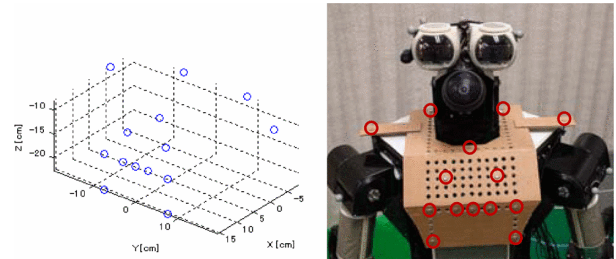
\includegraphics[width=0.75\textwidth]{./ishi_2009/array.png}
\centering
\caption{The microphone array on the robot tested in \cite{ishi_evaluation_2009}}
\label{fig:ishi_2009_array}
\centering
\end{figure}

\subsubsection{Nakamura et al., 2012, Real-Time Super-Resolution Sound Source Localization for Robots}

Another kind of MUSIC is called GEVD-MUSIC which is more robust to noise, especially the noise more powerful than the wanted signal itself. An early paper \cite{nakamura_intelligent_2009} that first proposed this kind of MUSIC in the context of robotics compared the accuracy of GEVD-MUSIC as a percentage to that of SEVD-MUSIC. The accuracy of the latter dropped below an SNR of around 5 \si{dB} whilst the accuracy of GEVD-MUSIC kept at 100 \% at an SNR of around -7 \si{dB}. In a later paper \cite{nakamura_intelligent_2011}, many of the same authors proposed the same method but with a audio-visual integration with a particle filter for tracking inactive sources and hierarchical Gaussian mixture-models. Again, the accuracy of SEVD-MUSIC dropped at an SNR of around -8 \si{dB}, whilst that of GEVD-MUSIC dropped at an SNR of around -14 \si{dB}. 

To ease the computation, the same authors proposed a new kind of MUSIC called GSVD-MUSIC \cite{nakamura_real-time_2012}. To further lessen computation, the authors proposed a hierarchical search from coarse to fine, and to improve the resolution, they linearly interpolated the transfer-functions in both the frequency- and time-domain. The accuracy of the proposed GSVD-MUSIC only began to drop at an SNR fo around -10 \si{dB}, about 5 \si{dB} less than that of GEVD-MUSIC. The average error in the azimuth was at best about 1 \si{\degree} and at worst about 10 \si{\degree}. The proposed method also worked well for a moving source. The array was a circle of eight microphones embedded in the robot's head. The authors claimed that their new method of GSVD-MUSIC lessened the computational cost by 40.6 \% compared to GEVD-MUSIC and that their design of a hierarchical search lessened it by a further 59.2 \% for a single source. However, the computation was done on a laptop, and no comparison was made with other methods of sound-source-localisation such as SRP-PHAT.
% discussion: array on head

\begin{figure}[H]
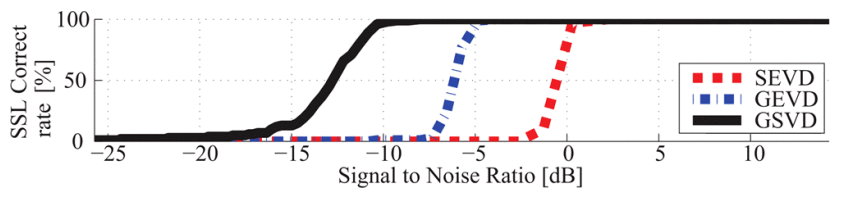
\includegraphics[width=0.75\textwidth]{./nakamura_2012/rate_SNR.png}
\centering
\caption{The rate of successful localisations against SNR for SEVD, GEVD, and the proposed GSVD in \cite{nakamura_real-time_2012}}
\label{fig:nakamura_2012_rate_SNR}
\centering
\end{figure}

\section{Discussion of the Literature}

Many examples and methods in the literature have been discussed. Here, a summary of the most relevant findings.

Nearly all methods only compute the three-dimensional angle. Only one attempted full three-dimensional position, i.e. direction along with distance \cite{chen_sound_2019}. seemed to attempt this in the far field for distances more than 1 \si{m}; one pap for example \cite{bechler_system_2004} only tested within about 1 \si{m} which may considered to be the near field given the dimensions of their array. Most methods tended to have an error of 2 \si{\degree}.

As for noise, Manamperi et al. in 2022 \cite{manamperi_drone_2022} tested up to the worst SNR of -30 \si{dB} although this paper was specifically about mitigating noise in the context of drones.

Most methods could run in real-time albeit on laptop and desktop computers. However, Basiri et al. in 2016 \cite{basiri_-board_2016} seemed to be the only example implemented on an embedded system on the drone itself, namely an Atmel AVR32 microcontroller. This example is therefore of particular interest to this project given the want for an embedded implementation.


\chapter{Preliminary Simulations} \label{Preliminary_Simulations}

Before the technique and the algorithm are chosen, some of the techniques talked about in the literature-review must first be evaluated and further studied. Here, this chapter looks at two techniques or methods, an iterative algorithm and a steered-response beamformer. The code for the simulations is too tedious to include in this report; thus, it is available in this project's GitHub repository\footnote{Note that there may be commits afterwards.}: \url{https://github.com/Claegtun/fyp-nubots-ssl}.

\section{Software}

This section lists the specific software and resources that were used to simulate.

\subsection{Python}

Most of the simulations have been done in Python which is a free and popular programming language that has many free and open-source third-party libraries to help simulate physical and mathematical phenomena. It also has many tools to help plot data and concepts.

Some Python modules used are:
\begin{itemize}
	\item numpy which has many mathematical functions,
	\item scipy which has some signal-processing functions,
	\item matplotlib which is a plotting tool,
	\item and pyroomacoustics.
\end{itemize}

\subsection{Pyroomacoustics}

One very important aspect of the simulation was to emulate the effect of a room on the sound recorded by a microphone. This is commonly taken as the reverberation or more specifically the reverberation-impulse-response (RIR) which can be used to compute the sound recorded by convolution on the original.

A very helpful Python module was that called Pyroomacoustics which was made specifically for simulating arrays of microphones. It could compute the RIR given the dimensions of a room, the location of the source, the location of the microphone, and other parameters such as the absorption-factor of the walls. The module mainly uses the image-source model (ISM) which is a common model for reverberation as well as optionally ray-tracing. It could also simulate with an array of microphones and superpose noise on the signal.

It also had a suite of functions and examples for sound-source-localisation, but these were mostly ignored since the purpose of the simulations was to recreate existing examples in the literature and to study the methods from first principles.

\subsection{Sounds}

For sounds, a variety of sounds were taken from \textit{freesound.org} which has a corpus of free and public recordings of sounds mostly under the Attribution 4.0 licence \footnote{https://creativecommons.org/licenses/by/4.0/}.

\section{Evaluation of Examples in the Literature}

In order to choose the best method for this project, some of the examples in the literature must first be evaluated in the simulation, especially against the effects of noise and reverberation. So far in this project, only two examples were studied, namely:
\begin{itemize}
	\item the TDOA-based and iteration-based method used on a rectangular pyramid array that can estimate the distance as well as the direction \cite{chen_sound_2019}
	\item and the common SRP-PHAT method used for beamforming \cite{valin_localization_2004} \cite{valin_robust_2007}.
\end{itemize}

%\subsection{Analysis of GCC-PHAT}

\subsection{Rectangular Pyramid Array with TDOA}

One example in the literature that stands out is the paper describing an array as a rectangular pyramid on a mobile robot \cite{chen_sound_2019} since it is one of the few examples that claim to estimate distance as well as direction. The estimation of distance is a highly valuable ability in this project. Therefore, it was the first example to evaluate.

\subsubsection{Algorithm}

As said before, the array was a rectangular pyramid 0.25 \si{m} wide and 0.125 \si{m} tall as seen in Figure-\ref{fig:chen_2019_array}. The algorithm described in the paper \cite{chen_sound_2019} was seemingly complex. It worked on one frame of signals, i.e. a block of samples representing a duration of time. Each frame was made up of multiple channels for each microphone, in this case, five channels. 

Firstly, the TDOA was estimated for each pair, or permutation, of microphones. The matrix of which was averaged diagonally in magnitude only since there was some redundancy in mirrored TDOAs, i.e. $\Delta t_{ij} = -\Delta t_{ji}$. Since the algorithm used an iterative approach, it needed an initial guess. The paper described albeit vaguely a strategy of comparing TDOAs of adjacent pairs. This would break the space up into eight sectors or partitions in one of which the source lied. Given a lack of detail in the paper, this was interpreted as in Algorithm-\ref{alg:pyramid_guess}.

\begin{algorithm}[H]
\caption{Guessing the general direction from a rectangular pyramid}
\label{alg:pyramid_guess}
\begin{algorithmic}
	\For{every $i$-th microphone on the corners of the pyramid's base}
		\State $a \gets$ the index of the left adjacent microphone
		\State $b \gets$ the index of the right adjacent microphone
		\For{$j = a, b$}
			\State Get the TDOA as $\Delta t_{ji}$
		\EndFor
		\If{$\Delta t_{ai} > 0$ \textbf{ and } $\Delta t_{bi} > 0$}
			\If{$\Delta t_{ai} > \Delta t_{bi}$}
				\State $k \gets a$
			\Else
				\State $k \gets b$
			\EndIf
			\State $r_i$ is the position of the $i$-th microphone.
			\State $r_k$ is the position of the $k$-th microphone.
			\Comment{The source lies between the sector spanned by the $i$-th microphone and the $k$-th microphone.}
			\State $r \gets 2 (r_{i} + r_{k})$ \Comment{Make a vector that lies within this sector.}
		\EndIf
	\EndFor
\end{algorithmic}
\end{algorithm}

Next, the paper laid out a strategy of calculating four estimates given that only three TDOAs were needed for the iterative algorithm. Here, the top microphone has an index of 0, whilst the others have indices of 1, 2, 3, and 4. Thus, given three TDOAs $\Delta t_{0j}$, the position of the source could be found by the following model:
\begin{equation}
\begin{split}
f_j(x,y,z) &= \sqrt{\left(x-x_j\right)^2 + (y - y_j)^2 + (z - z_j)^2} \\
&- \sqrt{\left(x-x_0\right)^2 + (y - y_0)^2 + (z - z_0)^2}
- c \Delta t_{j0}
\end{split}
\end{equation}
where $j = 1, 2, 3, 4$, and $c$ is the speed of sound.

This was solved by the iterative formula based on Newton's well known method.
\begin{equation}
\begin{bmatrix}
	x^{(k+1)} \\
	y^{(k+1)} \\
	z^{(k+1)}
\end{bmatrix}
=
\begin{bmatrix}
	x^{(k)} \\
	y^{(k)} \\
	z^{(k)}
\end{bmatrix}
-
J^{-1}
\begin{bmatrix}
	f_1\left(x^{(k)}, y^{(k)}, z^{(k)}\right) \\
	f_2\left(x^{(k)}, y^{(k)}, z^{(k)}\right) \\
	f_3\left(x^{(k)}, y^{(k)}, z^{(k)}\right)
\end{bmatrix}
\end{equation}
where $J$ is the Jacobian as such:
\begin{equation}
J = 
\begin{bmatrix}
\frac{\partial f_1}{\partial x}
& \frac{\partial f_1}{\partial y}
& \frac{\partial f_1}{\partial z} \\
\frac{\partial f_2}{\partial x}
& \frac{\partial f_2}{\partial y}
& \frac{\partial f_2}{\partial z} \\
\frac{\partial f_3}{\partial x}
& \frac{\partial f_3}{\partial y}
& \frac{\partial f_3}{\partial z}
\end{bmatrix}
\end{equation}

The paper did not give a maximum number of iterations, but in this study, at most a hundred were tried since the algorithm seemed to find the solution within twenty iterations. Sometimes however, depending on the initial condition, the algorithm would diverge rapidly which would eventually lead to a singular matrix. In the Python simulation, a condition was checked whether the estimated position was further than 100 \si{m} from the array; in which case, it could be safely assumed that the iterative algorithm had failed which was then aborted. This would be counted and logged as a failure.

Since the iterative algorithm only needed three TDOAs from three pairs of the top microphone with the three corner microphones, four estimates could be gotten. These were then averaged to give the final estimated position of the source.

\subsubsection{Experimental Method}

The microphone-array was set 1 \si{m} off the floor in the centre of a closed room 10 \si{m} wide, 10 \si{m} long, and 3 \si{m} high. The rectangular base of the array was also oriented to be in line with the room. Given that the origin was in one bottom corner of the room, the coordinates of the centre of the array's rectangular base were $(5,5,1)$. Furthermore, an absorption factor of 0.5 was used for the walls. This gave RIRs as seen in Figure-\ref{fig:pyramid_robot_noise_rir} and an estimated reverberation-time at 60 \si{dB} of 84.8 \si{ms}. This would roughly emulate a large indoor office-space with moderate reverberation.

\begin{figure}[H]
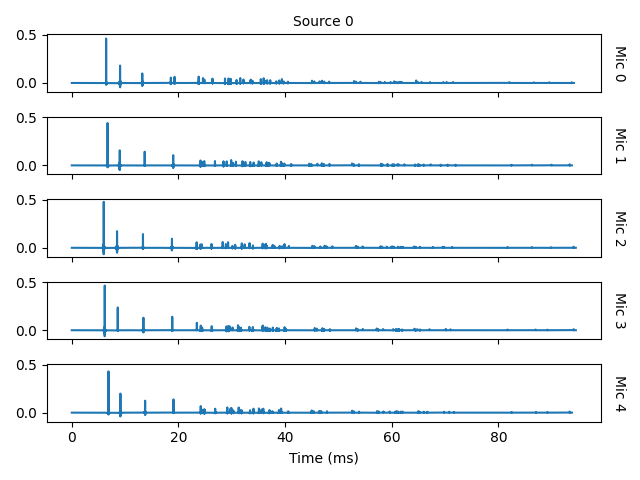
\includegraphics[width=0.9\textwidth]{../Python/pyramid_robot/noise/rir.png}
\centering
\caption{An example of the RIR made from the Pyroomacoustics module is shown.}
\label{fig:pyramid_robot_noise_rir}
\centering
\end{figure}

For the sound, a recording of claps taken in an anechoic chamber was used \cite{noauthor_handclaps_2005}. After it was simulated in the room-environment, a single frame of 8192 samples was analysed in the algorithm.

\subsubsection{Performance against Noise}

The first experiment was to evaluate the performance against noise, specifically additive Gaussian white noise (AGWN). Overall, ten levels of noise were simulated for which, i.e. SNRs from -20 to 25 \si{dB}. For each level of noise, ten thousand runs of the simulation were done in order to calculate the mean and variance of the estimated values. Thereby, the accuracy of the method was given by how much the mean deviates from the true value, and the precision and repeatability were given by how much the variance increases.

The source was fixed with the coordinates of $(5.5,3,1)$ as seen in Figure-\ref{fig:pyramid_robot_room_3d} and -\ref{fig:pyramid_robot_room_2d}. This makes the source 2.06 \si{m} away from the centre of the array with an azimuth of 76.0 \si{\degree} and with an elevation of 90 \si{\degree}.

\begin{figure}[H]
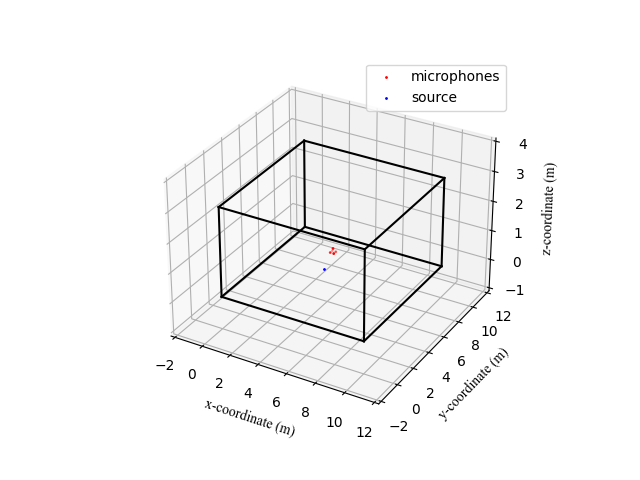
\includegraphics[width=0.9\textwidth]{../Python/pyramid_robot/room_3d.png}
\centering
\caption{The 3D room is shown and has the rectangular pyramid array in the centre 1 \si{m} off the ground and with the source at $(5.5,3,1)$.}
\label{fig:pyramid_robot_room_3d}
\centering
\end{figure}

\begin{figure}[H]
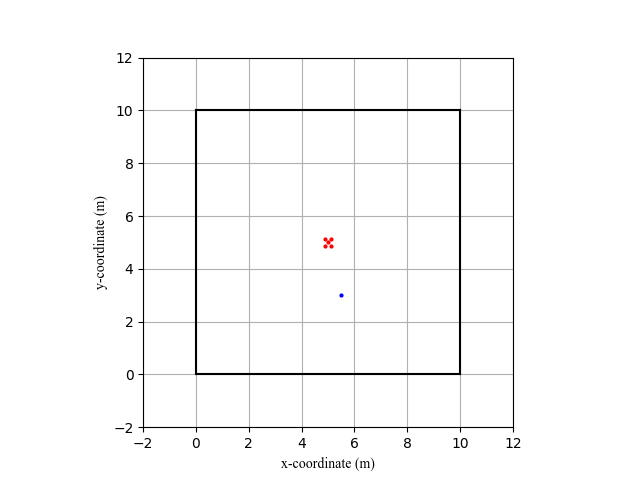
\includegraphics[width=0.9\textwidth]{../Python/pyramid_robot/room_2d.png}
\centering
\caption{A bird's-eye-view of the room is shown with the rectangular pyramid array in the centre 1 \si{m} off the ground and with the source at $(5.5,3,1)$.}
\label{fig:pyramid_robot_room_2d}
\centering
\end{figure}

The performances for the estimated distance, the estimated azimuth, and the estimated elevation are given in Figure-\ref{fig:pyramid_robot_noise_distance}, -\ref{fig:pyramid_robot_noise_azimuth}, and -\ref{fig:pyramid_robot_noise_elevation} respectively.

% Fix the y-axis labels.

\begin{figure}[H]
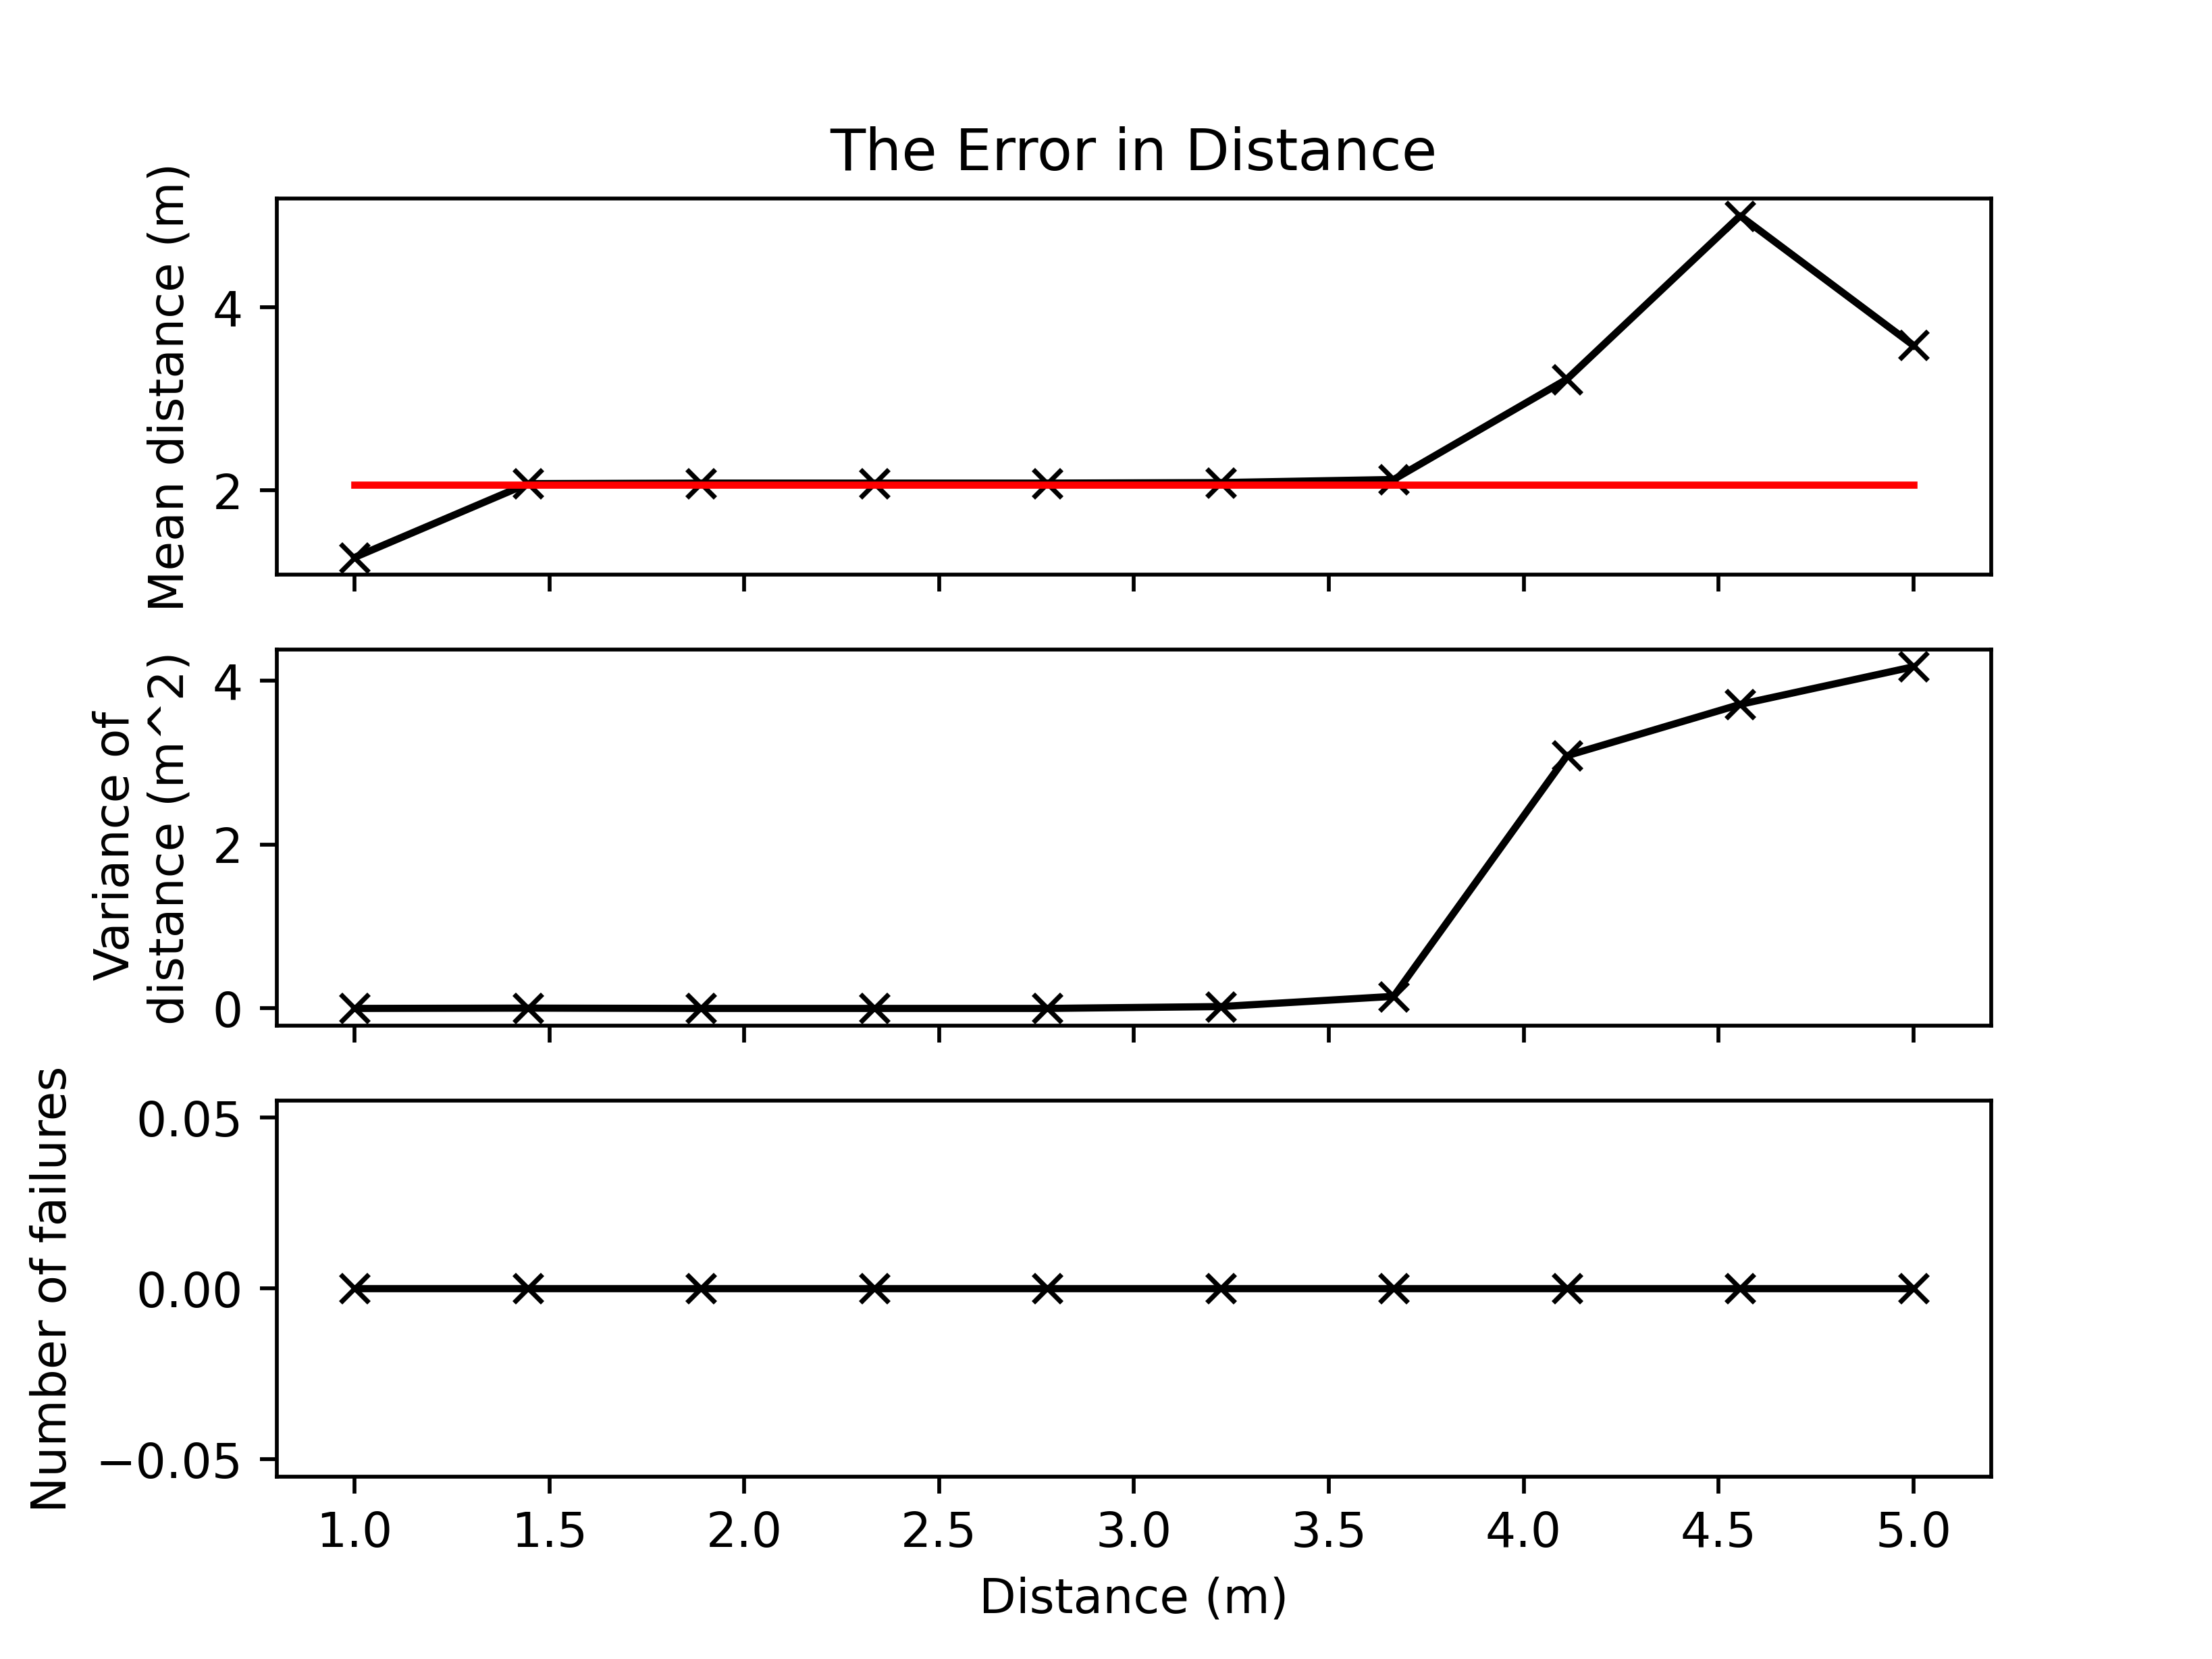
\includegraphics[width=0.9\textwidth]{../Python/pyramid_robot/noise/distance.png}
\centering
\caption{The statistical performance of estimated distance is plotted against noise; the red line is the true distance.}
\label{fig:pyramid_robot_noise_distance}
\centering
\end{figure}

\begin{figure}[H]
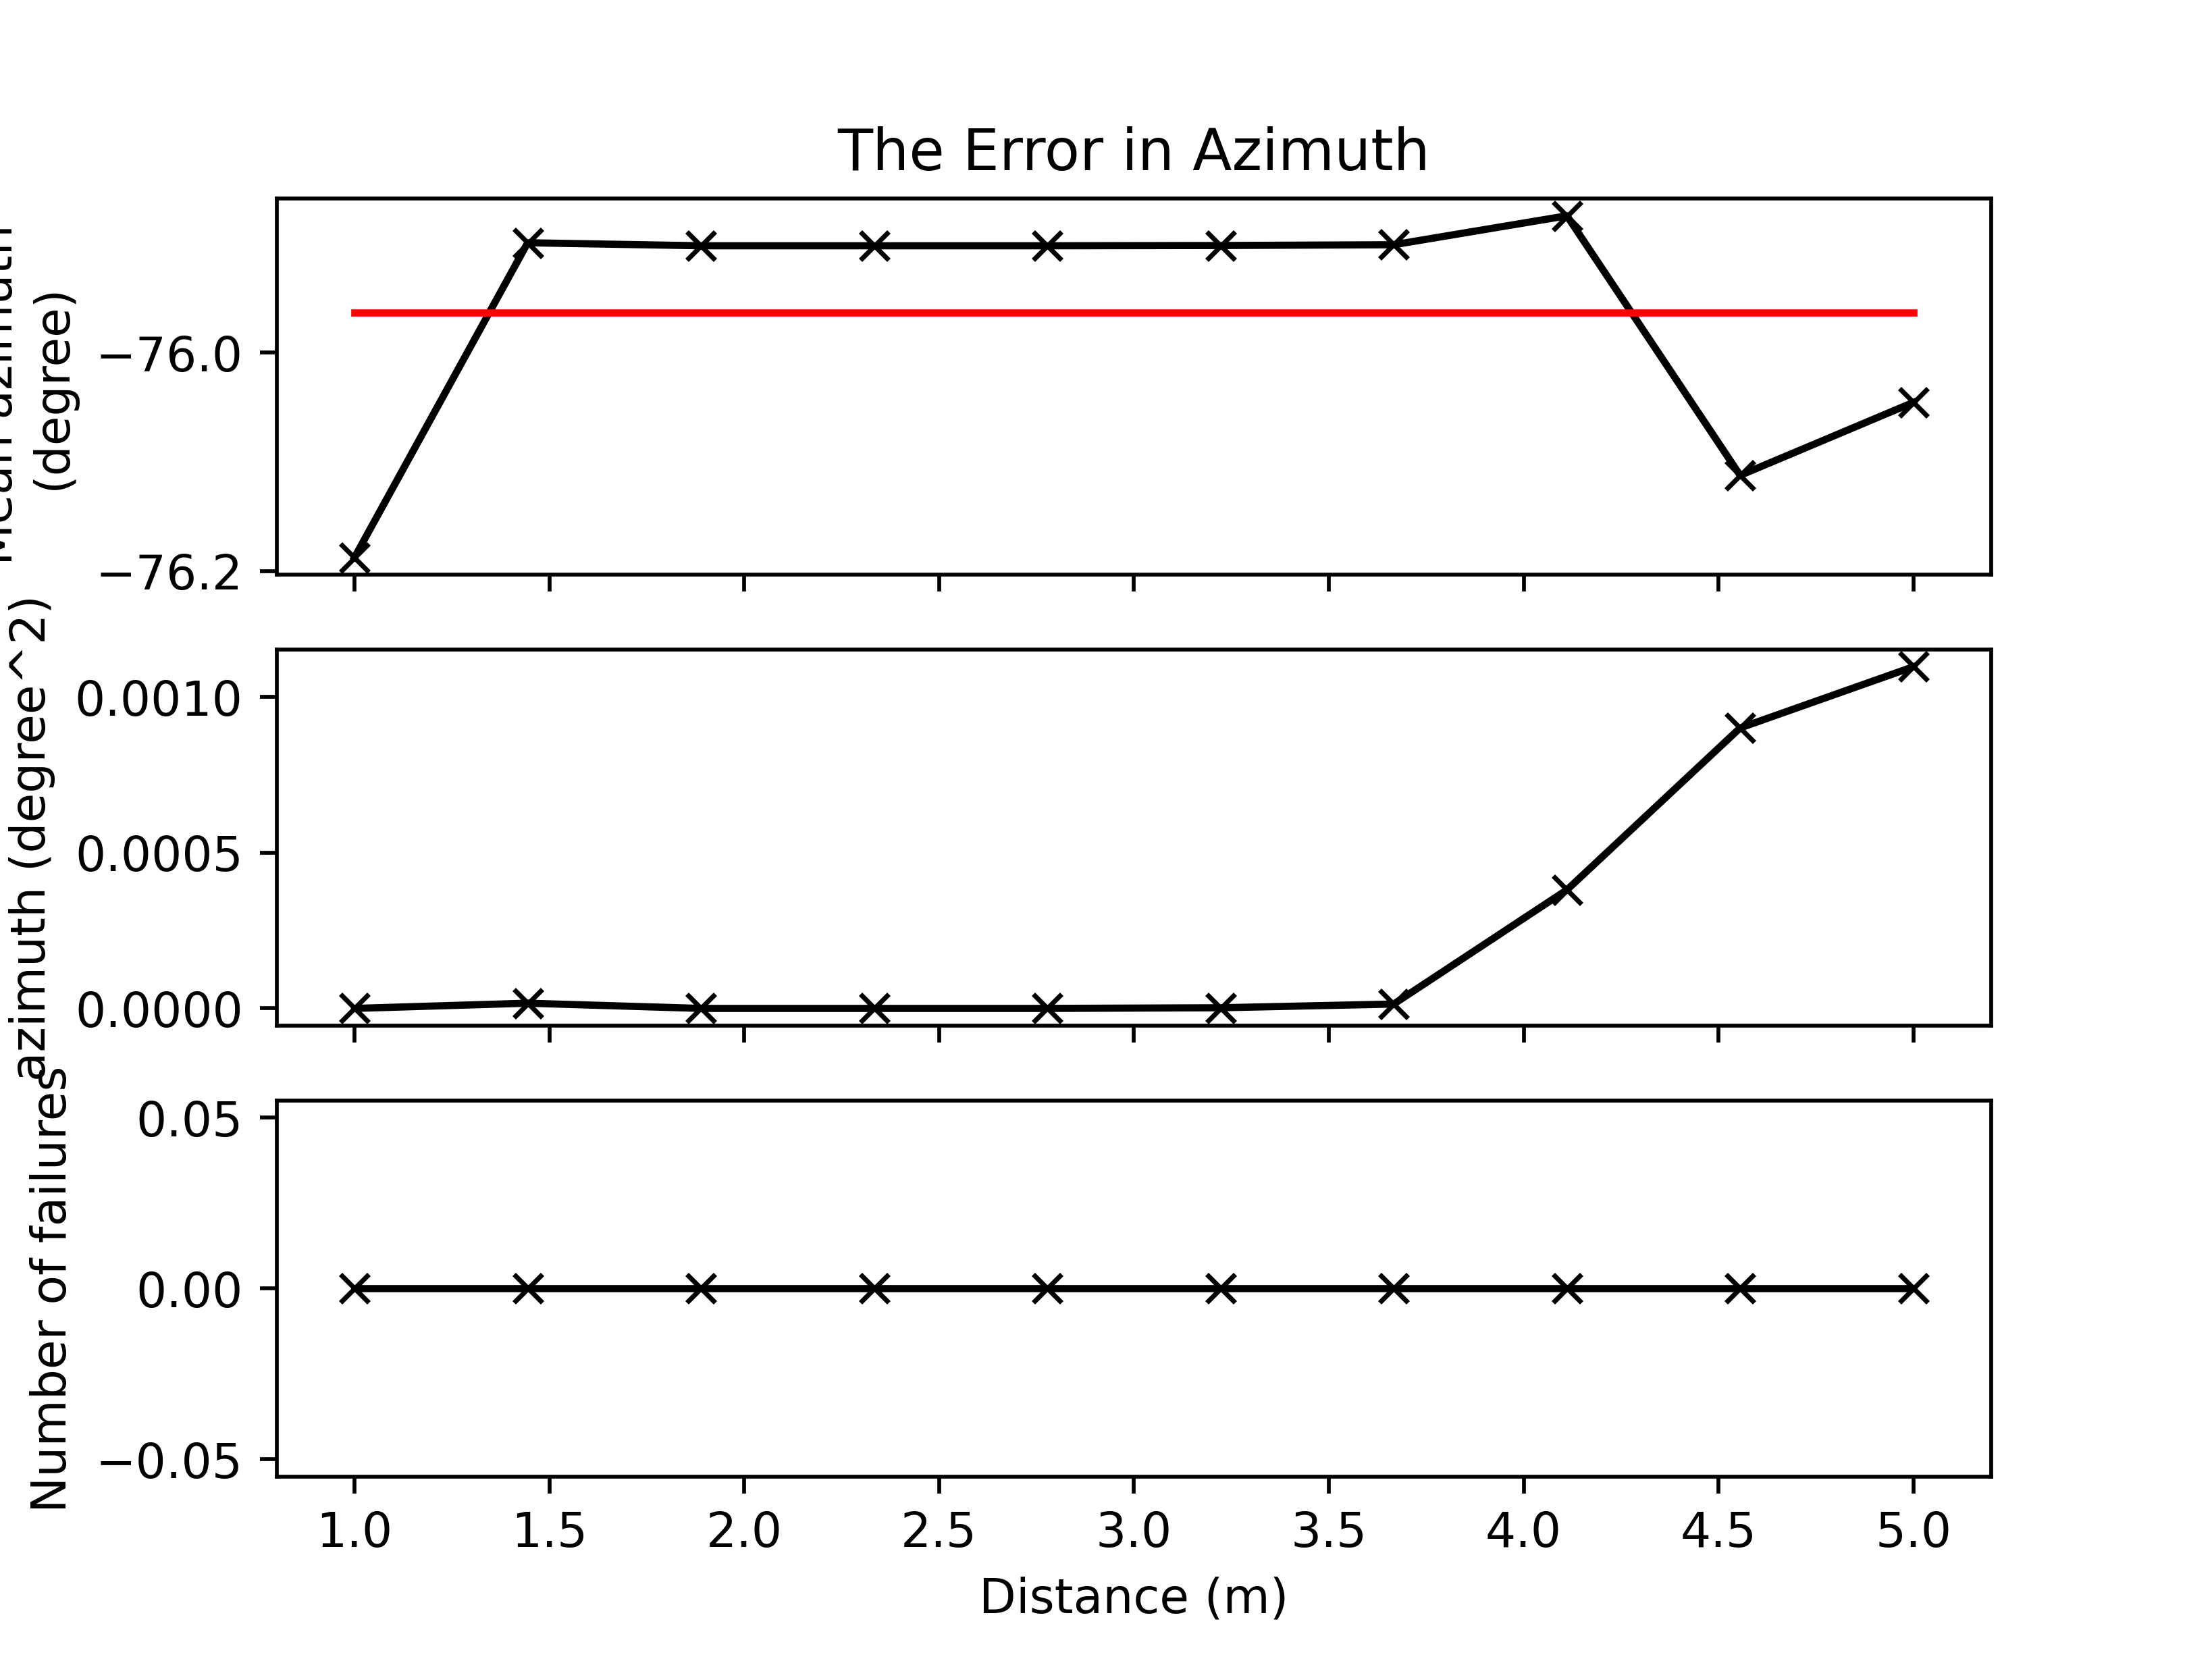
\includegraphics[width=0.9\textwidth]{../Python/pyramid_robot/noise/azimuth.png}
\centering
\caption{The statistical performance of estimated azimuth is plotted against noise; the red line is the true azimuth.}
\label{fig:pyramid_robot_noise_azimuth}
\centering
\end{figure}

\begin{figure}[H]
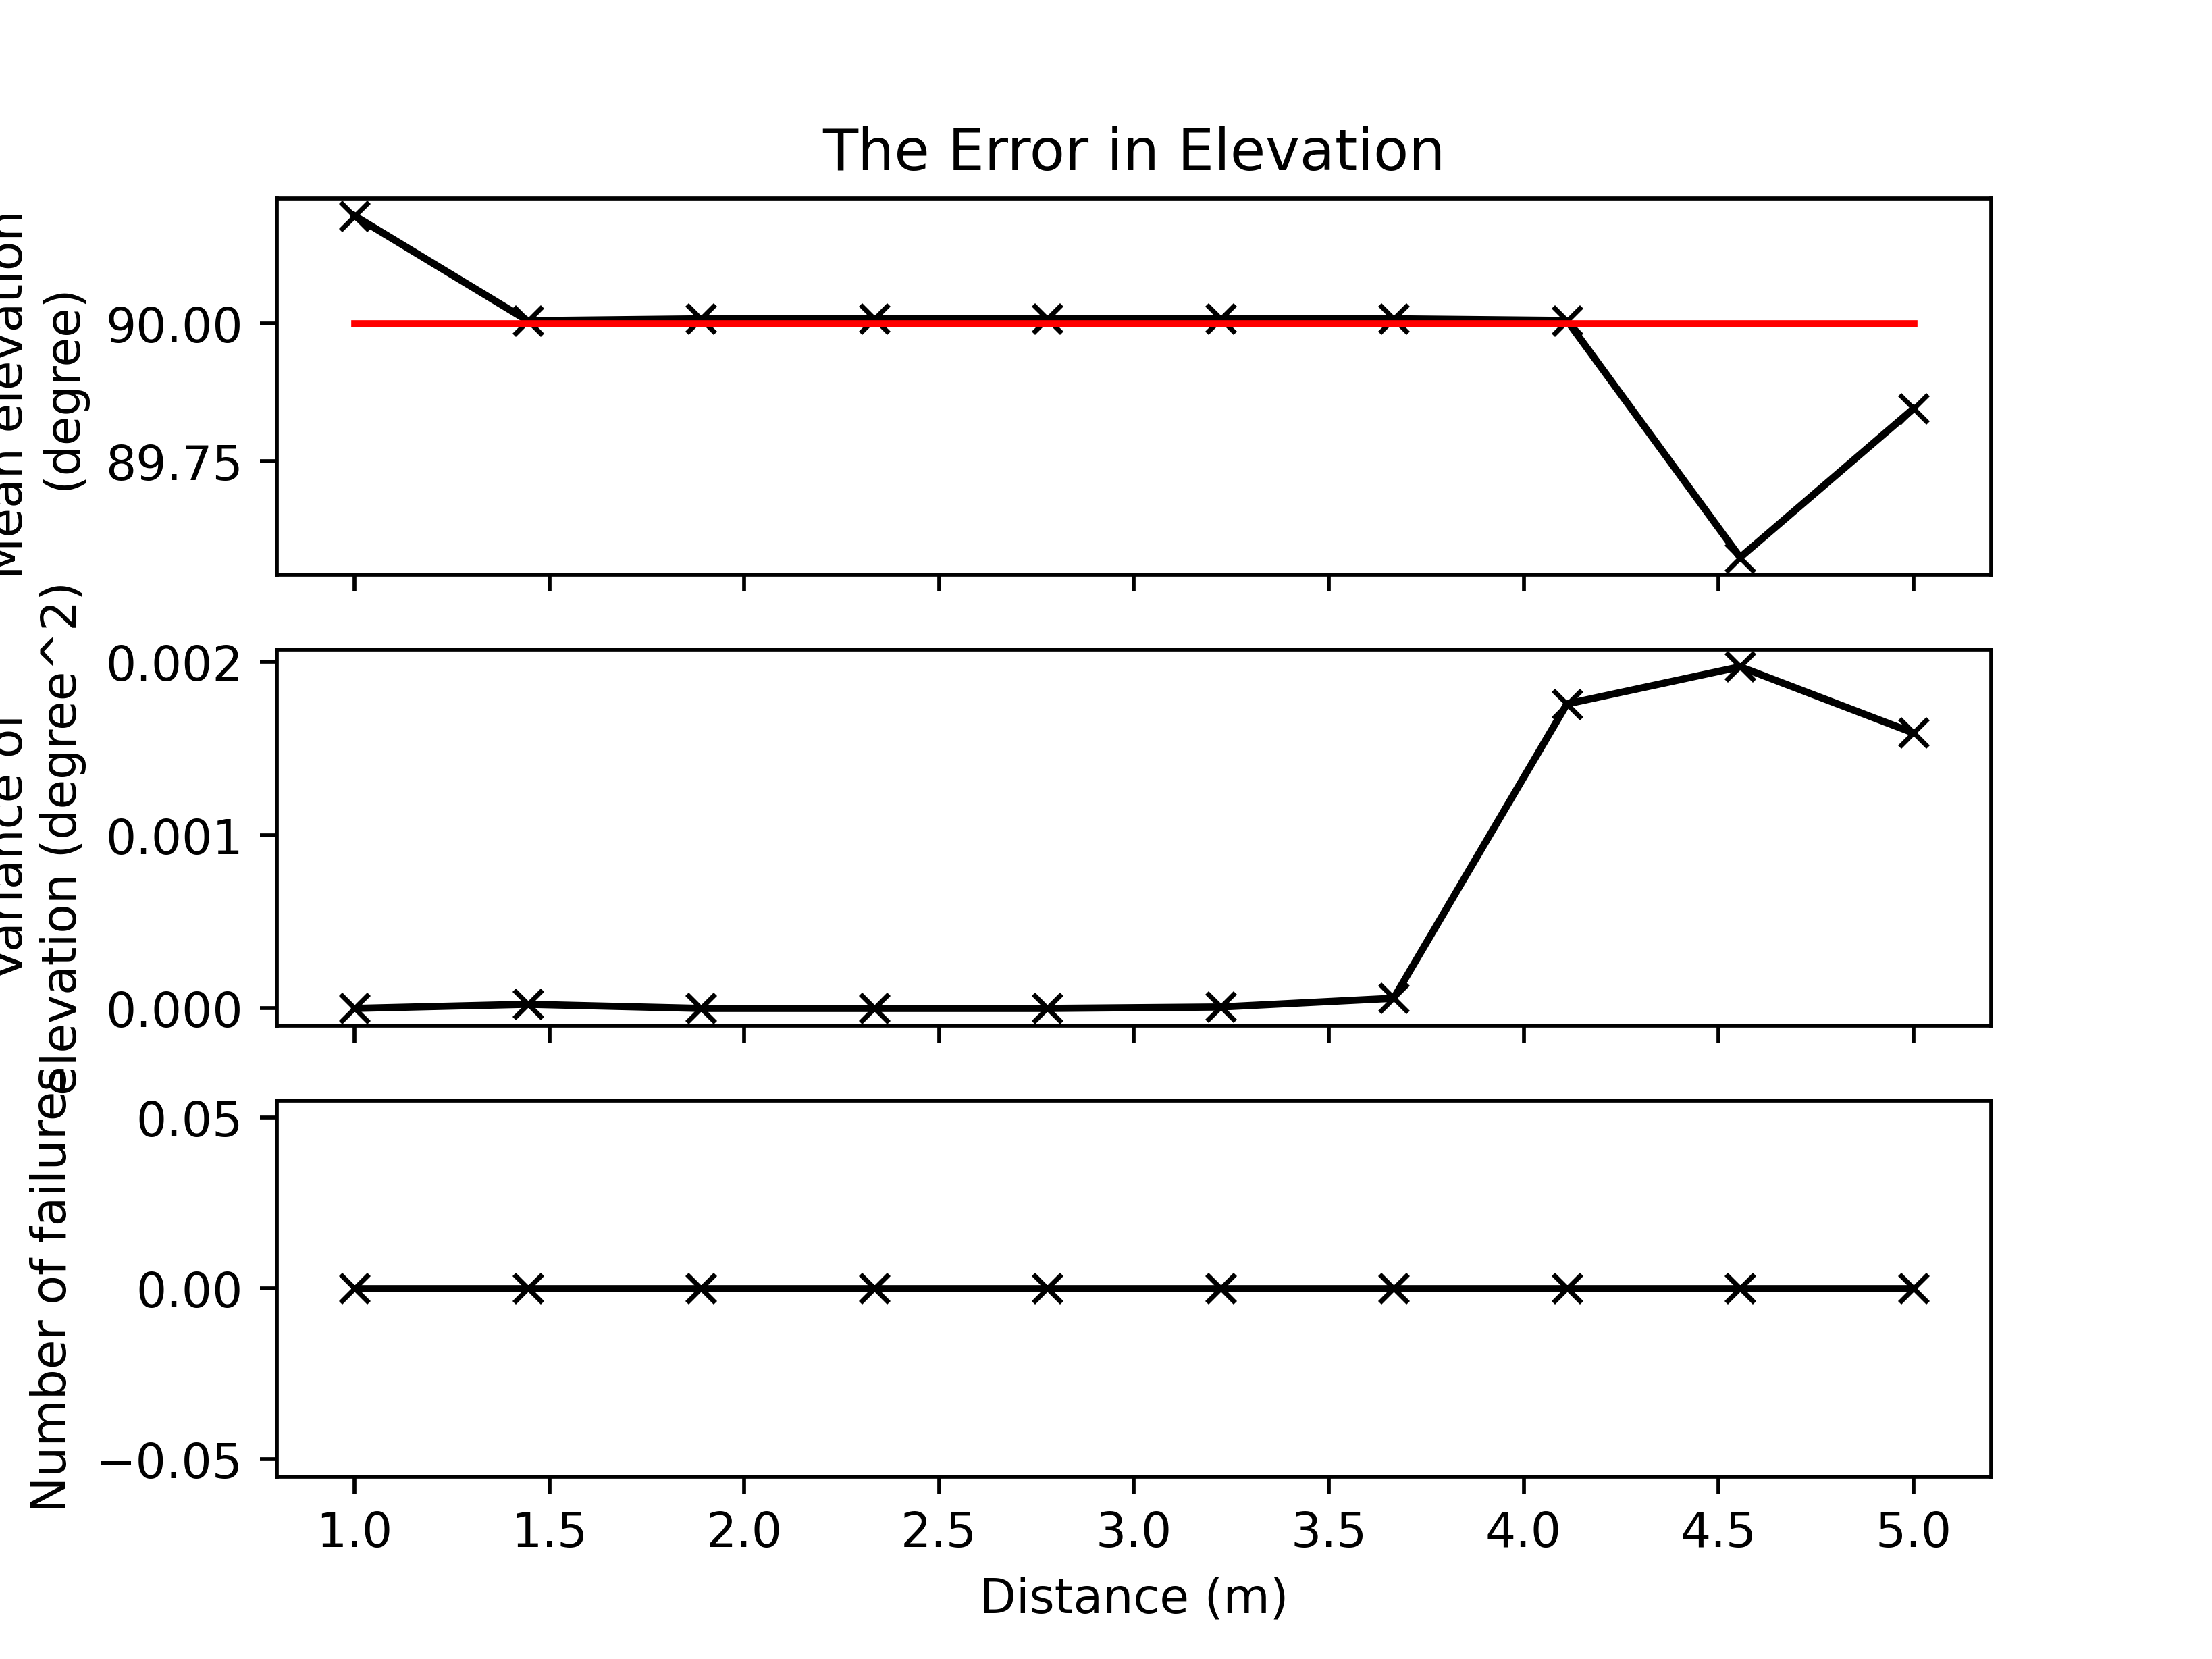
\includegraphics[width=0.9\textwidth]{../Python/pyramid_robot/noise/elevation.png}
\centering
\caption{The statistical performance of estimated elevation is plotted against noise; the red line is the true elevation.}
\label{fig:pyramid_robot_noise_elevation}
\centering
\end{figure}

From these results, the estimated direction, i.e. both the azimuth and the elevation, had very little variance and little bias which albeit became worse with noise. However, the estimated distance was worsened much more as seen in Figure-\ref{fig:pyramid_robot_noise_distance} with high bias and variance. Furthermore, the number of failures in the iterative algorithm became significantly worse as noise was increased. This in fact made the calculation of the mean and the variance for all three values hard since it no longer followed the law of large numbers. This may explain the odd values for the mean and the variance for the first few noise-levels, i.e. towards the left of the plot.

\subsubsection{Performance against Distance}

The next experiment was to evaluate the performance against distance. Overall, ten levels of noise were simulated for which, i.e. SNRs from -20 to 25 \si{dB}. For each level of noise, ten thousand runs of the simulation were done in order to calculate the mean and variance of the estimated values. Thereby, the accuracy of the method was given by how much the mean deviates from the true value, and the precision and repeatability were given by how much the variance increases.

The source was fixed with the coordinates of $(5.5,3,1)$ as seen in Figure-\ref{fig:pyramid_robot_room_3d} and -\ref{fig:pyramid_robot_room_2d}. This makes the source 2.06 \si{m} away from the centre of the array with an azimuth of 76.0 \si{\degree} and with an elevation of 90 \si{\degree}.

\subsubsection{Discussion}

Although it was one of the few that estimates the distance, this method relies on an iterative algorithm and thus relies on an initial condition. It was found in simulation that this iterative algorithm was highly sensitive to inaccurate estimations of the TDOAs. This would often lead to the iterative algorithm failing to converge. This would especially happen if the noise was high which would lead to peaks at zero in the GCC-PHAT and this would give an inaccurate TDOA. This can be clearly seen as the number of failures grew as the noise was increased in Figure-\ref{fig:pyramid_robot_noise_distance}. The iterative algorithm was also found to be sensitive to the choice of the initial condition.

\subsection{SRP-PHAT} \label{SRP_PHAT}

This section will study a common method of beamforming shared among a few papers reviewed so far, namely SRP-PHAT. In particular, it was used on mobile robots \cite{valin_localization_2004}, \cite{valin_robust_2007}.

\subsubsection{Algorithm}

In this simulation, a modified PHAT spectral weighting was used as described in \cite{valin_localization_2004}, and similar to that in \cite{valin_robust_2003}:
\begin{equation}
\psi_{m_i,m_j}(\tau) = \frac{1}{\lvert X_{m_i}(k) \rvert \lvert X_{m_j}(k) \rvert}
\end{equation}
The special weighting is:
\begin{equation}
w(k) =
\begin{cases}
	1,										& Y(k) \leq Y_N(k) \\
	\left( \frac{Y(k)}{Y_N(k)}\right)^\gamma	& Y(k) > Y_N(k)
\end{cases}
\end{equation}
where $\gamma$ is set as 0.1\footnote{This was chosen from \cite{valin_localization_2004} but can be easily tuned if need be.}, $Y(k)$ is the mean spectral density across all microphones, and $Y_N(k)$ is the noise estimate as the average of $Y(k)$ across time. Here, neither paper went into much depth about the calculation of $Y_N(k)$; so, it was assumed that it was the average for all runtime instead of a moving window. This modified weighting would weight frequencies with higher SNR more to lessen the effect of noise and also to better the detection of narrowband signals.

As seen in Figure-\ref{fig:srp_phat_grid}, a spherical grid of 2562 points was used as a search-grid of directions as described in some of the papers \cite{valin_localization_2004} \cite{valin_robust_2007}. This was generated by tessellating an icosahedron.

\begin{figure}[H]
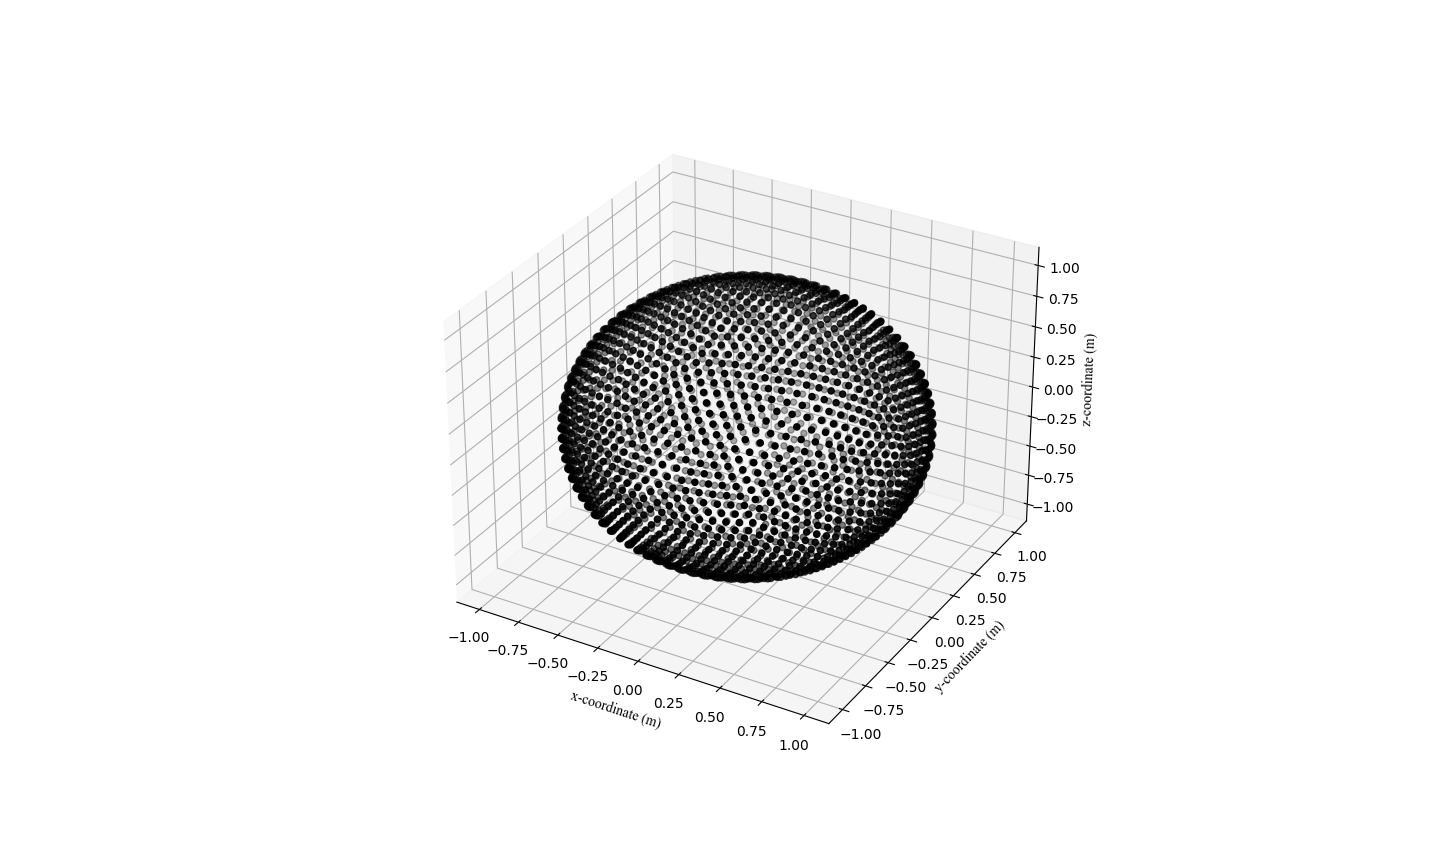
\includegraphics[width=0.9\textwidth]{../Python/srp_phat/grid.png}
\centering
\caption{The spherical grid of directions was used to estimate the direction of the sound-source using SRP-PHAT.}
\label{fig:srp_phat_grid}
\centering
\end{figure}

Each of these points was used as a direction along which to steer the beamformer and thus to draw a spherical energy-map. The direction that corresponded to the highest energy was the estimated direction of the source.

\subsubsection{Experimental Method}

The dimensions of the tested microphone-array were taken from one of the often cited papers for the SRP-PHAT \cite{valin_robust_2007}, namely a cube 15.5 \si{cm} wide. The array was set up the same way as before; that is 1 \si{m} off the floor in the centre of a closed room 10 \si{m} wide, 10 \si{m} long, and 3 \si{m} high. The array was also oriented to be in line with the room. Given that the origin was in one bottom corner of the room, the coordinates of the array's centre were $(5,5,1)$. Furthermore, an absorption factor of 0.5 was used for the walls. This gave RIRs as seen in Figure-\ref{fig:pyramid_robot_noise_rir} and an estimated reverberation-time at 60 \si{dB} of 84.8 \si{ms}. This would roughly emulate a large indoor office-space with moderate reverberation.

For the sound, two kinds were tested; first, a recording of claps taken in an anechoic chamber was used \cite{noauthor_handclaps_2005}; secondly, a recording of a whistle. The former sound models a typical broadband signal, whilst the latter models a typical narrowband signal. These sounds were resampled to 48 \si{kHz} to ensure a consistent analysis.

After it was simulated in the room-environment, a single frame of 1024 samples was analysed in the algorithm, but all other frames before that were analysed to calculate the noise spectral density.

\subsubsection{Stastical Performance against Noise}

The first experiment was to evaluate the performance against noise, specifically additive Gaussian white noise (AGWN). Overall, ten levels of noise were simulated for which, i.e. SNRs from -20 to 25 \si{dB}. Ten thousand runs of the simulation for each noise-level were done in order to calculate the mean and variance of the estimated values. Thereby, the accuracy and the bias of the method was given by how much the mean deviates from the true value, and the precision and repeatability were given by how much the variance increases.

The source was fixed with the coordinates of $(5.5,3,1)$  as seen in Figure-\ref{fig:srp_phat_room_3d} and -\ref{fig:srp_phat_room_2d}. This makes the source 2.06 \si{m} away from the centre of the array with an azimuth of 76.0 \si{\degree} and with an elevation of 90 \si{\degree}.

\begin{figure}[H]
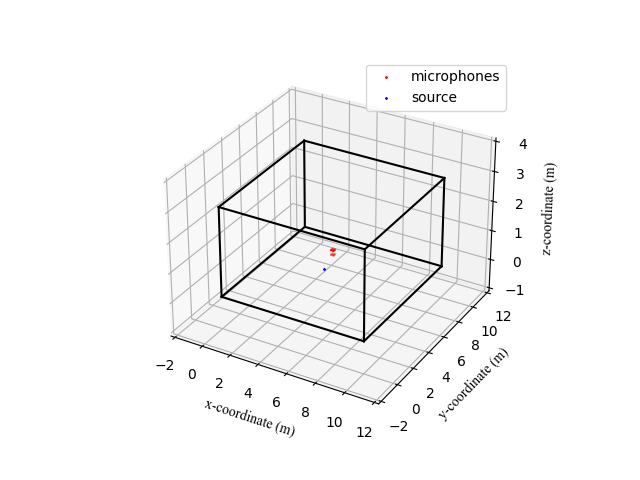
\includegraphics[width=0.9\textwidth]{../Python/srp_phat/room_3d.png}
\centering
\caption{The 3D room is shown and has the cubic array for testing the SRP-PHAT method in the centre 1 \si{m} off the ground and with the source at $(5.5,3,1)$.}
\label{fig:srp_phat_room_3d}
\centering
\end{figure}

\begin{figure}[H]
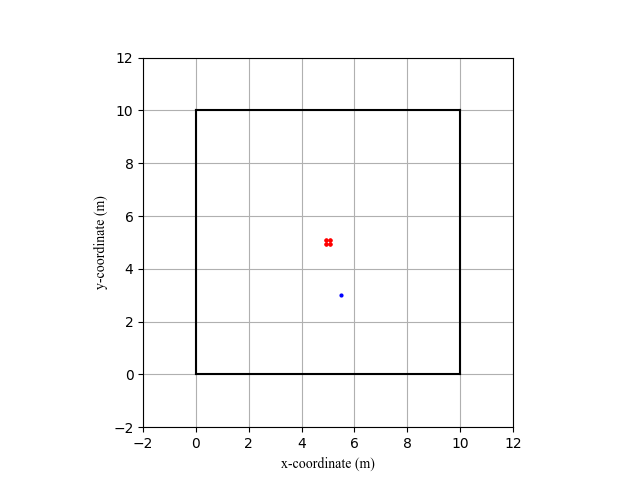
\includegraphics[width=0.9\textwidth]{../Python/srp_phat/room_2d.png}
\centering
\caption{A bird's-eye-view of the room is shown with the cubic array for testing the SRP-PHAT method in the centre 1 \si{m} off the ground and with the source at $(5.5,3,1)$.}
\label{fig:srp_phat_room_2d}
\centering
\end{figure}

The performances for the estimated azimuth and the estimated elevation are given in Figure-\ref{fig:srp_phat_noise_clap} and -\ref{fig:srp_phat_noise_whistle} respectively.

\begin{figure}[H]
\includegraphics[width=0.9\textwidth]{../Python/srp_phat/noise/clap/plots.png}
\centering
\caption{The statistical performance of the estimated direction is plotted against noise with a clap as the source.}
\label{fig:srp_phat_noise_clap}
\centering
\end{figure}

\begin{figure}[H]
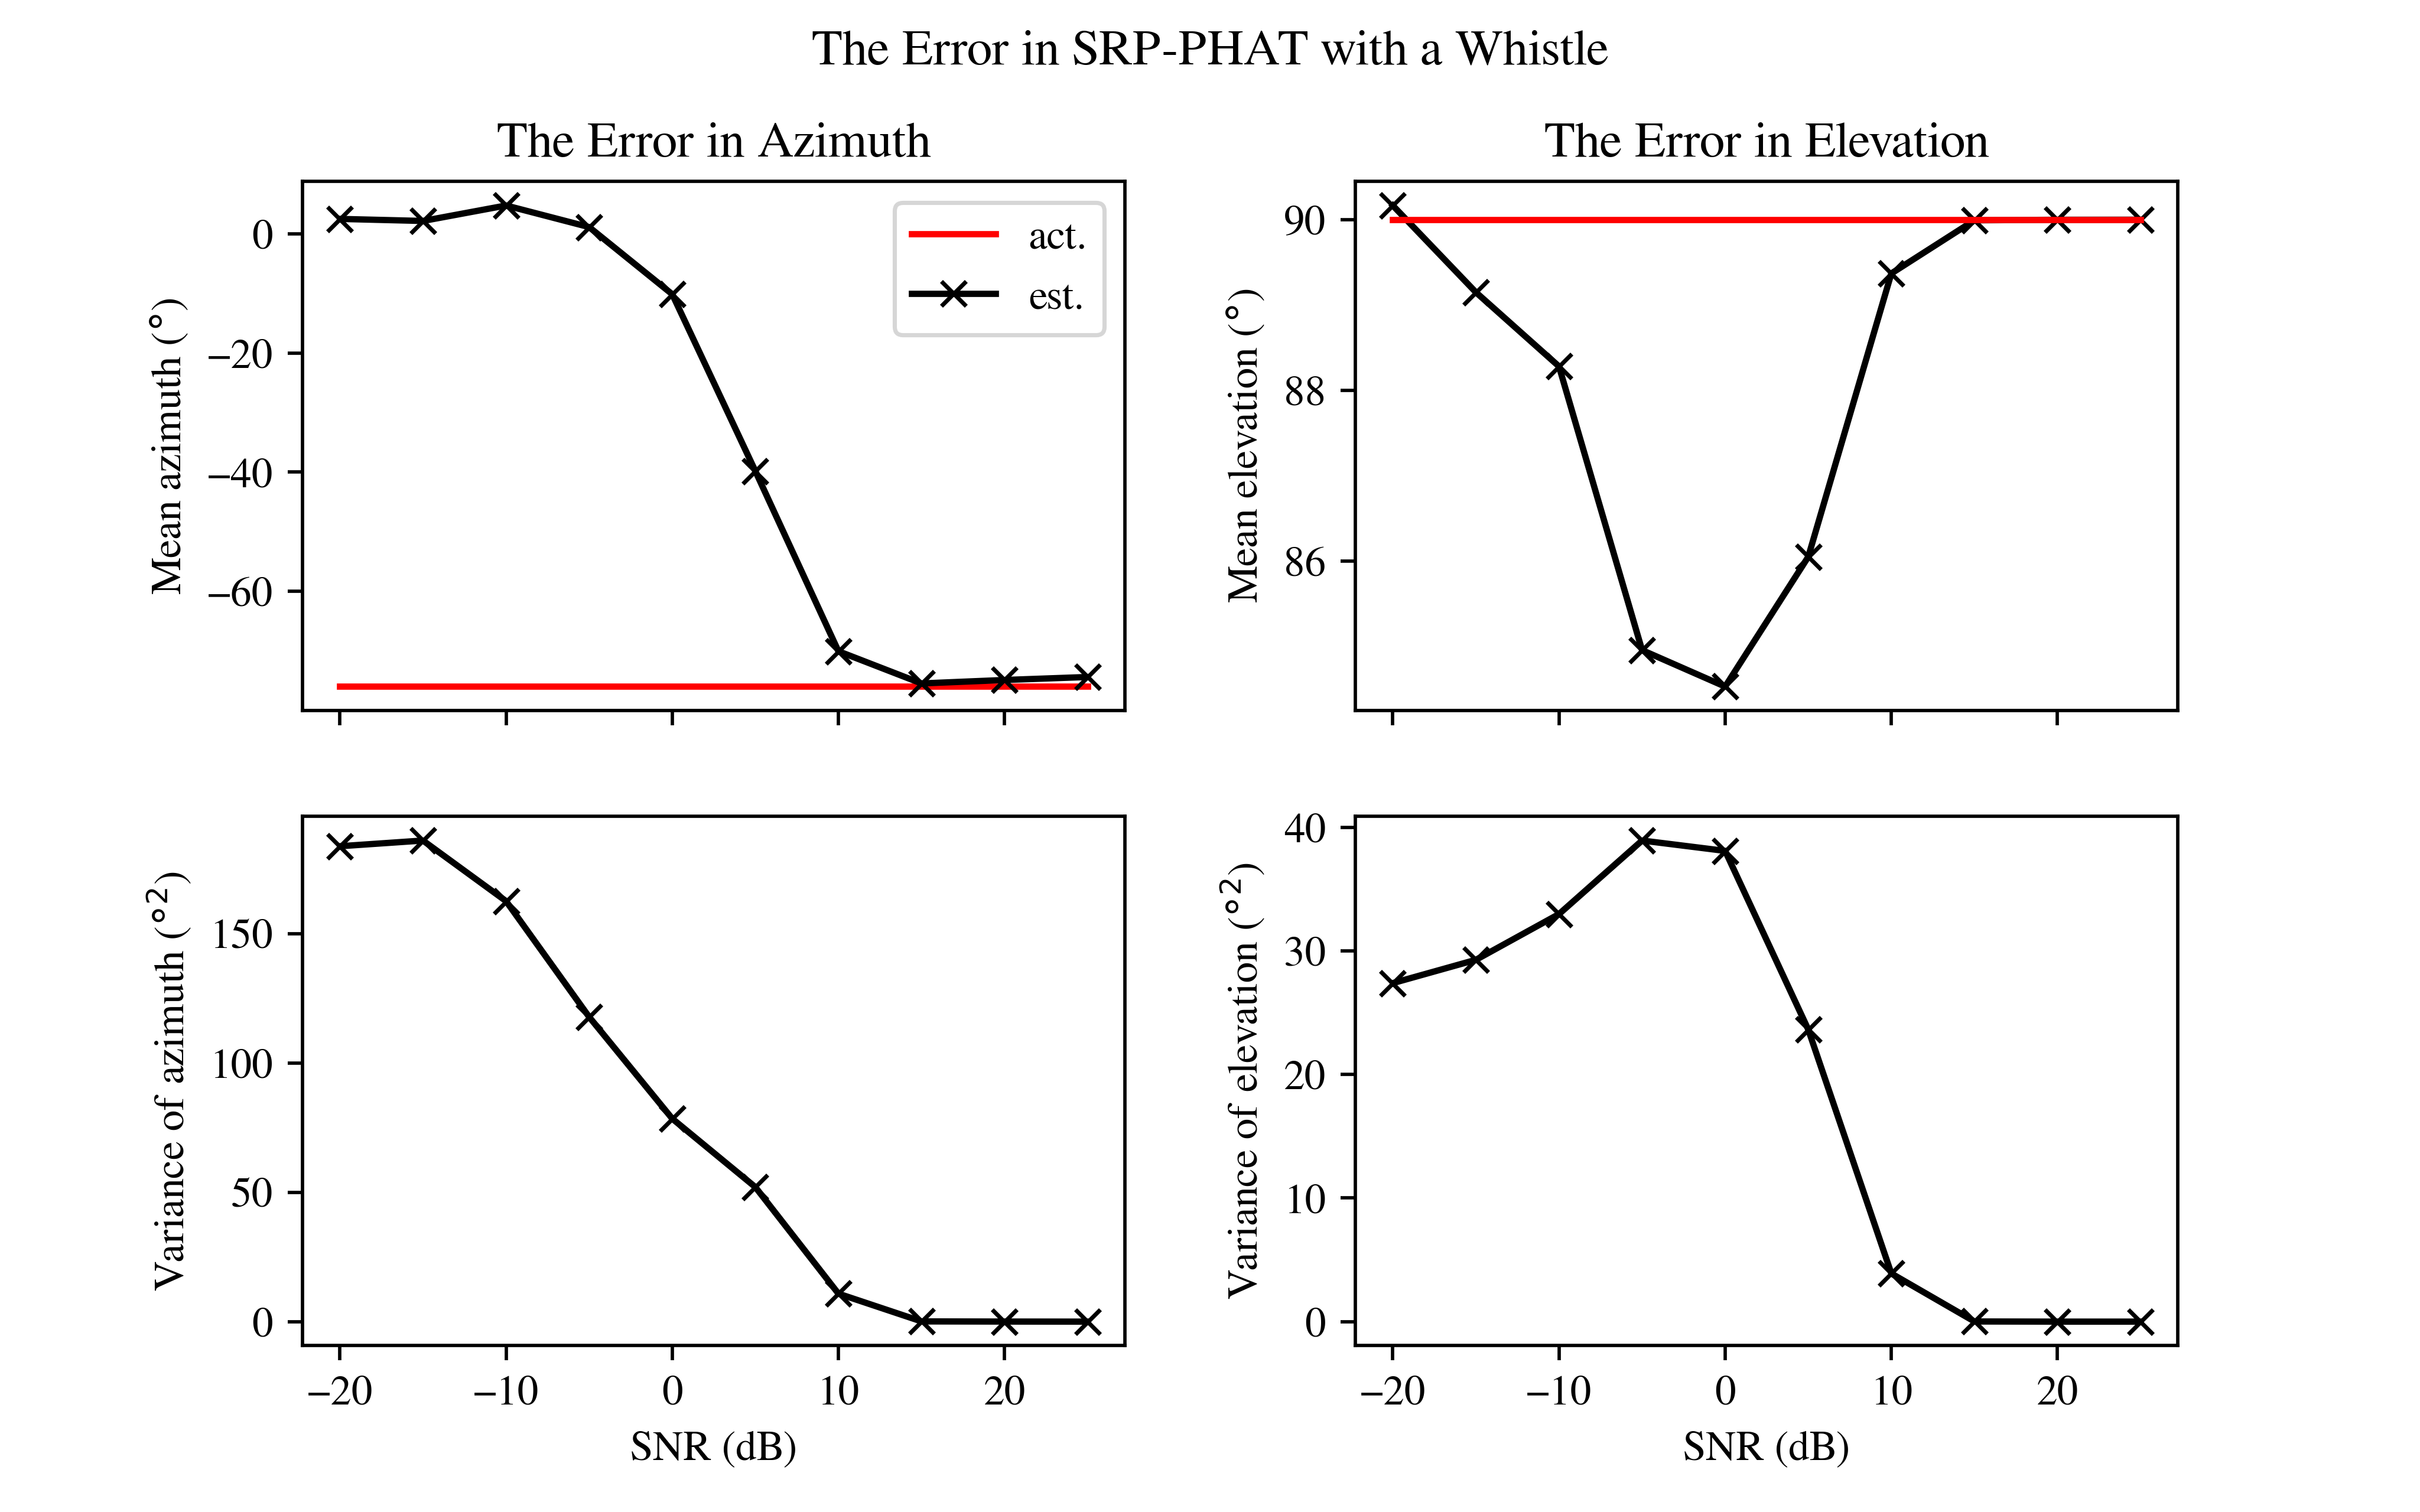
\includegraphics[width=0.9\textwidth]{../Python/srp_phat/noise/whistle/plots.png}
\centering
\caption{The statistical performance of the estimated direction is plotted against noise with a whistle as the source.}
\label{fig:srp_phat_noise_whistle}
\centering
\end{figure}

With a broadband signal like a clap, it was seen from these results that the method was fairly robust against noise since there is very little variance in both the estimated azimuth and elevation even though it did grow as the noise was increased. Indeed, the mean of the estimated azimuth did have some bias initially which shifted as the noise increased as seen in Figure-\ref{fig:srp_phat_noise_clap}. However, this can simply be explained by the fact that the spherical grid introduces some discrete resolution. In fact, the same authors in the two cited papers \cite{valin_localization_2004} \cite{valin_robust_2007} suggest a smaller finer search grid after estimating the direction from the coarse grid. However, this was optional step was omitted in this simulation to highlight the basic performance of the SRP-PHAT method.

On the other hand, the performance was much worse with a narrowband signal like a whistle with both the bias and the variance much larger. The system seemed to break down dramatically for noise past a SNR of 15 \si{dB}. 

\subsubsection{Visualisation of the Energy-Map} \label{Visualisation_of_the_Energy_Map}

A worthwhile endevour was to plot the spherical energy-map to get a better insight into how the method works and the effect from noise. This was done by plotting the energy two-dimensionally against the azimuth and the elevation as the axes. Granted, this gave a distorted view towards the top and bottom edge of the map\footnote{In fact, this is even much like many conventional projections of the Earth on a flat map}. Nevertheless, this drawing of the energy-map was accurate around the middle where the source lied.

\begin{figure}[H]
\includegraphics[width=0.9\textwidth]{../Python/srp_phat/noise/clap/map.png}
\centering
\caption{The energy-map of the SRP-PHAT beamformer is drawn with a clap as the source.}
\label{fig:srp_phat_noise_map_clap}
\centering
\end{figure}

\begin{figure}[H]
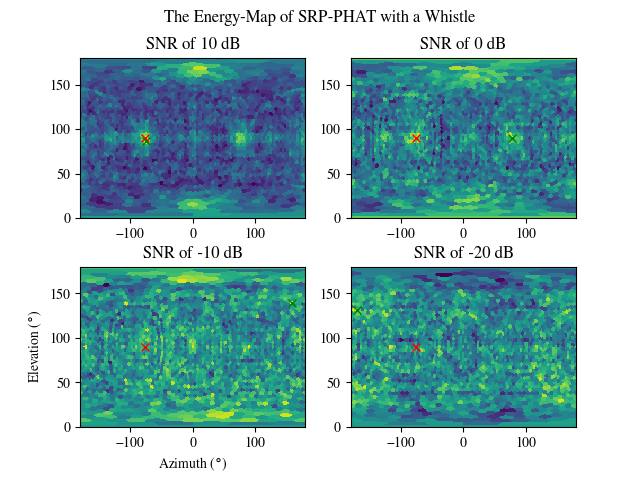
\includegraphics[width=0.9\textwidth]{../Python/srp_phat/noise/whistle/map.png}
\centering
\caption{The energy-map of the SRP-PHAT beamformer is drawn with a whistle as the source.}
\label{fig:srp_phat_noise_map_whistle}
\centering
\end{figure}

For low noise, there was a very thin and tall peak where the source lied as seen in Figure-\ref{fig:srp_phat_noise_map_clap}. However, as the noise increased, the peak became wider, whilst the rest of the map became more diffused and noisy. This shows how the variance worsened and even how the mean drifted against rising noise since the peak on the energy-map behaves like a probability-distribution. In fact, the whole energy-map is much like a probability-density function.

The effect of noise with a narrowband signal can be seen more easily; the noisy background as much worse in Figure-\ref{fig:srp_phat_noise_map_whistle}.

In some of the maps in Figure-\ref{fig:srp_phat_noise_map_clap}, the side-lobes often associated with beamforming in the literature can be seen; these are seen as subtle curved lines coming from the peak as well as shorter secondary peaks in other directions. Luckily, these do not seem to be too high at least for this geometry.

The energy-map also showed how multiple simultaneous sources could be localised since they would show up as two distinct peaks.

\subsubsection{Discussion}

Indeed, the SRP-PHAT seemed more robust to noise than the other TDOA-based method for the rectangular pyramid array by \cite{chen_sound_2019} although it could not estimate the distance. It did however seem to take twice as long to estimate one direction in the Python simulations; this may be because the method needs to compute for many discrete directions on a search-grid. This apparent slowness can be lessen by pruning obselete directions in the grid, e.g. directly below the array.

The SRP-PHAT was very poor for a narrowband signal such as a whistle. However, this was somewhat expected since it was known that the PHAT worked worse with narrowband signals \cite{valin_localization_2004} \cite{valin_robust_2007}. This may be considered the worst kind of sound and thus set a lower bound of performance; other kinds of sound should fare better. Even still, this can be fine-tuned with some parameters like the sampling rate, the frame-length, the modified spectral weighting. 

\section{Further Study into SRP-PHAT}

Given the method used in some paper \cite{valin_localization_2004}\cite{valin_robust_2007}\cite{manamperi_drone_2022}\cite{salvati_power_2019}\cite{basiri_-board_2016}, a further study in its parameters such as sampling frequency was needed before committing to a final design. These parameters were especially important for this project since they dictate the level of computation and memory on an embedded design. This study would give insight into the design and choice of such parameters.

\subsection{Experimental Method}

For this set of simulations, the same room was tested as before, but the array was 91.2 \si{mm} wide. This was the width of a cube that could fit inside the NUgus' spherical head and thus would give a rough estimate of the chosen geometry. Furthermore, the SNR was kept at 0 \si{dB} since this would be a rough middle ground for the expected noise.

For the sound, a recording of claps taken in an anechoic chamber was used \cite{noauthor_handclaps_2005}. As seen before, this would be a broadband signal and would thus be considered a reliable sound to localise with SRP-PHAT.

For each independent variable, 10,000 runs of the same simulation were done but with pseudo-random results. Thereby, the mean and the variance of the output were recorded; the former would thus show the accuracy, and the latter would show the precision and the repeatability.

To further help visualise the effect, maps of the beam's energy over the spherical search grid were drawn along with the plots.

\subsection{Effect of the Sampling Frequency}

As seen before, the sampling frequency can affect the overall accuracy of the GCC-PHAT. Furthermore, a slower sampling rate can ease computation and the time-length of a frame. Here, the sampling frequency was varied from 16 to 120 \si{kHz}, whilst the SNR was kept at 10 \si{dB}, and the frame's length was kept at 1024.

Since the same audio-file was tested which had an original sampling frequency of 96 \si{kHz}, it had to be either downsampled or upsampled. This was done using the SciPy library in Python.

As seen in Figure-\ref{fig:mm_frequency_map_clap}, the correlation between the accuracy and the sampling frequency was somewhat non-linear. In addition, the variance for both worsened as the sampling frequency decreased past 48 \si{kHz}, but not dramatically.

\begin{figure}[H]
\includegraphics[width=0.9\textwidth]{../Python/main_method/frequency/clap/plots.png}
\centering
\caption{The statistical performance of the estimated direction was plotted against the sampling frequency with a clap as the source.}
\label{fig:mm_frequency_plots_clap}
\centering
\end{figure}

Furthermore, as seen in Figure-\ref{fig:mm_frequency_map_clap}, the beam was considerably wider for a sampling frequency of 24 \si{kHz} but was still distinct against the background.

\begin{figure}[H]
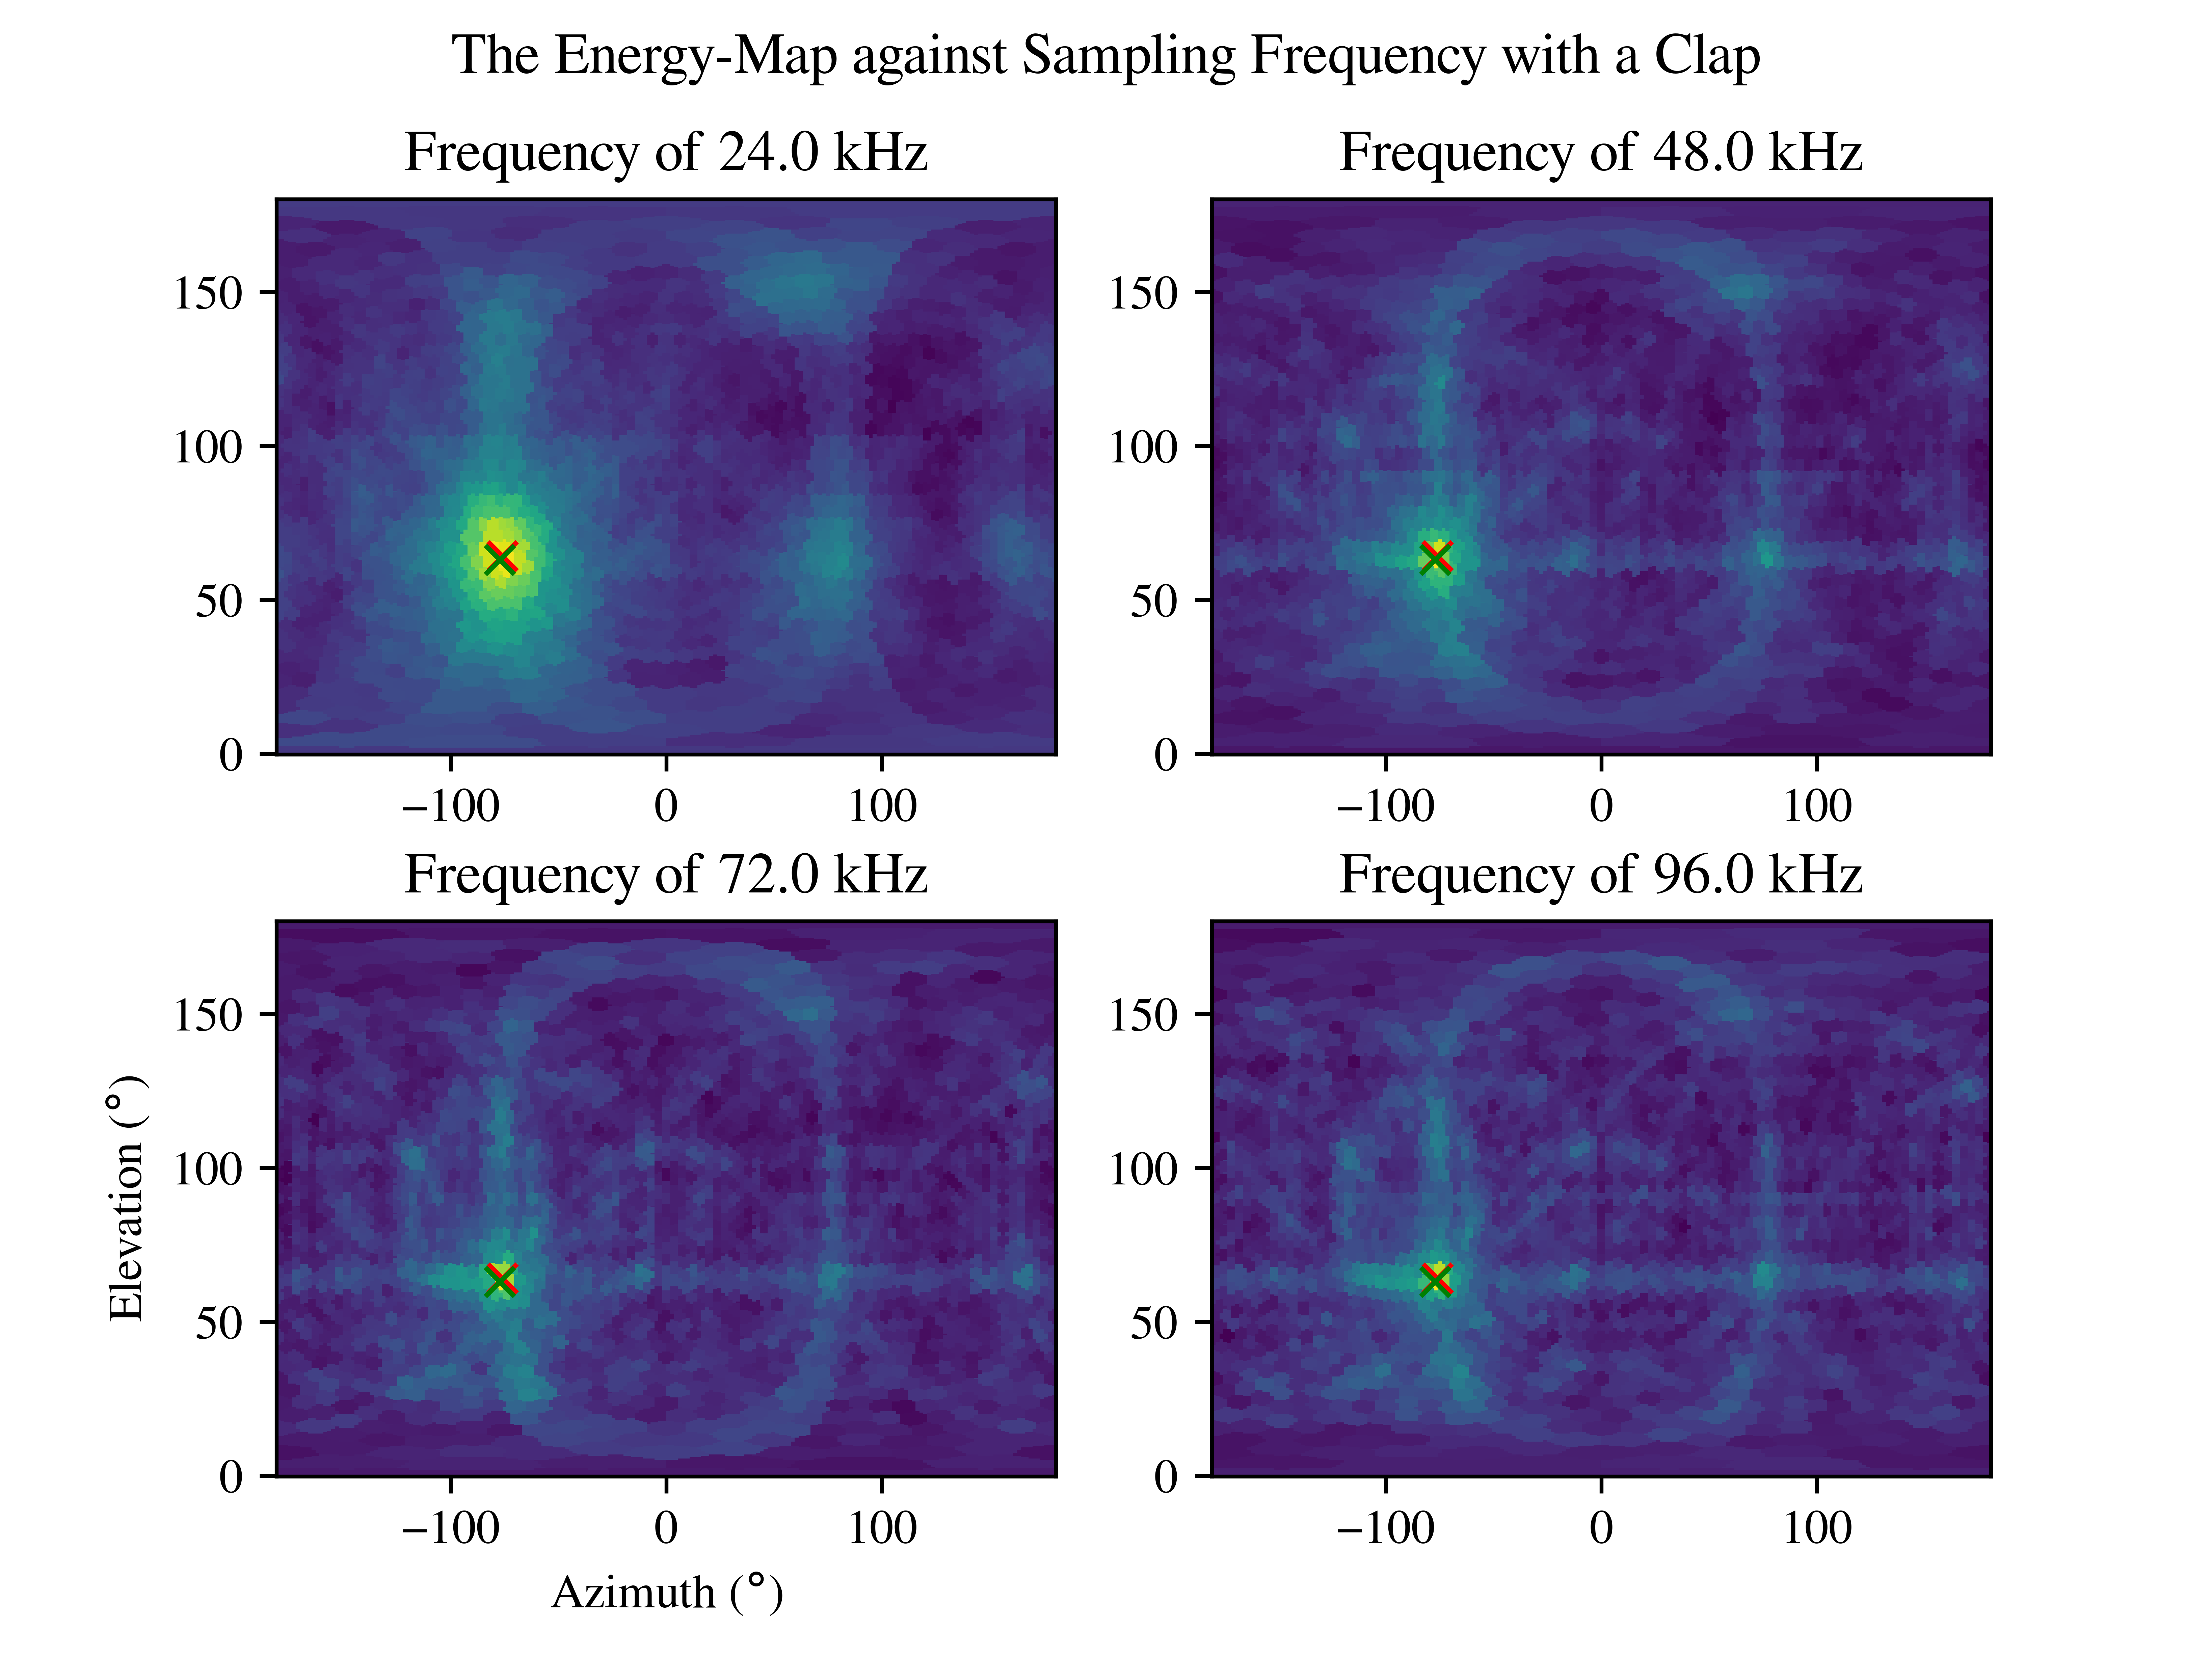
\includegraphics[width=0.9\textwidth]{../Python/main_method/frequency/clap/map.png}
\centering
\caption{The energy-map of the proposed beamformer was drawn with a clap as the source.}
\label{fig:mm_frequency_map_clap}
\centering
\end{figure}

\subsection{Effect of the Frame's Length} \label{Effect_of_the_Frames_Length}

The frame's length can also affect computation and more specifically the needed memory to store buffers, vectors, etc. Thus, a range of common frame-lengths from 64 to 2048 were tested, whilst the SNR was kept at 10 \si{dB}. Furthermore, the sampling frequency was kept at 24 \si{kHz}.

As seen in Figure-\ref{fig:mm_length_plots_clap}, the accuracy, i.e. the mean, for both the azimuth and the elevation worsened a lot for frame-lengths of 64 and 128. Therefore, the minimum frame-length would be 256 samples, at least for an SNR of 10 \si{dB}.

\begin{figure}[H]
\includegraphics[width=0.9\textwidth]{../Python/main_method/length/clap/plots.png}
\centering
\caption{The statistical performance of the estimated direction was plotted against the sampling frequency with a clap as the source.}
\label{fig:mm_length_plots_clap}
\centering
\end{figure}

The maps in Figure-\ref{fig:mm_length_map_clap} show that beam's energy was consistent for lengths of 128, 512, and 2048 but worsened a bit for that of 64. Interestingly, the beam of which made a strange traingular shape with lots of non-linear anamolies.

\begin{figure}[H]
\includegraphics[width=0.9\textwidth]{../Python/main_method/length/clap/map.png}
\centering
\caption{The energy-map of the SRP-PHAT beamformer was drawn with a clap as the source.}
\label{fig:mm_length_map_clap}
\centering
\end{figure}

\subsection{Rudimentry Analysis of Computation}

To make sure that the proposed algorithm was feasible to run real-time on an embedded system, the needed computation had to be analysed. This was mostly difficult to predict since the number of needed clock-cycles is hard to predict for instructions let alone floating-point operations. This is since CPUs and instruction-sets vary especially if they are pipelined.

However, the number of floating-point operations were estimated using a simple Python script that used recursive functions to count the number of floating-point operations for a given high-level function, e.g. FFT. Also, by counting floating-point operations, this kept the analysis general for any processor, regardless of the architecture or the instruction-set.

The algorithm was split up into three main tasks:
\begin{itemize}
	\item computing the FFT, the magnitude of which, and the complex conjugate of which,
	\item computing the GCC for all pairs where there were 28 given an array of eight microphones,
	\item and computing the beam for each direction.
\end{itemize}

The result of which was that a frame of 1024 samples would need about 3.49 million floating-point operations. If the sampling frequency was 24 \si{kHz}, this would need about 81.8 MFLOPS.

Assuming that the processor's clock-frequency would be 200 \si{MHz} and that a floating-point operation would need ten clock-cycles, then the maximum number of floating-point operations within a frame would be:
\begin{equation}
200 \si{MHz} \times \frac{1024}{24 \si{kHz}} / 10 = 853 \text{ thousand}
\end{equation}

Most of the computation seems to be the FFT, particularly the inverse FFT done 28-fold for each pair's GCC-PHAT. Given that FFT is generally considered to take $F \log_2(F)$ complex additions and $F/2 \log_2(F)$ complex multiplications. Assuming that a complex addition is two real additions, a complex multiplication is four real multiplications and two real additions, then this inverse FFT for the GCC-PHAT of all 28 pairs would take:
\begin{equation}
\begin{split}
&28 \cdot \left( 1024 \log_2(1024) \cdot 2 \right. \\
&\left. + \frac{1024}{2} \log_2(1024) \cdot (4+2) \right) \\
&= 574 \text{ thousand floating-point operations}
\end{split}
\end{equation}
% may need citation

However, this analysis does not take hardware-accelerated FFT into account. As long as the chosen processor has some hardware-acceleration for FFT, then the system may be feasible to run real-time. Again, this analysis was meant to give a rudimentary prediction of the needed computation.

\chapter{Proposed System}

After some thorough analysis of two literature-examples and of a common technique namely SRP-PHAT\cite{valin_localization_2004}\cite{valin_robust_2007}\cite{manamperi_drone_2022}\cite{salvati_power_2019}\cite{basiri_-board_2016}, a sound-source-localisation algorithm along with some parameters was proposed for this project which was based on SRP-PHAT. Furthermore, a slightly novel approach was taken to filter out spurious results, see Section-\ref{Confidence}. Thus, this chapter explains the main structure and design of the algorithm.

\section{Algorithm}

Because of the embedded nature of the system, the algorithm was kept relatively simple. A number of optimisations were taken thereon such as the FFT and the magnitude which were computed once for each microphone. This algorithm was to be done on one frame of samples at a time. The TDOAs $\tau_{gij}$ for each pair $i,j$ and for each direction $g$ was computed once since it is constant and independent of the data.

\begin{algorithm}[H]
\caption{The proposed algorithm based of SRP for the prototype}
\label{alg:proposed_algorithm}
\begin{algorithmic}
	\For{every $i$-th microphone where $i = 0, ..., 7$}
		\State $x_i$ is the frame of samples
		\State $X_i \gets$ the FFT of $x_i$
		\State $\lvert X_i \rvert \gets$ the magnitude of $X_i$
		\State $X_i^* \gets$ the complex conjugate of $X_i$
	\EndFor
	
	\For{every $ij$-th pair of microphones where $i = 0, ..., 7$ and $j \neq i$}
		\State Compute the GCC-PHAT as 
		$R_{ij} \gets \mathfrak{F}^{-1} \left( \frac{X_i X_j^*}{\lvert X_i \rvert\lvert X_j \rvert} \right)$
	\EndFor
	
	\For{every $g$-th direction in the spherical search-grid}
		\State Compute the beam's energy as 
		$E\gets \sum_{i=0}^{M} \sum_{j=0}^{M} R_{ij}(\tau_{gij})$
		\If{$E \geq E_{\text{max}}$}
			\State $g_{\text{max}} \gets g$
			\State $E_{\text{max}} \gets E$
		\EndIf
	\EndFor
	
	\State Get the etimated direction of the sound-source as $\vec{u} = \vec{u}_g$
\end{algorithmic}
\end{algorithm} 

Here, the same spherical search-grid of 2562 directions was used as in \cite{valin_localization_2004} and \cite{valin_robust_2007} although an additional finer grid was not. This was mostly chosen because of convenience since a Python function was already made that tesselated such a grid.

\section{Chosen Parameters}

Furthermore, a frame of 1024 was used since it seemed to be the most commonly used in the literature, and it seems to show good performance in Section-\ref{Effect_of_the_Frames_Length}.

A sampling frequency of 24 \si{kHz} was used mostly because of firmware and computational reasons later on in this thesis, see Section-\ref{Computation_and_Timing}. Originally, a rate of 48 \si{kHz} was going to be used, but real-time constraints later on in the design of the firmware pushed it to be lower.

\section{Confidence} \label{Confidence}

From the energy-maps in Section-\ref{Visualisation_of_the_Energy_Map}, it was taken into mind that the worse the noise was, the shorter the beam was, like a hill so to speak. This was used to draw therefrom an estimated confidence. Thus, a simple value for confidence was  taken as the difference in the beam's energy and the standard deviation of the rest of the energy-map.
\begin{equation}
\mathfrak{C} = E_{\text{max}} - \sqrt{\sum_{g=0}^{G} \frac{(E_g-\bar{E})}{G-1}}
\end{equation}
where $\bar{E}$ is the mean of all the energies $E_g$.

This should need little computation since it is adding over 2562 floating-point values. It would also improve the robustness to noise especially narrowband signals. It is known from Section-\ref{SRP_PHAT} that a narrowband signal like a whistle is very hard to localise with noise. However, the fading edges of the whistle's burst have wider bands of frequencies. If the confidence $\mathfrak{C}$ of the estimated direction $E_{\text{max}}$ is more than a chosen threshold, then the estimations of the frames with the fading edges can be used and the spurious estimations of the fames in the middle of the whistle's tone can be ignored. Thus, narrowband signals can still be more reliably estimated therefrom.

\section{Chosen Geometry}

As for the array itself, its geometry and dimensions were mostly confined to the dimensions of the NUgus' spherical head which is 158 \si{mm} in diameter. A cube, or at least a rectangular geometry, was chosen since it was the most straightforward and the most common in the literature, especially in \cite{valin_localization_2004} and \cite{valin_robust_2007}.

The first option was to fit a cube in the sphere such that its vertices were on the surface. This would be akin to embedding microphones on the surface of the NUgus' head such that they formed a cube. Such a method would need modifications to the head such as drilled holes.

However, the head itself is made up of 3D-printed parts, and the sides of the head can be taken off which leaves a wide opening on both sides as seen in Figure-\ref{fig:geometry_head}. In fact, the sides are purely aesthetic and are often left off during competitions, events, etc. so that the cameras can be easily accessed.

\begin{figure}[H]
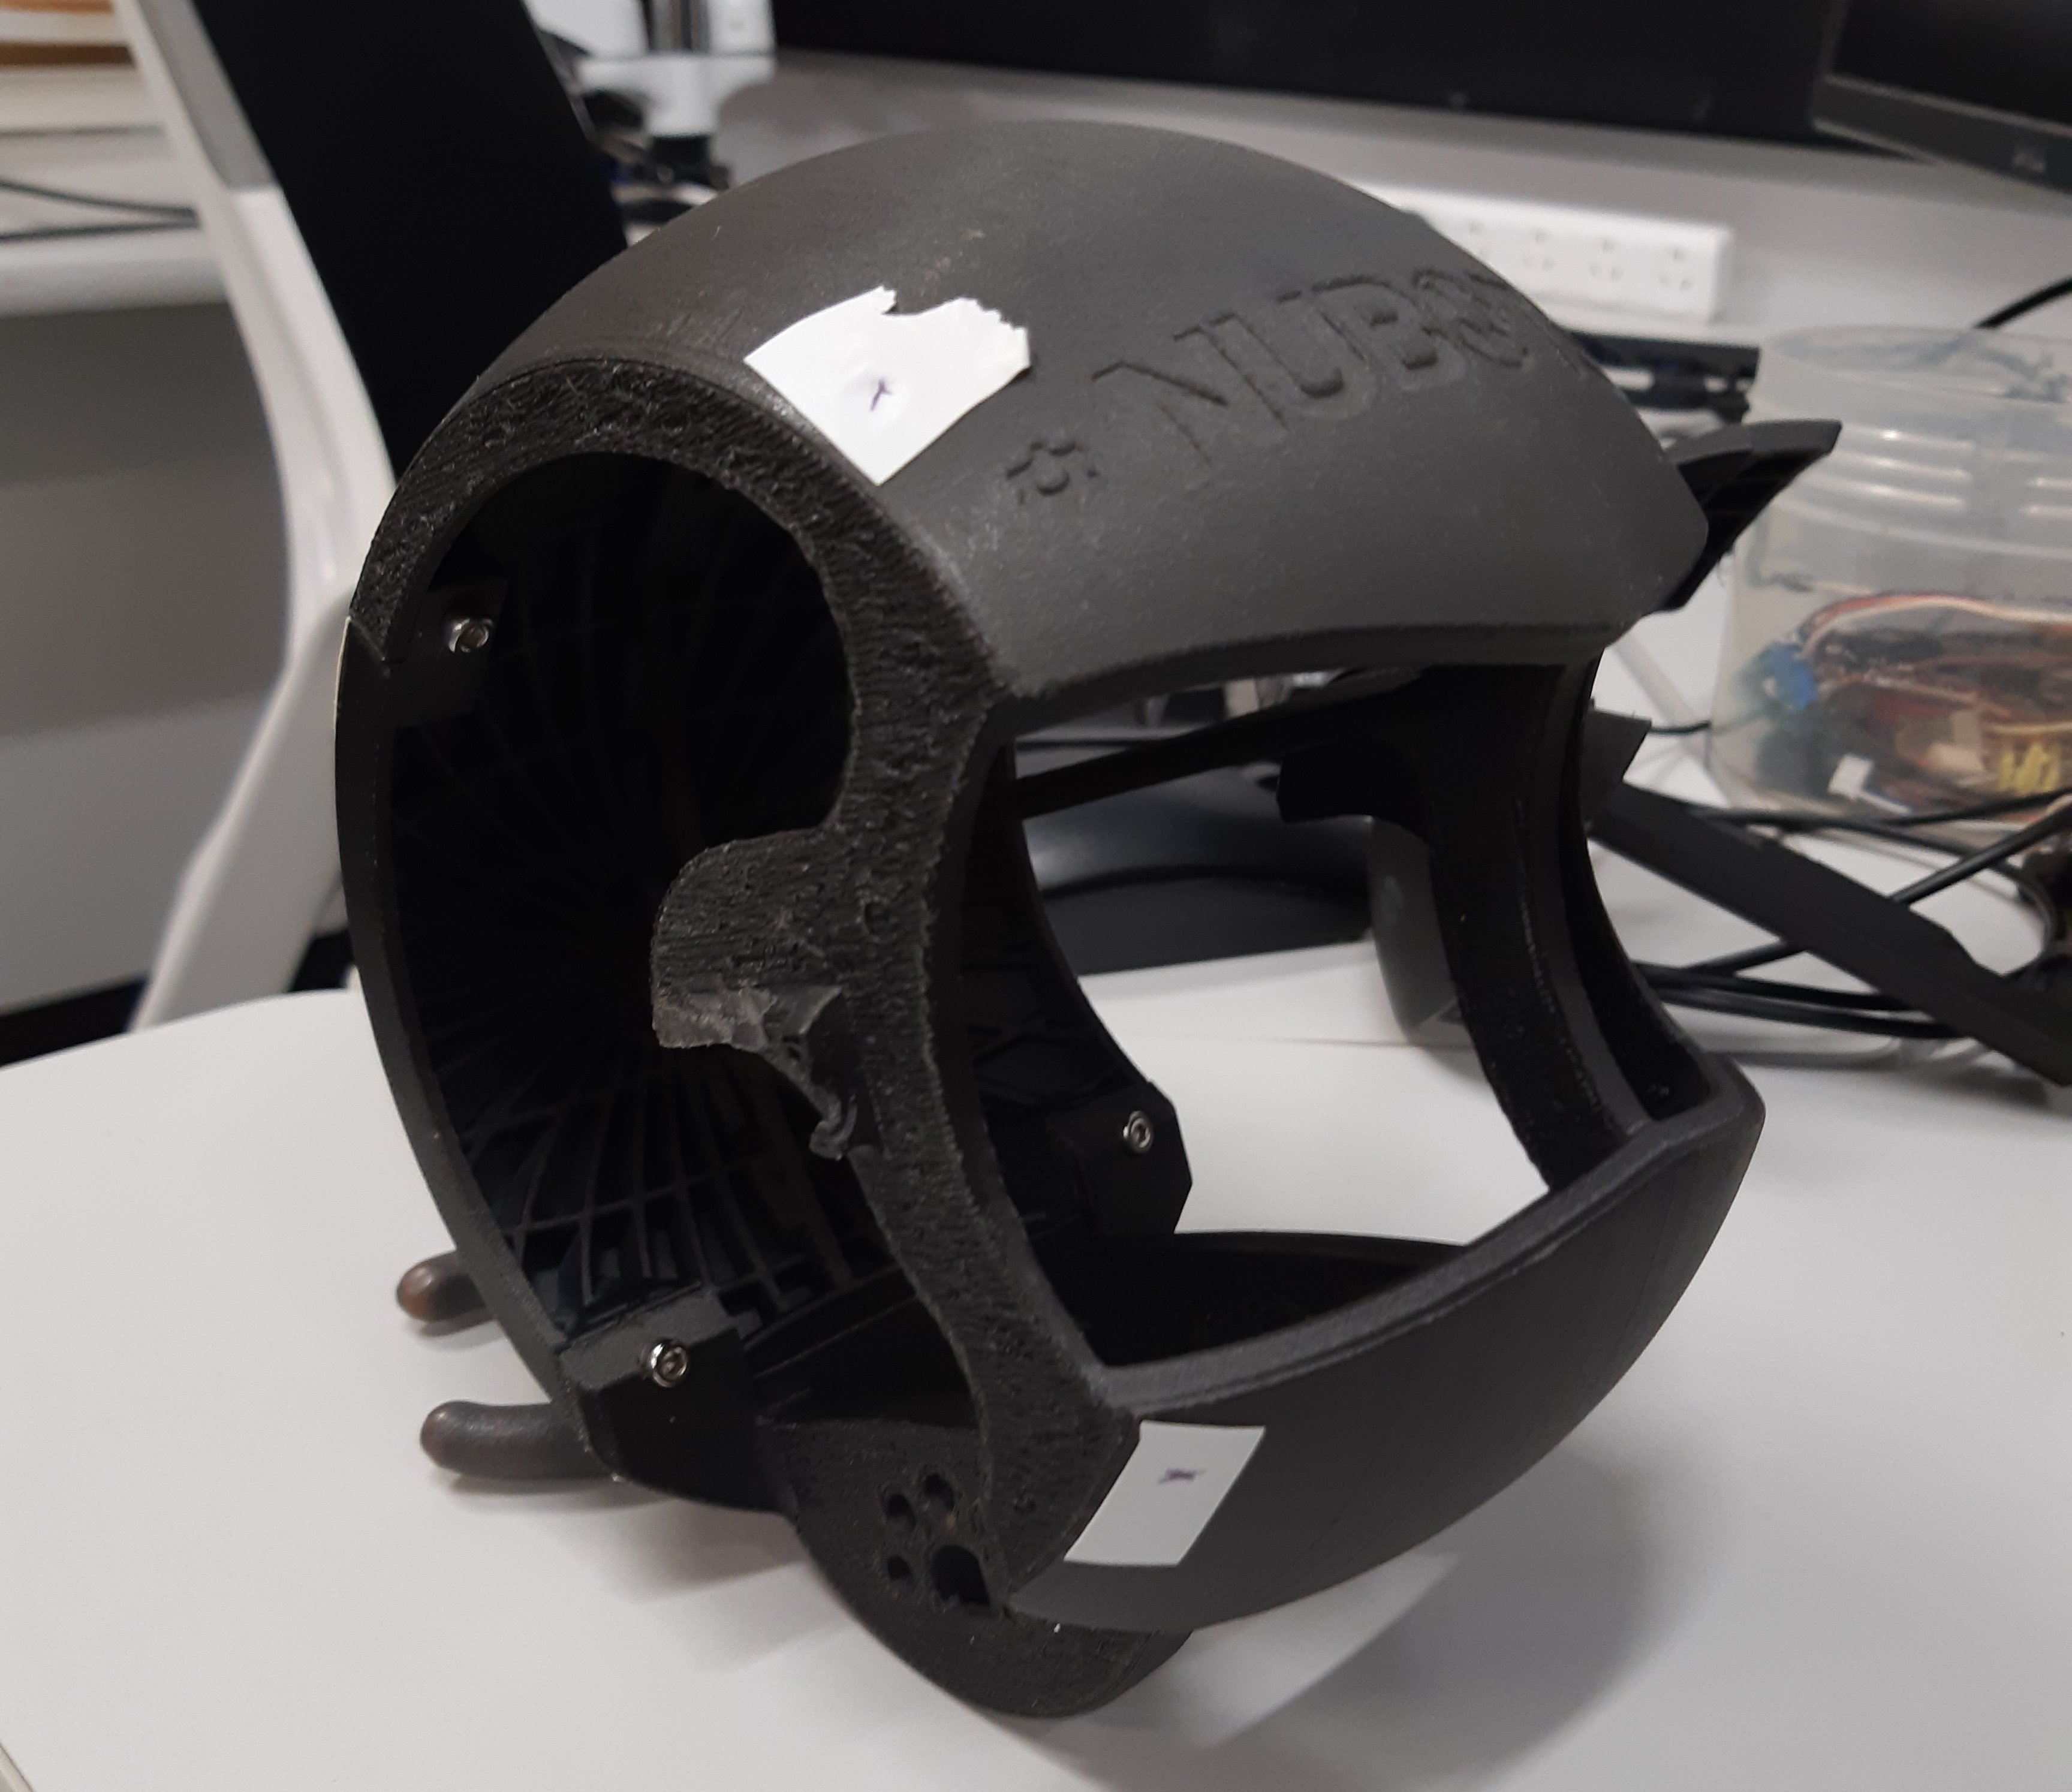
\includegraphics[width=0.9\textwidth]{./photo_head.jpg}
\centering
\caption{The 3D-printed head of the NUgus robot with the side-plates taken off.}
\label{fig:geometry_head}
\centering
\end{figure}

Therefore, the second option is to take advantage of this and have a slightly wider rectangular array so that the four microphones on each side can more comfortably sit inside these openings. Furthermore, the openings allow the microphones to have more line of sight, improving the robustness to delays relating to the head-transfer.

\chapter{Simulation of the Proposed System} \label{Simulation_of_the_Proposed_System}

A final simulation of the proposed system was done to make sure of its feasibility. The biggest factor was the different array which was somewhat smaller than the simulated examples from the literature-review as well as the sampling frequency. From here, this chapter talks about the methodoloy and the results. Again, all of the code is available in in this project's GitHub repository\footnote{Note that there may be commits afterwards.}: \url{https://github.com/Claegtun/fyp-nubots-ssl}.

\section{Experimental Method}

As before, the array under test was put in the centre of the room; that is 1 \si{m} off the floor in the centre of a closed room 10 \si{m} wide, 10 \si{m} long, and 3 \si{m} high. The array was also oriented to be in line with the room. Given that the origin was in one bottom corner of the room, the coordinates of the array's centre were $(5,5,1)$. Furthermore, an absorption factor of 0.5 was used for the walls. This gave RIRs similar to that seen in Figure-\ref{fig:pyramid_robot_noise_rir} and an estimated reverberation-time at 60 \si{dB} of 84.8 \si{ms}. This would roughly emulate a large indoor office-space with moderate reverberation.

Since the exact array was not know at this stage, the array was assumed to be a cube 91.2 \si{mm} wide. This was the width of a cube that could fit inside the NUgus' spherical head and thus would give a rough estimate of the chosen geometry.

For the sound, two kinds were tested; first, a recording of claps taken in an anechoic chamber was used \cite{noauthor_handclaps_2005}; secondly, a recording of a whistle. The former sound models a typical broadband signal, whilst the latter models a typical narrowband signal. These sounds were resampled to 24 \si{kHz} to ensure a consistent analysis.

For each independent variable, 10,000 runs of the same simulation were done but with pseudo-random results. Thereby, the mean and the variance of the output were recorded; the former would thus show the accuracy, and the latter would show the precision.

To further help visualise the effect, maps of the beam's energy over the spherical search grid were drawn along with the plots.

\section{Performance against Noise} \label{Performance_against_Noise}

The source was set at $(5.5,3,2)$ to give an arbitrary but realistic direction, e.g. not straight ahead. Overall, ten levels of noise were simulated for which, i.e. SNRs from -20 to 25 \si{dB}.

As seen in Figure-\ref{fig:mm_noise_plots_clap} and -\ref{fig:mm_noise_plots_whistle},the accuracy for both azimuth and the elevation stayed within the expected resolution. For a clap, both the accuracy and the precision worsened dramatically at an SNR of -20 \si{dB}; for a whistle, they worsened for an SNR less than -5 \si{dB}.

\begin{figure}[H]
\includegraphics[width=0.9\textwidth]{../Python/main_method/noise/clap/plots.png}
\centering
\caption{The statistical performance of the estimated direction was plotted against the noise with a clap as the source.}
\label{fig:mm_noise_plots_clap}
\centering
\end{figure}

\begin{figure}[H]
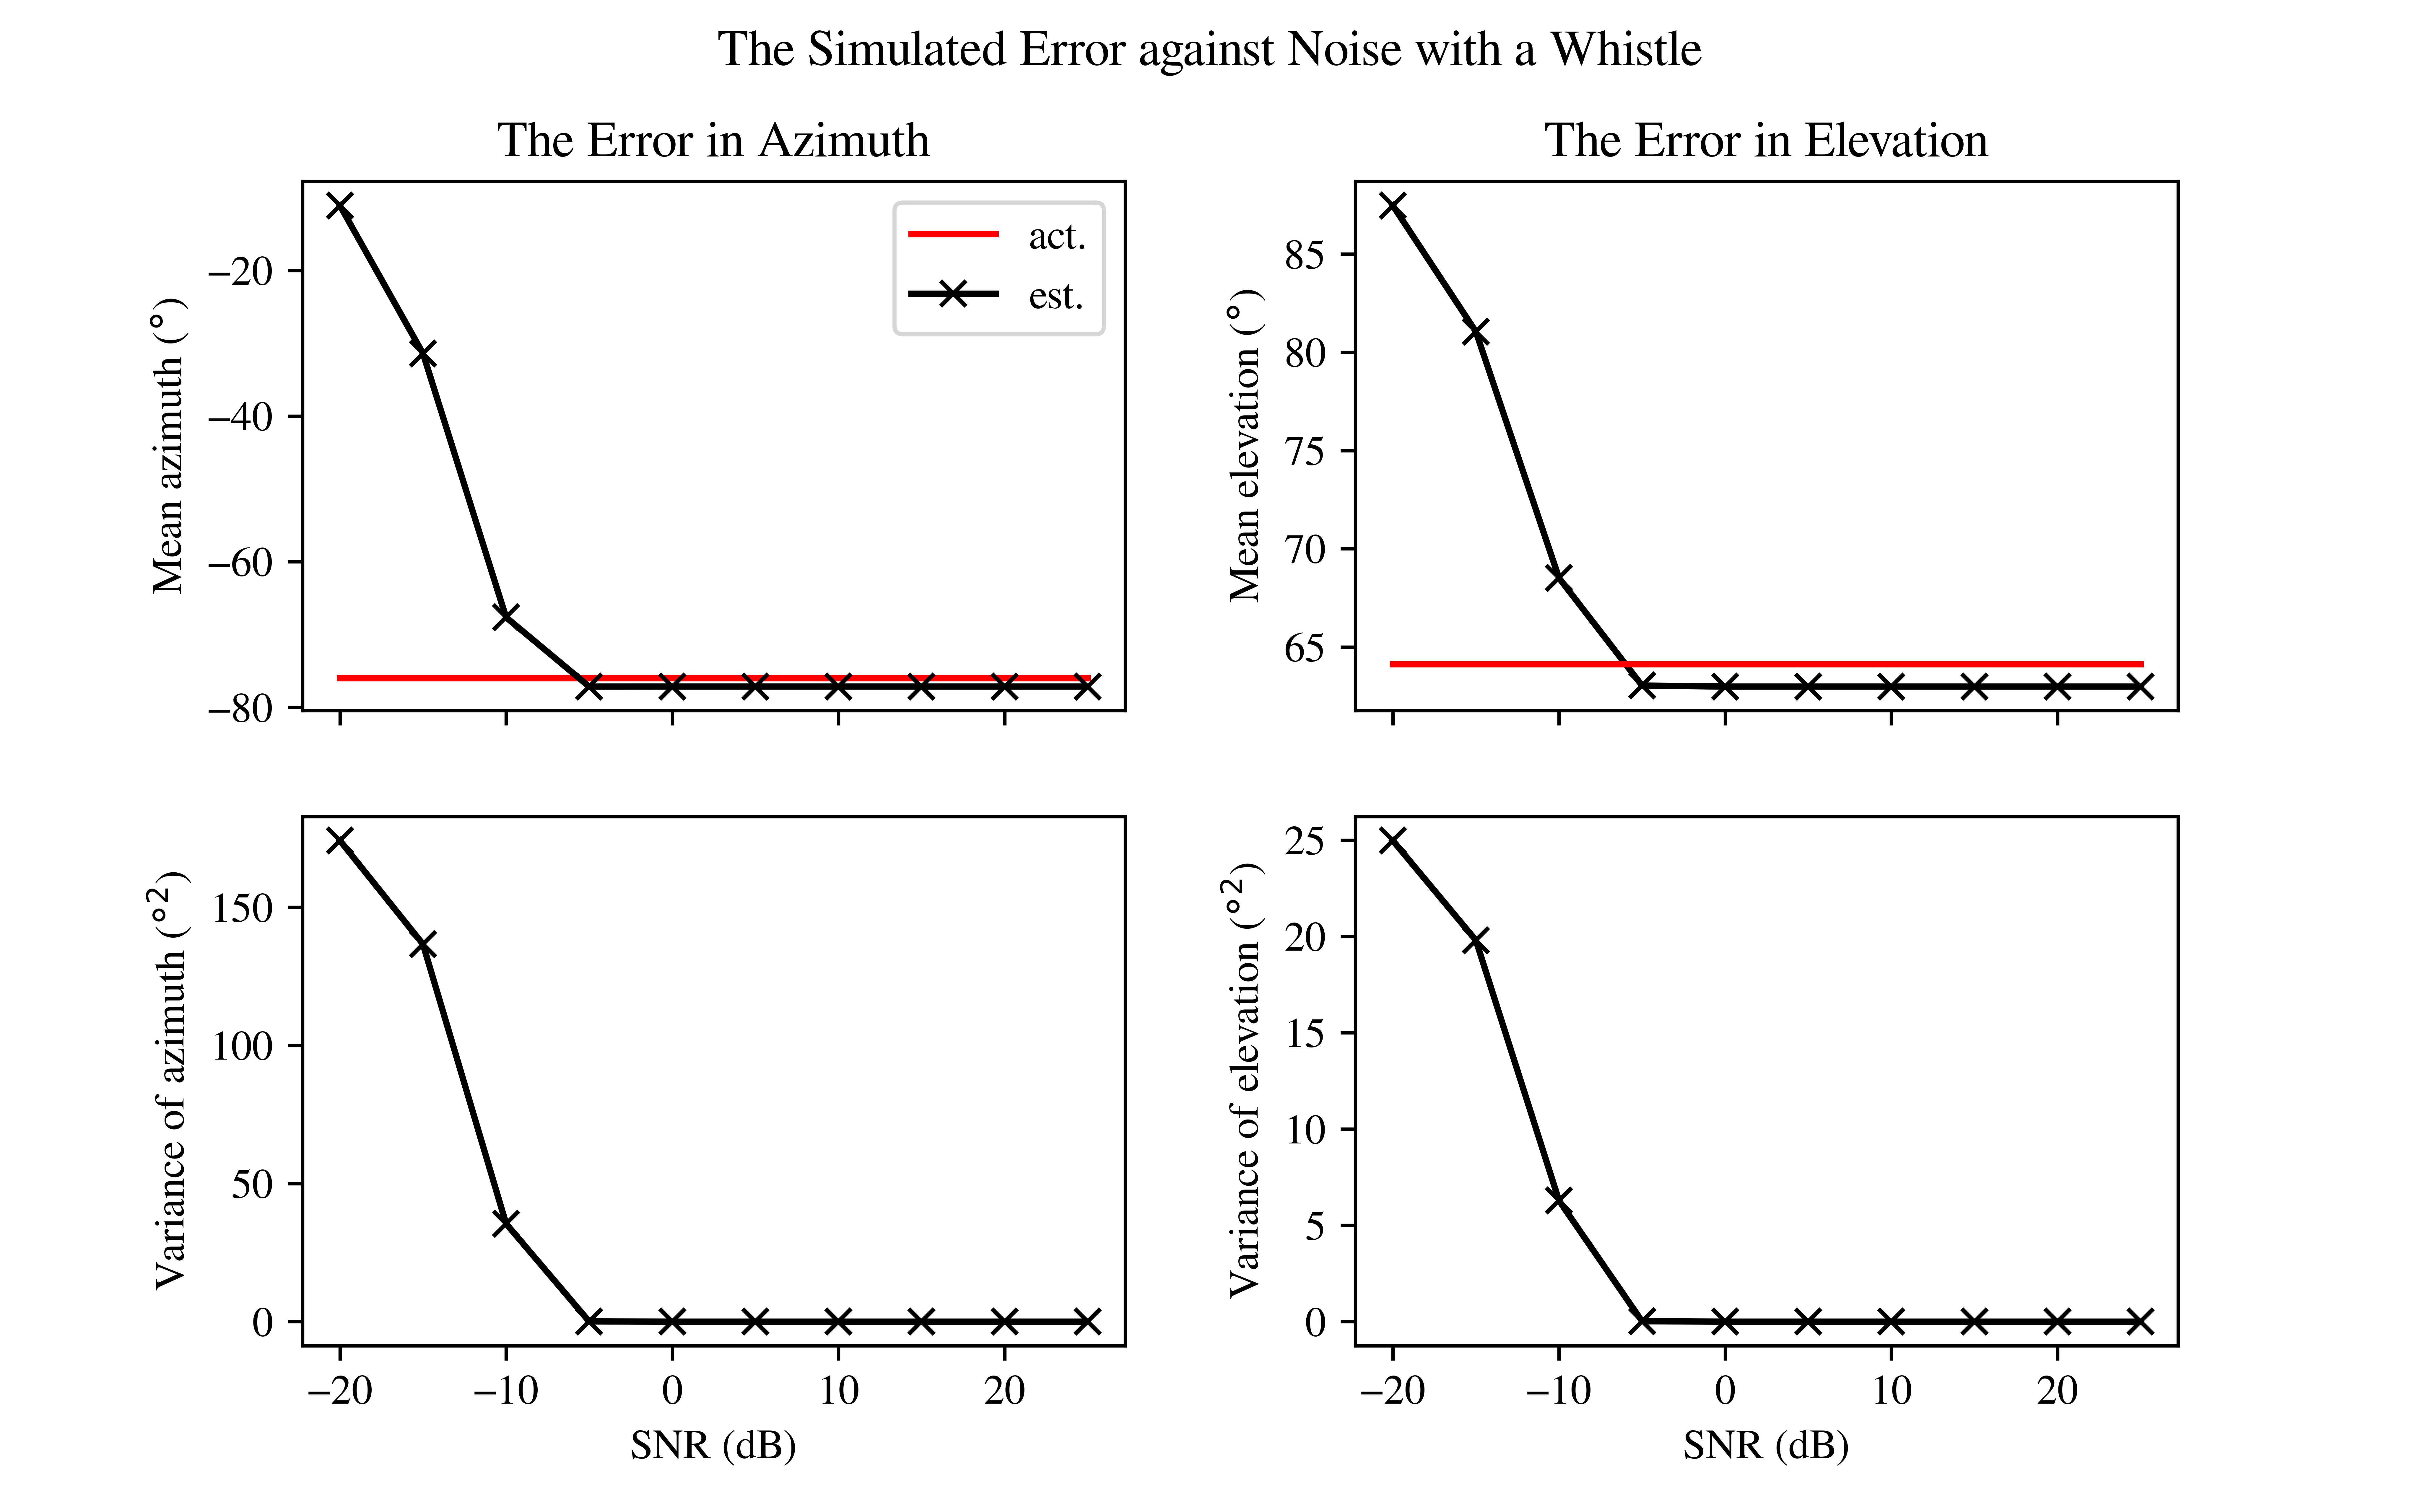
\includegraphics[width=0.9\textwidth]{../Python/main_method/noise/whistle/plots.png}
\centering
\caption{The statistical performance of the estimated direction was plotted against the noise with a whistle as the source.}
\label{fig:mm_noise_plots_whistle}
\centering
\end{figure}

In Figure-\ref{fig:mm_noise_map_clap} and -\ref{fig:mm_noise_map_whistle}, show that beam became wider and shorter against the background as the noise grew. In particular for the SNRs of -10 and -20 \si{dB}, the beam was completely missing amongst the noise.

\begin{figure}[H]
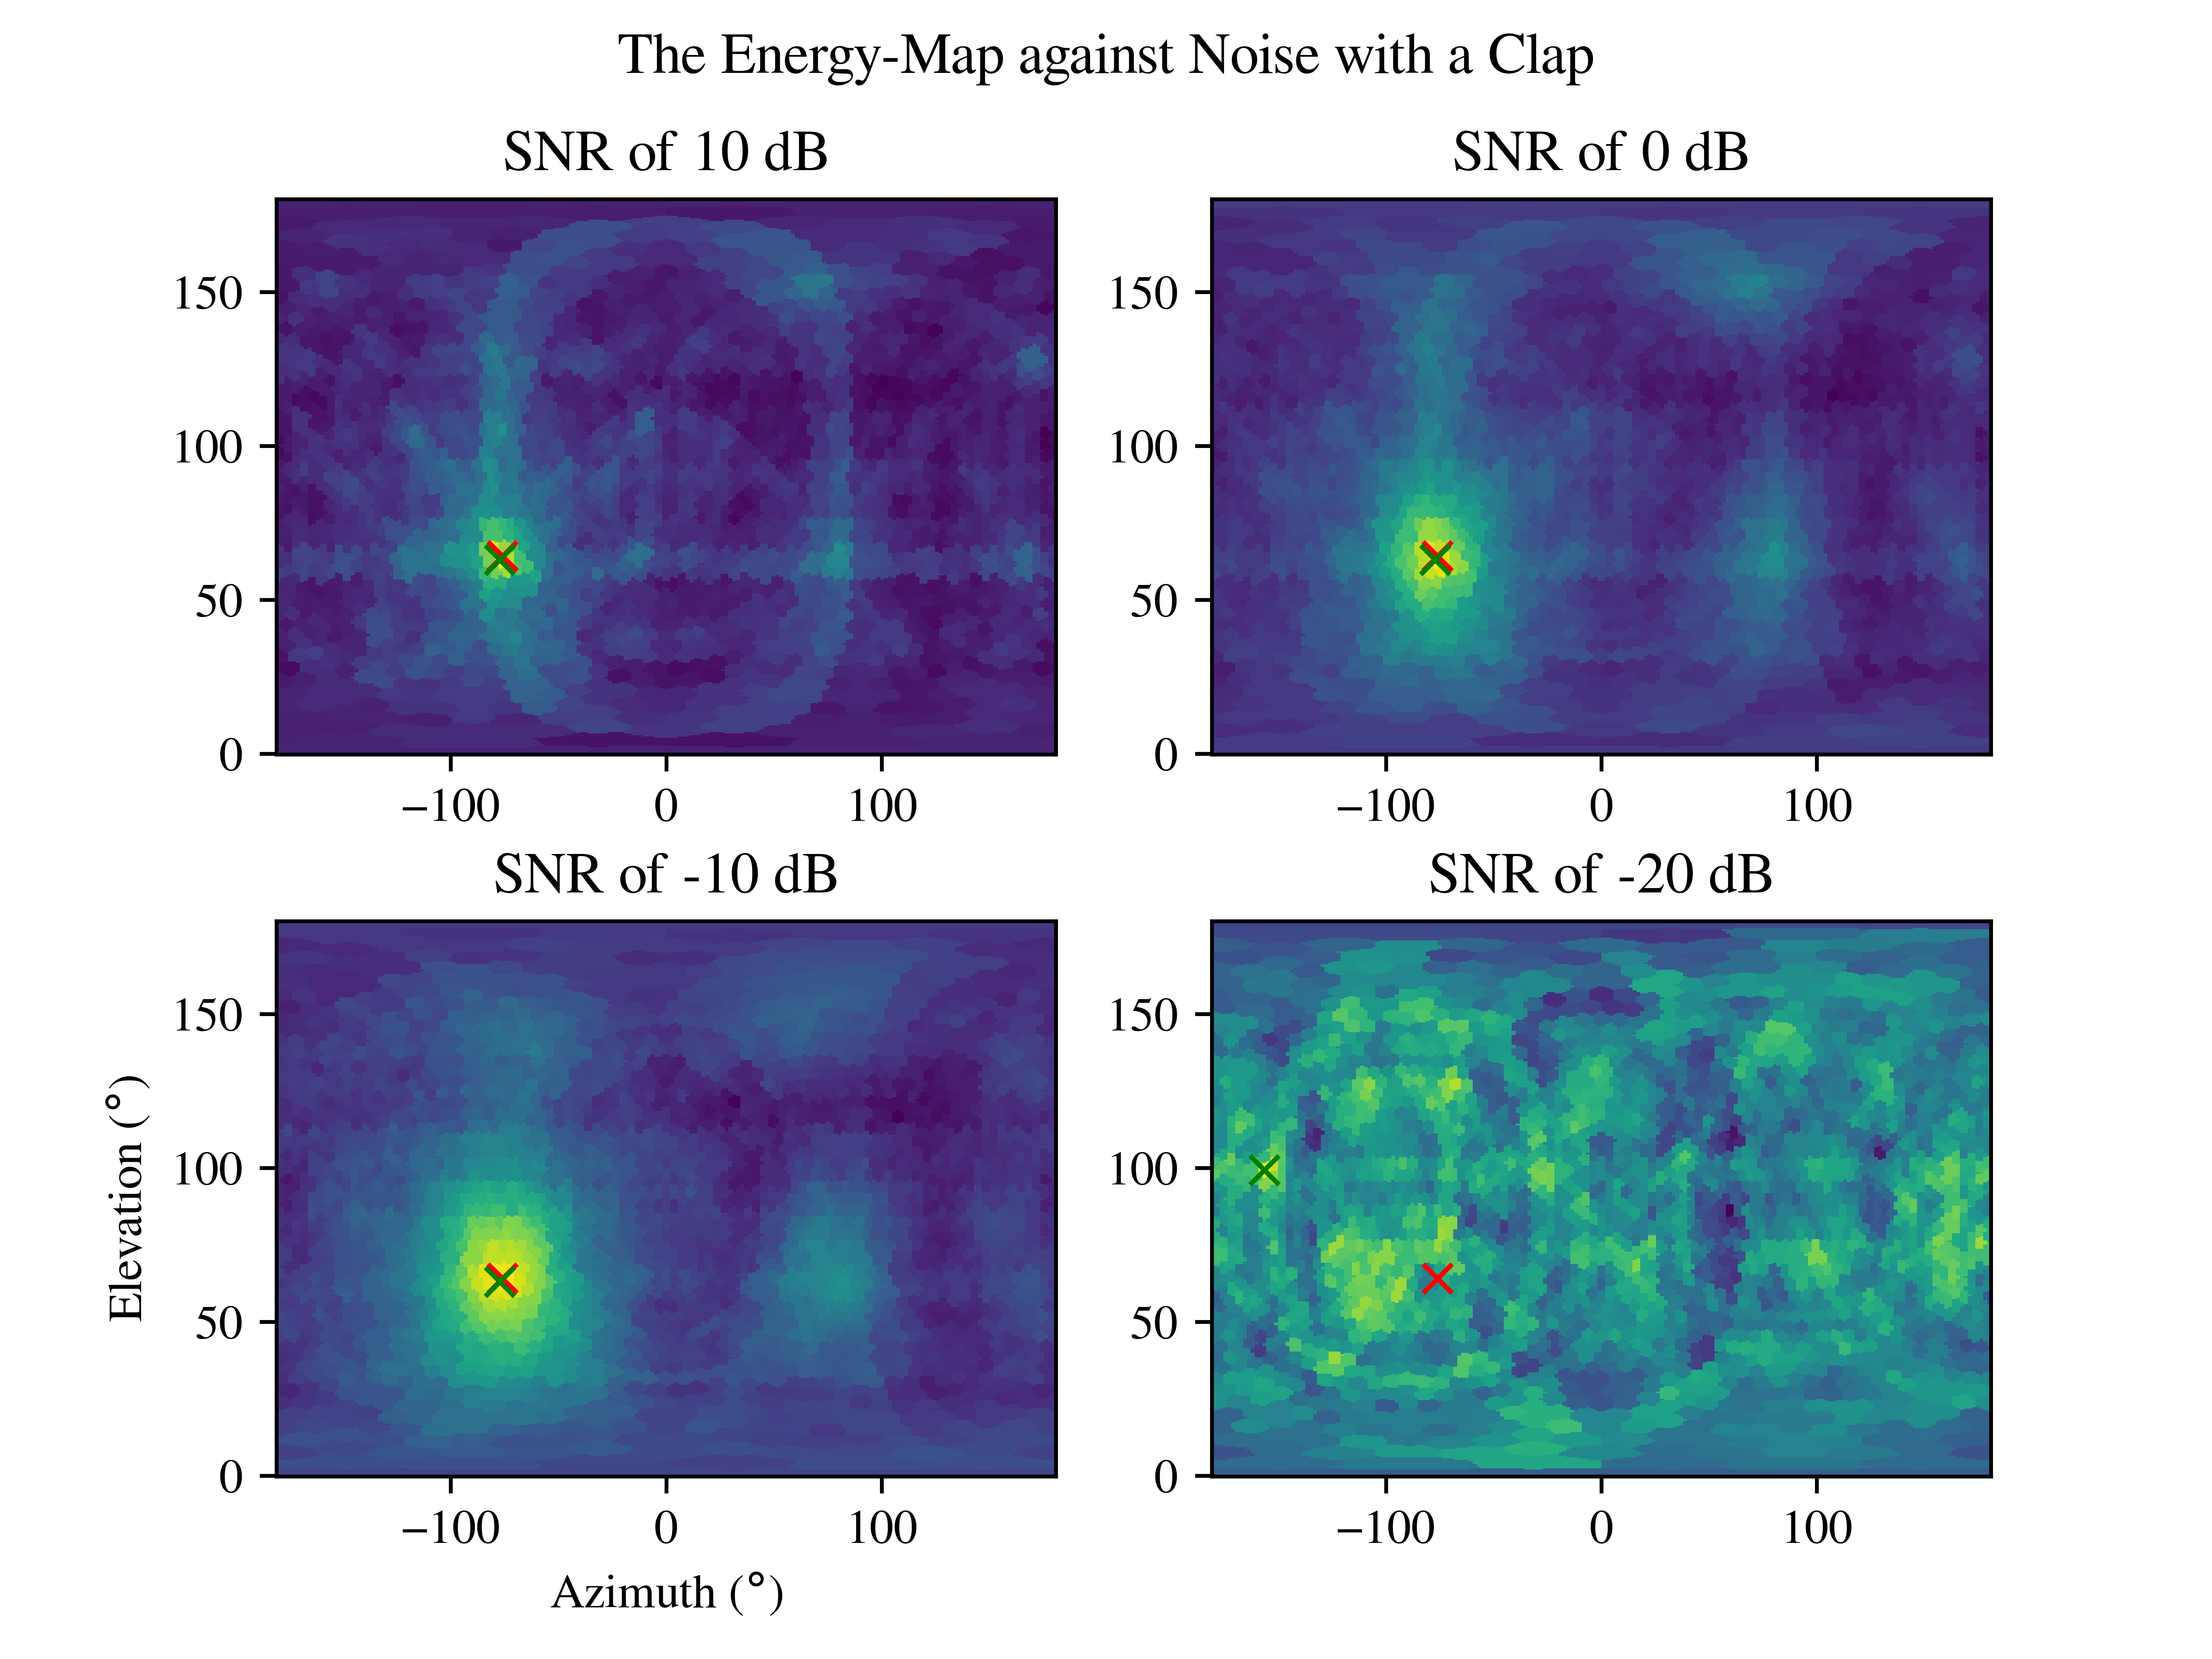
\includegraphics[width=0.9\textwidth]{../Python/main_method/noise/clap/map.png}
\centering
\caption{The energy-map of the SRP-PHAT beamformer was drawn with a clap as the source.}
\label{fig:mm_noise_map_clap}
\centering
\end{figure}

\begin{figure}[H]
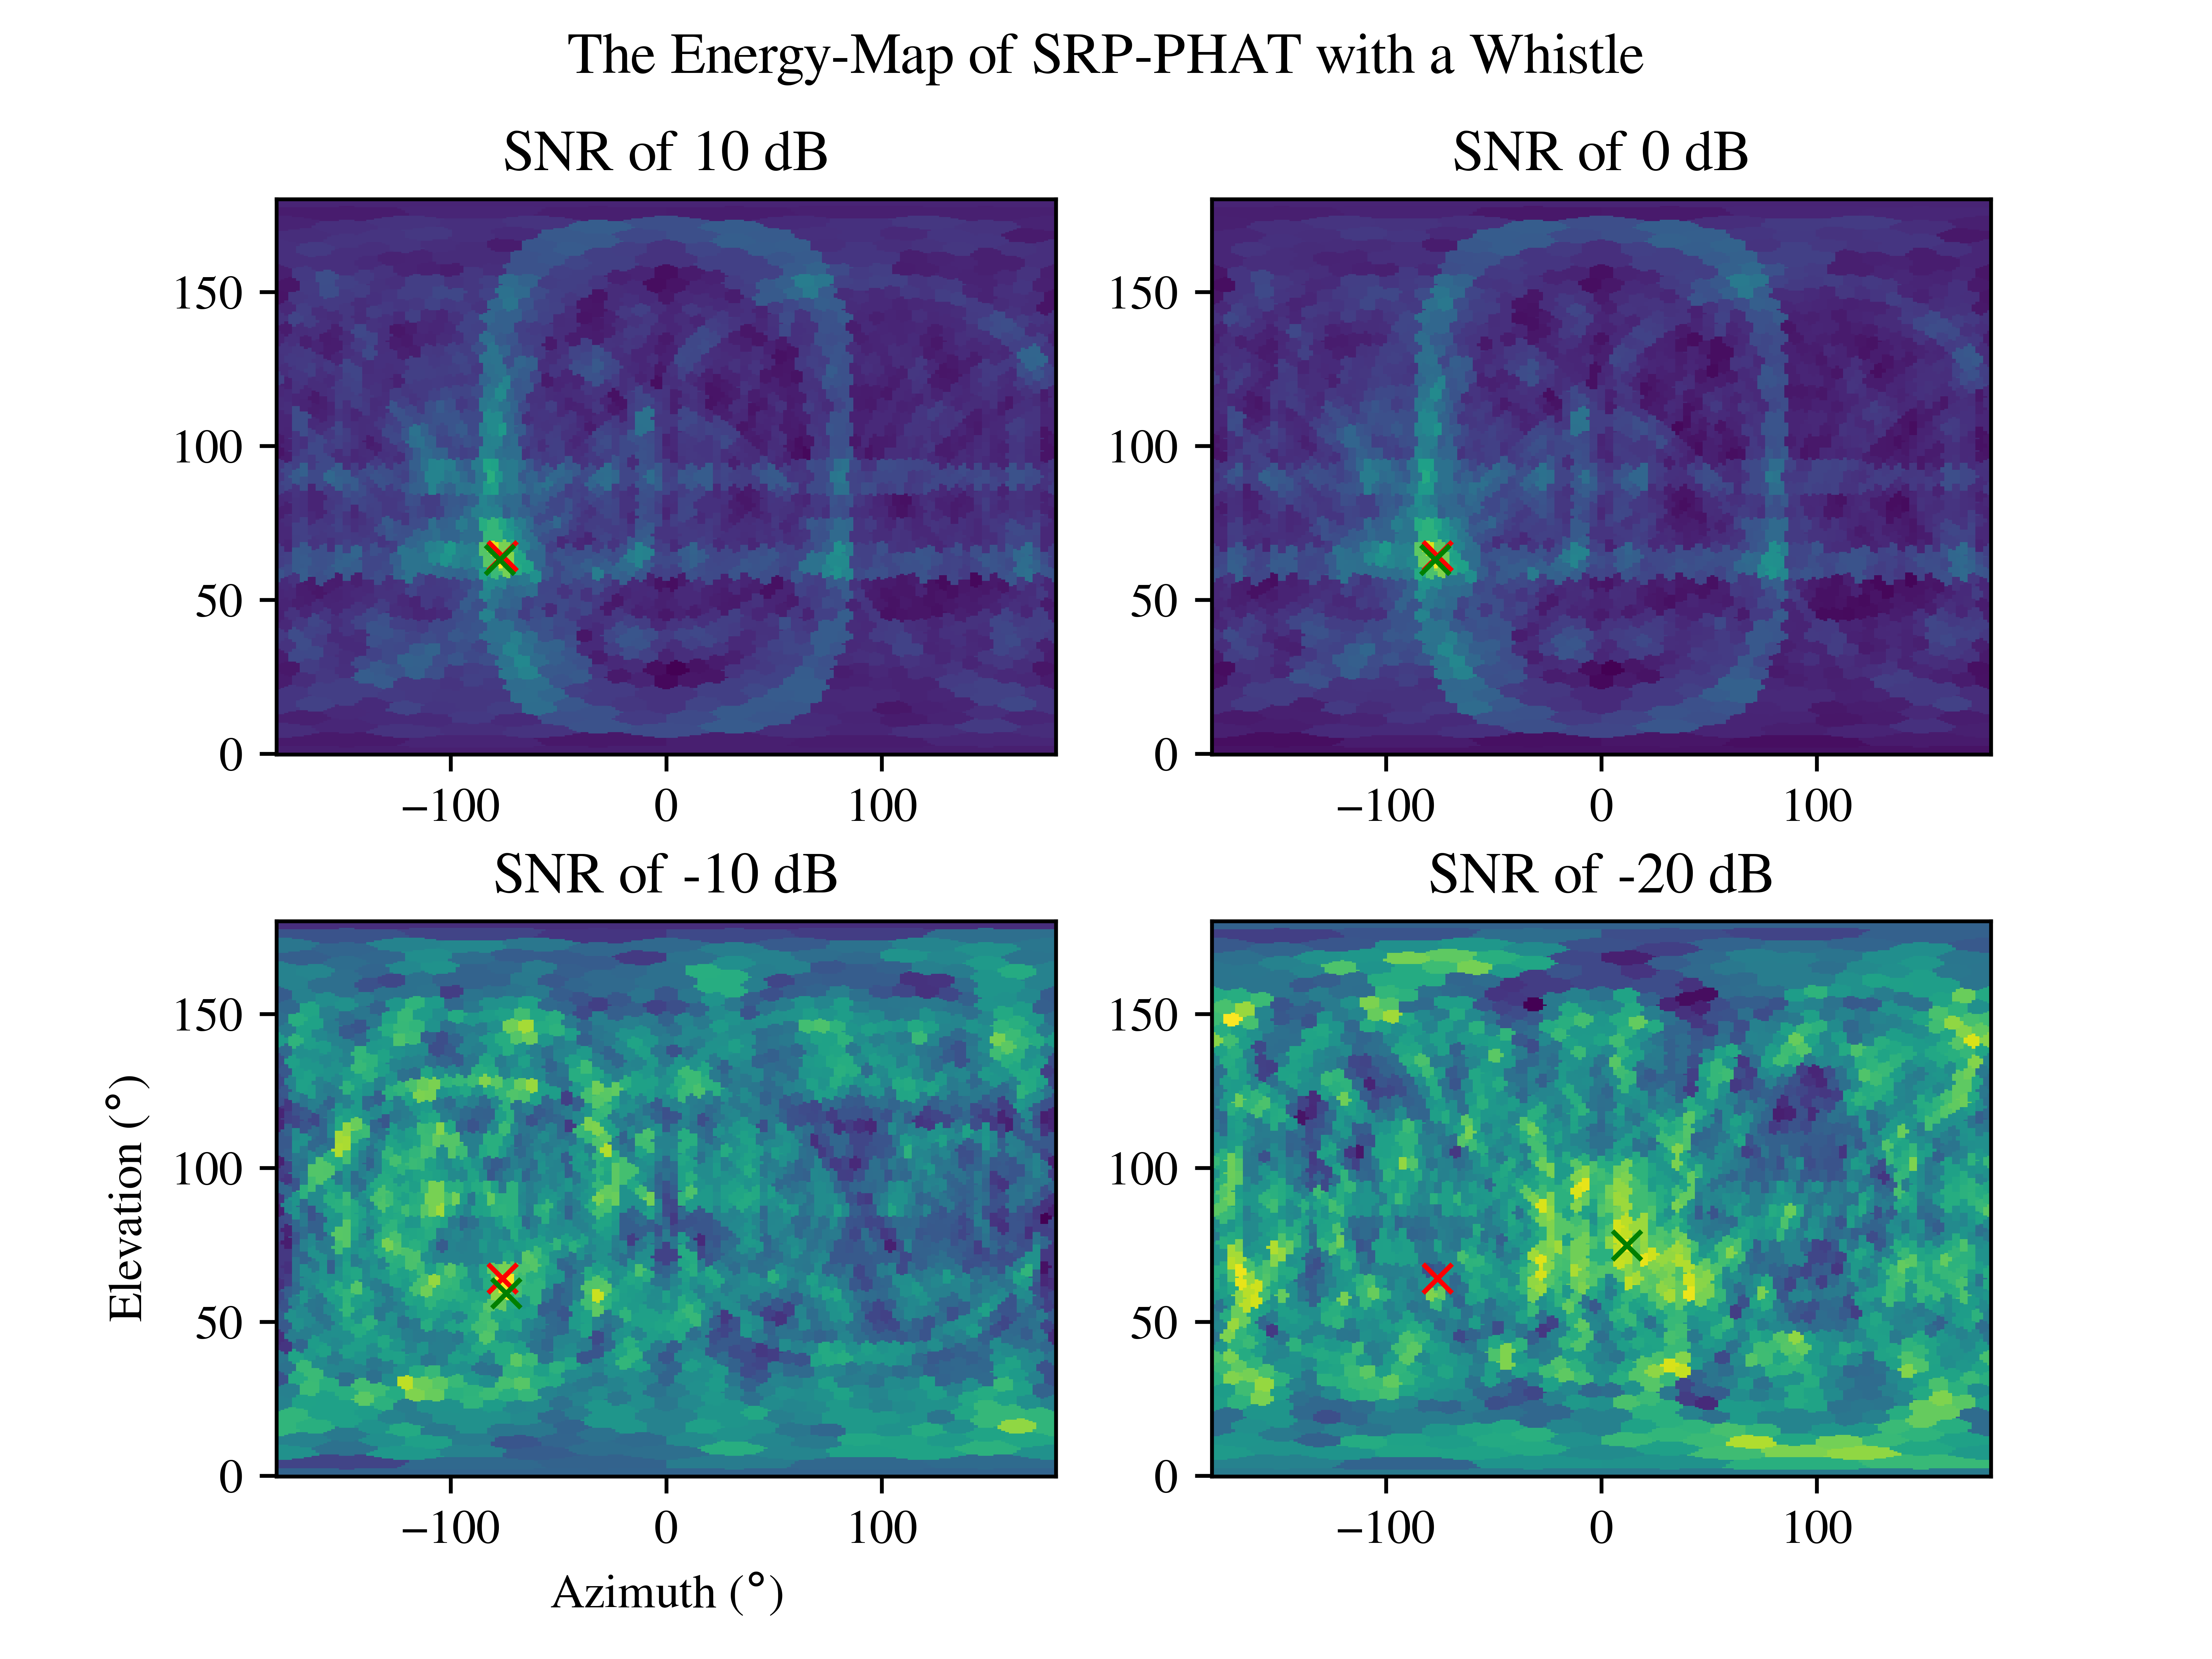
\includegraphics[width=0.9\textwidth]{../Python/main_method/noise/whistle/map.png}
\centering
\caption{The energy-map of the SRP-PHAT beamformer was drawn with a whistle as the source.}
\label{fig:mm_noise_map_whistle}
\centering
\end{figure}

\section{Performance against Distance}

The source was moved along a line at a -76.0 \si{\degree} azimuth at the same level with distances between 1 and 5 \si{m} away from the source.

As seen in Figure-\ref{fig:mm_distance_plots_clap}, both the accuracy and the precision worsened as the source was moved further away. This was expected since the SNR implicitly becomes worse when the source is further. However interestingly, both the mean and the variance worsened when the source was nearer than 3 \si{m}. This again was expected since the SRP algorithm relies on source being in the far field. As the source moves nearer, the approximations of the far field become less accurate.

\begin{figure}[H]
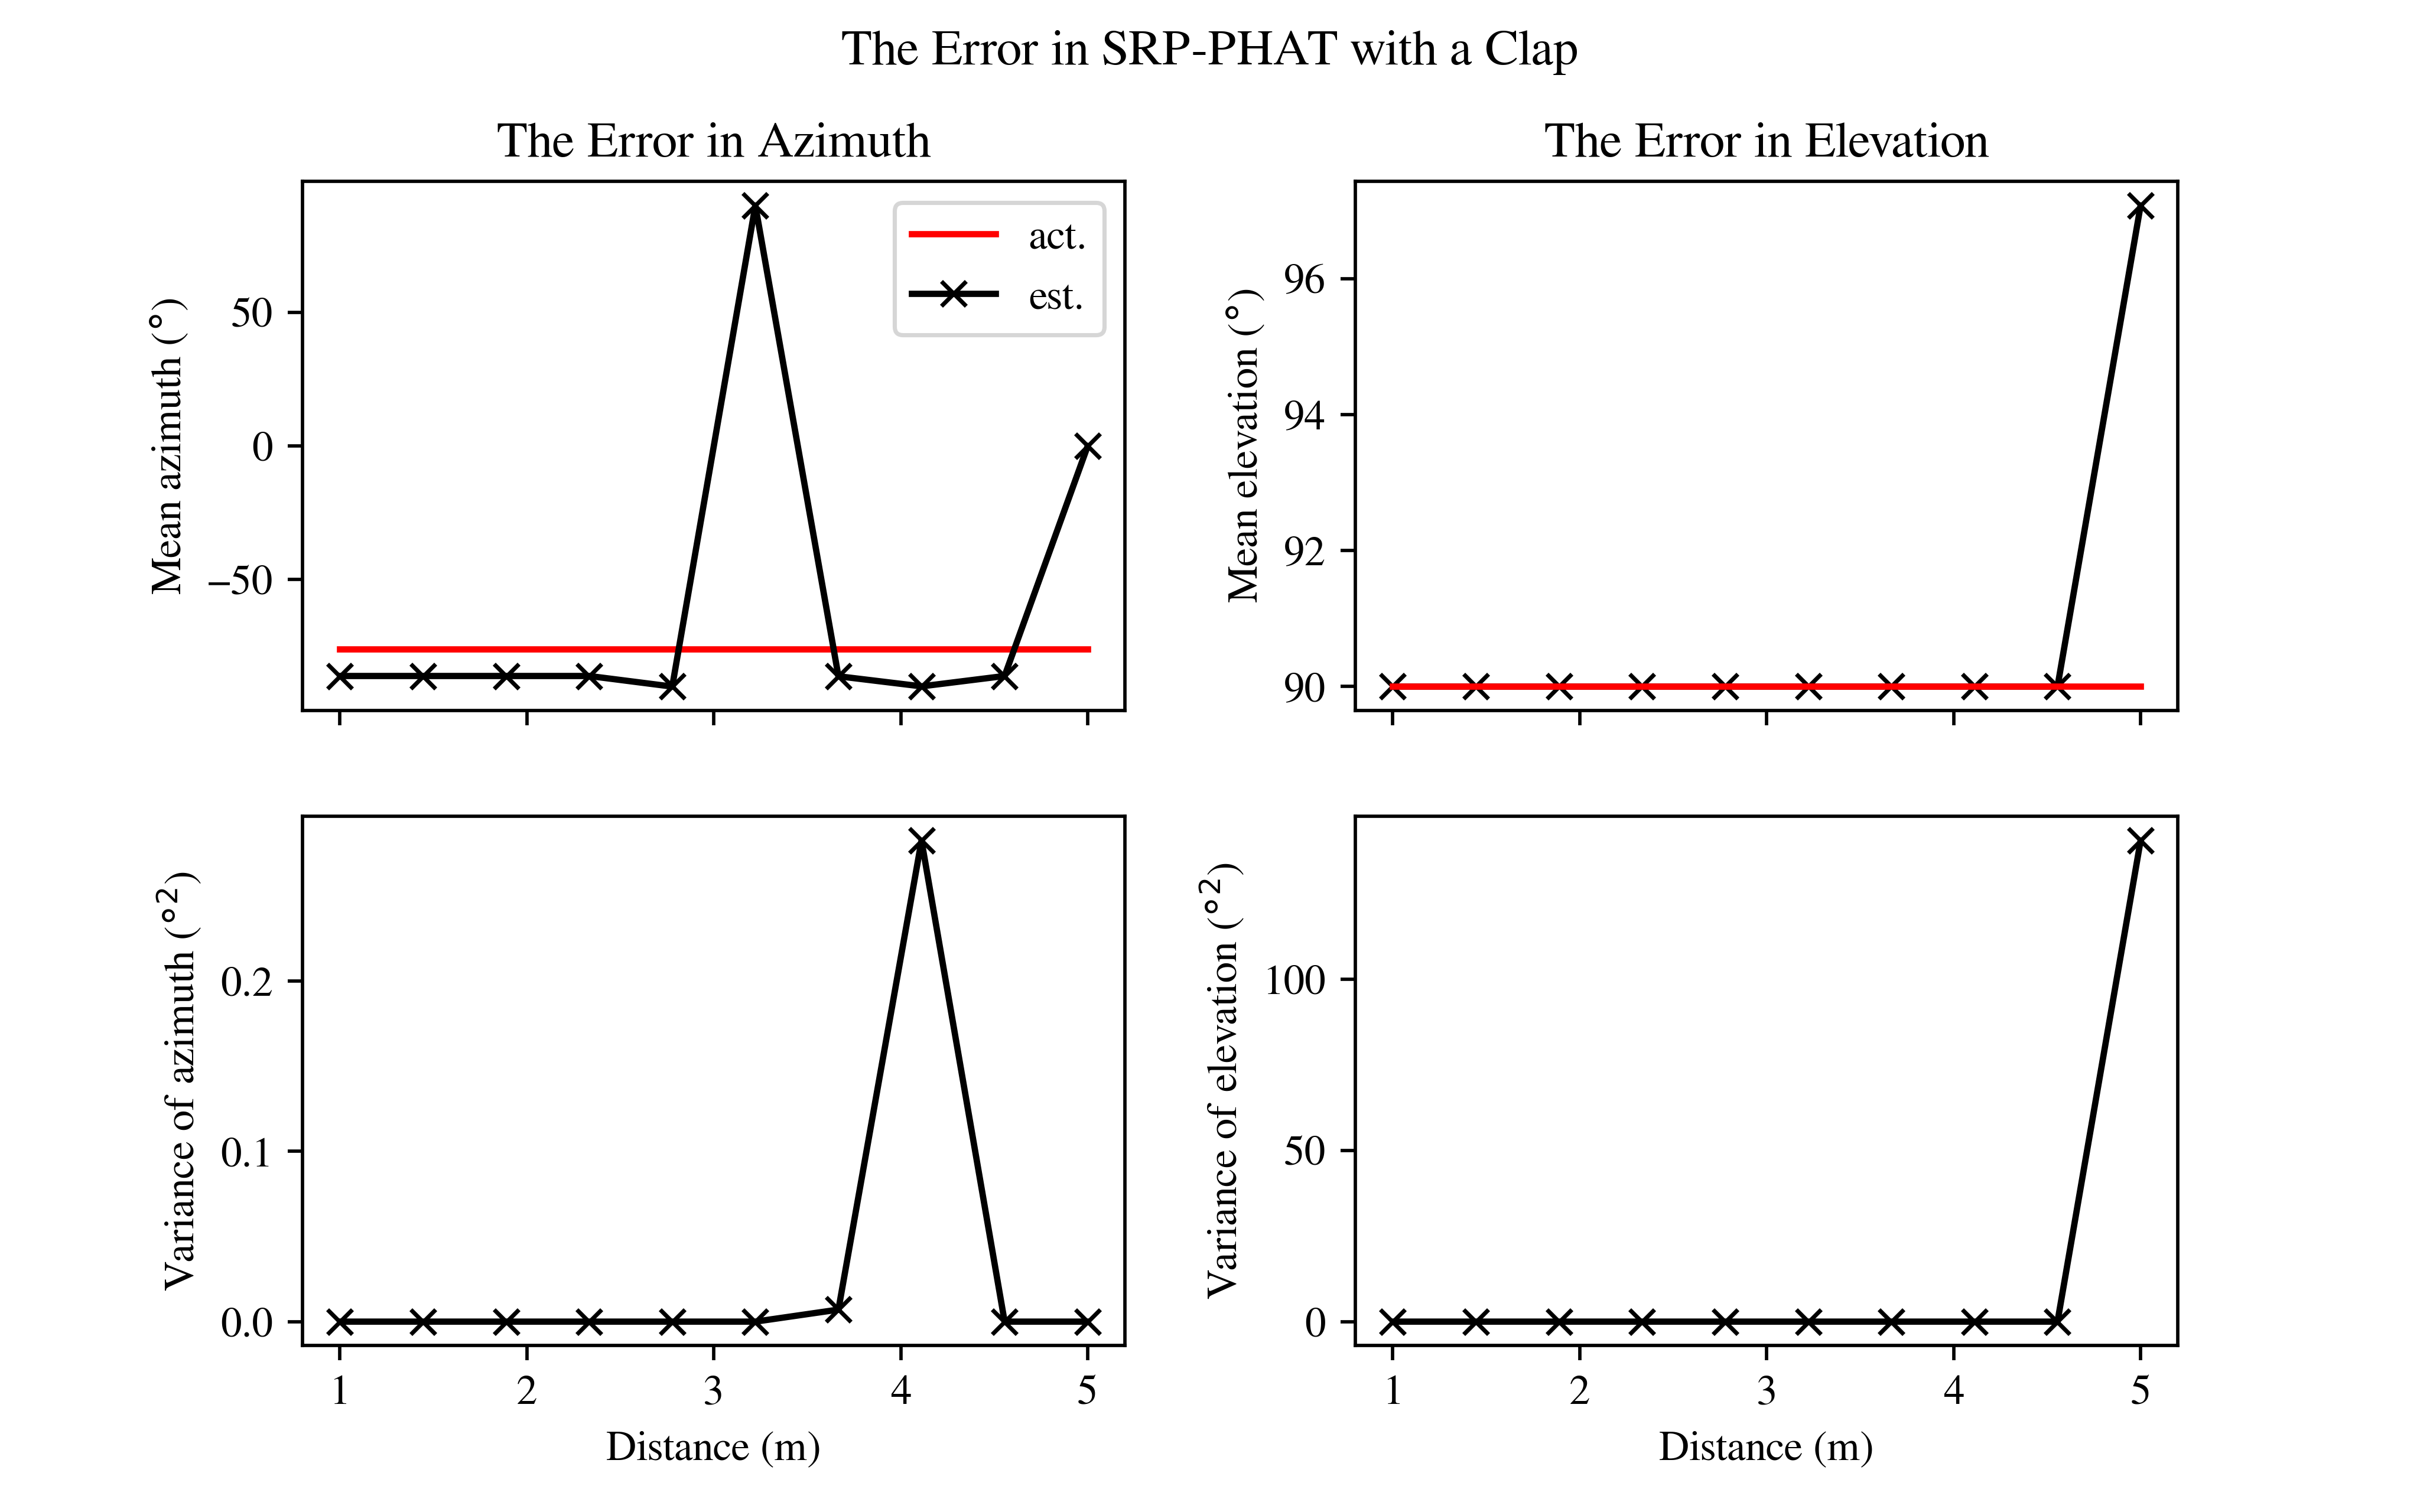
\includegraphics[width=0.9\textwidth]{../Python/main_method/distance/plots.png}
\centering
\caption{The statistical performance of the estimated direction was plotted against the distance with a clap as the source.}
\label{fig:mm_distance_plots_clap}
\centering
\end{figure}

\section{Effect of Delay} \label{Effect_of_Delay}

A big difference between this proposed design and many others in the literature was the fact that the array was to be embedded in the robot's head. Many of the examples in the literature were open arrays where all microphones nearly had perfect line of sight. With a closed array where there is a mostly solid object in between the microphones, a sound-wave would have to diffract around the head to reach some of the microphones. Given this and the fact that beamforming among other methods assume direct line of flight to calculate the TDOA, then this might affect the robustness of the system. This discrepancy shows itself up as a delay in the true time of flight.

Thus, a very simple rudimentary model shown in Figure-\ref{fig:delay_model} was made to emulate this effect. Given a spherical head and a microphone with no line of sight to the source, the delay could be computed by the angle between the microphone and the 'horizon' on the head's surface to which the source 'sees'; this horizon can be approximated as the line perpendicular to line between the source and the head's centre. This simple model could be taken as a rudimentary head-transfer-function.

\begin{figure}[H]
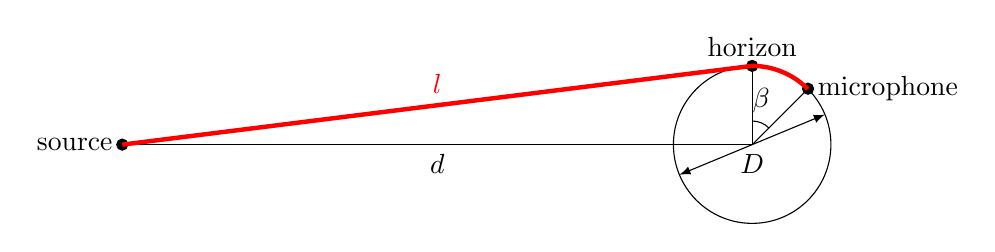
\begin{tikzpicture}
\draw (4,0) circle (1cm);
\draw[latex-latex, rotate around = {22.5:(4,0)}] (3,0) -- (5,0) node[midway, below,sloped]{$D$};
\draw (-4,0) -- node[below]{$d$} ++ (8,0);
\draw (4,0) -- (4.71,0.71);
\filldraw [black] (4.71,0.71) circle (2 pt) node[anchor=west]{microphone};
\draw (4,0) -- (4,1);
\filldraw [black] (4,1) circle (2 pt) node[anchor=south]{horizon};
\draw (4,0.3) arc (90:45:0.3) node[midway,above]{$\beta$};
\filldraw [black] (-4,0) circle (2 pt) node[anchor=east]{source};
\draw[ultra thick, red] (-4,0) -- (4,1) node[midway,above]{$l$};
\draw[ultra thick, red] (4,1) arc (90:45:1);
\end{tikzpicture}
\centering
\caption{The model for the delay given the spherical head where $D$ is the diameter, $d$ is the displacement between the source and the head's centre, $\beta$ is the angle between the horizon and the microphone, the red path is the sound-wave's path of flight, and $l$ is its length.}
\label{fig:delay_model}
\centering
\end{figure}

The longer path could be approximated as:
\begin{equation}
l = \frac{D}{2} \times \beta + \sqrt{d^2 + (D/2)^2}
\end{equation}
where $\beta$ is in radians.

The delay in sound would be the difference between the longer path $l$ and the original displacement $d$ between the microphone and the source as if there was direct line of sight.
\begin{equation}
\Delta t_{\text{delay}} = \frac{l-s}{c}
\end{equation}
where $c$ is the speed of sound, and
\begin{equation}
d = \lvert \vec{r}_m - \vec{r}_s \rvert
\end{equation}
where $\vec{r}_m$ is the coordinate of the microphone, and $\vec{r}_s$ is that of the source.

Of course, this crude model forsook true diffraction, where the frequency-response may not be uniform, and many other realities of sound such as reflections, etc. Yet, this model at least gave a lower bound of error because of the delay.

The source was set at $(6.5,3.5,2.5)$ where the SNR was varied from -20 to 25 \si{dB}. This setting would make it such that the azimuth was -45 \si{\degree} and that the elevation was 45 \si{\degree}. This was so that one microphone was the furtherst away from the source on the opposite side of the head and thus had the longest delay along the head. The three other microphones beside this one would also be slightly out of sight from the source. Thus, this setting would be the worst case.

As seen in Figure-\ref{fig:mm_delay_plots_clap}, both the accuracy and the precision were more dramatically affected around an SNR of 5 \si{dB}, against that in Figure-\ref{fig:mm_noise_plots_clap}. Of course, this was the worst and the most pessimistic setting. More lines of sight as discussed in the array's geometry might mitigate this.

\begin{figure}[H]
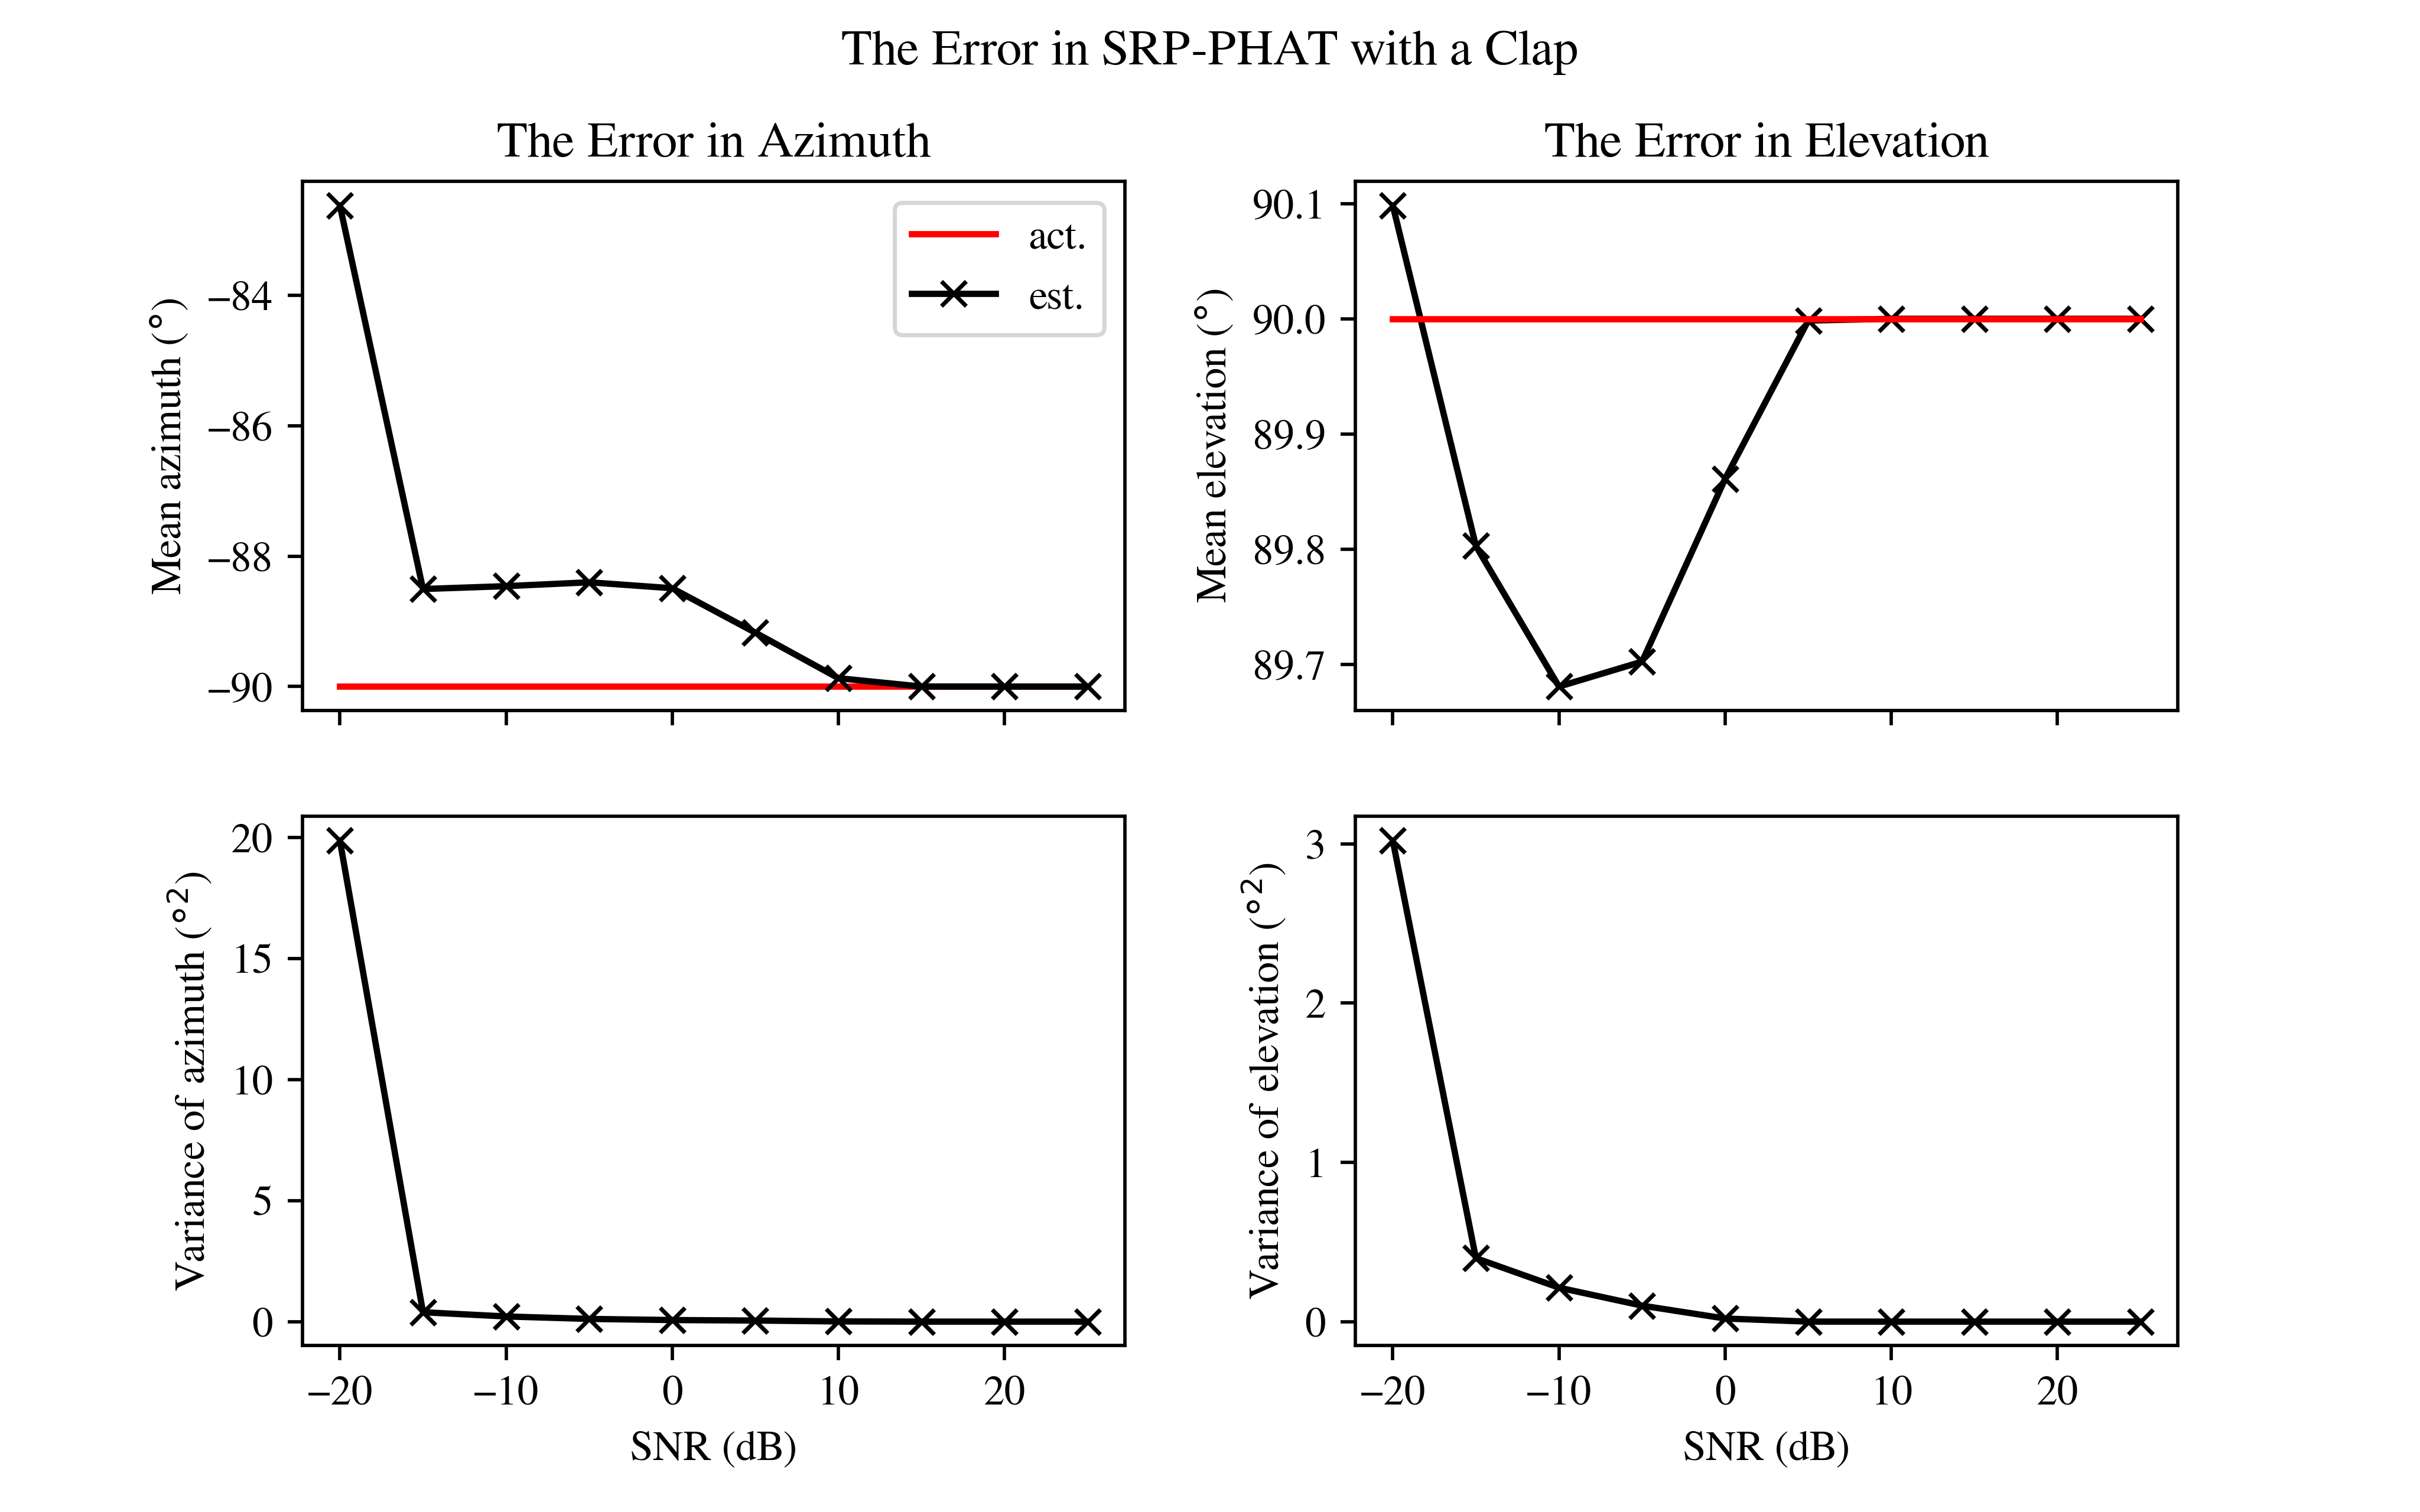
\includegraphics[width=0.9\textwidth]{../Python/main_method/delay/head/plots.png}
\centering
\caption{The statistical performance of the estimated direction was plotted against the noise with a clap as the source but with the emulated delay along the head.}
\label{fig:mm_delay_plots_clap}
\centering
\end{figure}

The maps in Figure-\ref{fig:mm_delay_map_clap} show an interesting sinusoid pattern that nevertheless breaks the beam down as the noise increases.

\begin{figure}[H]
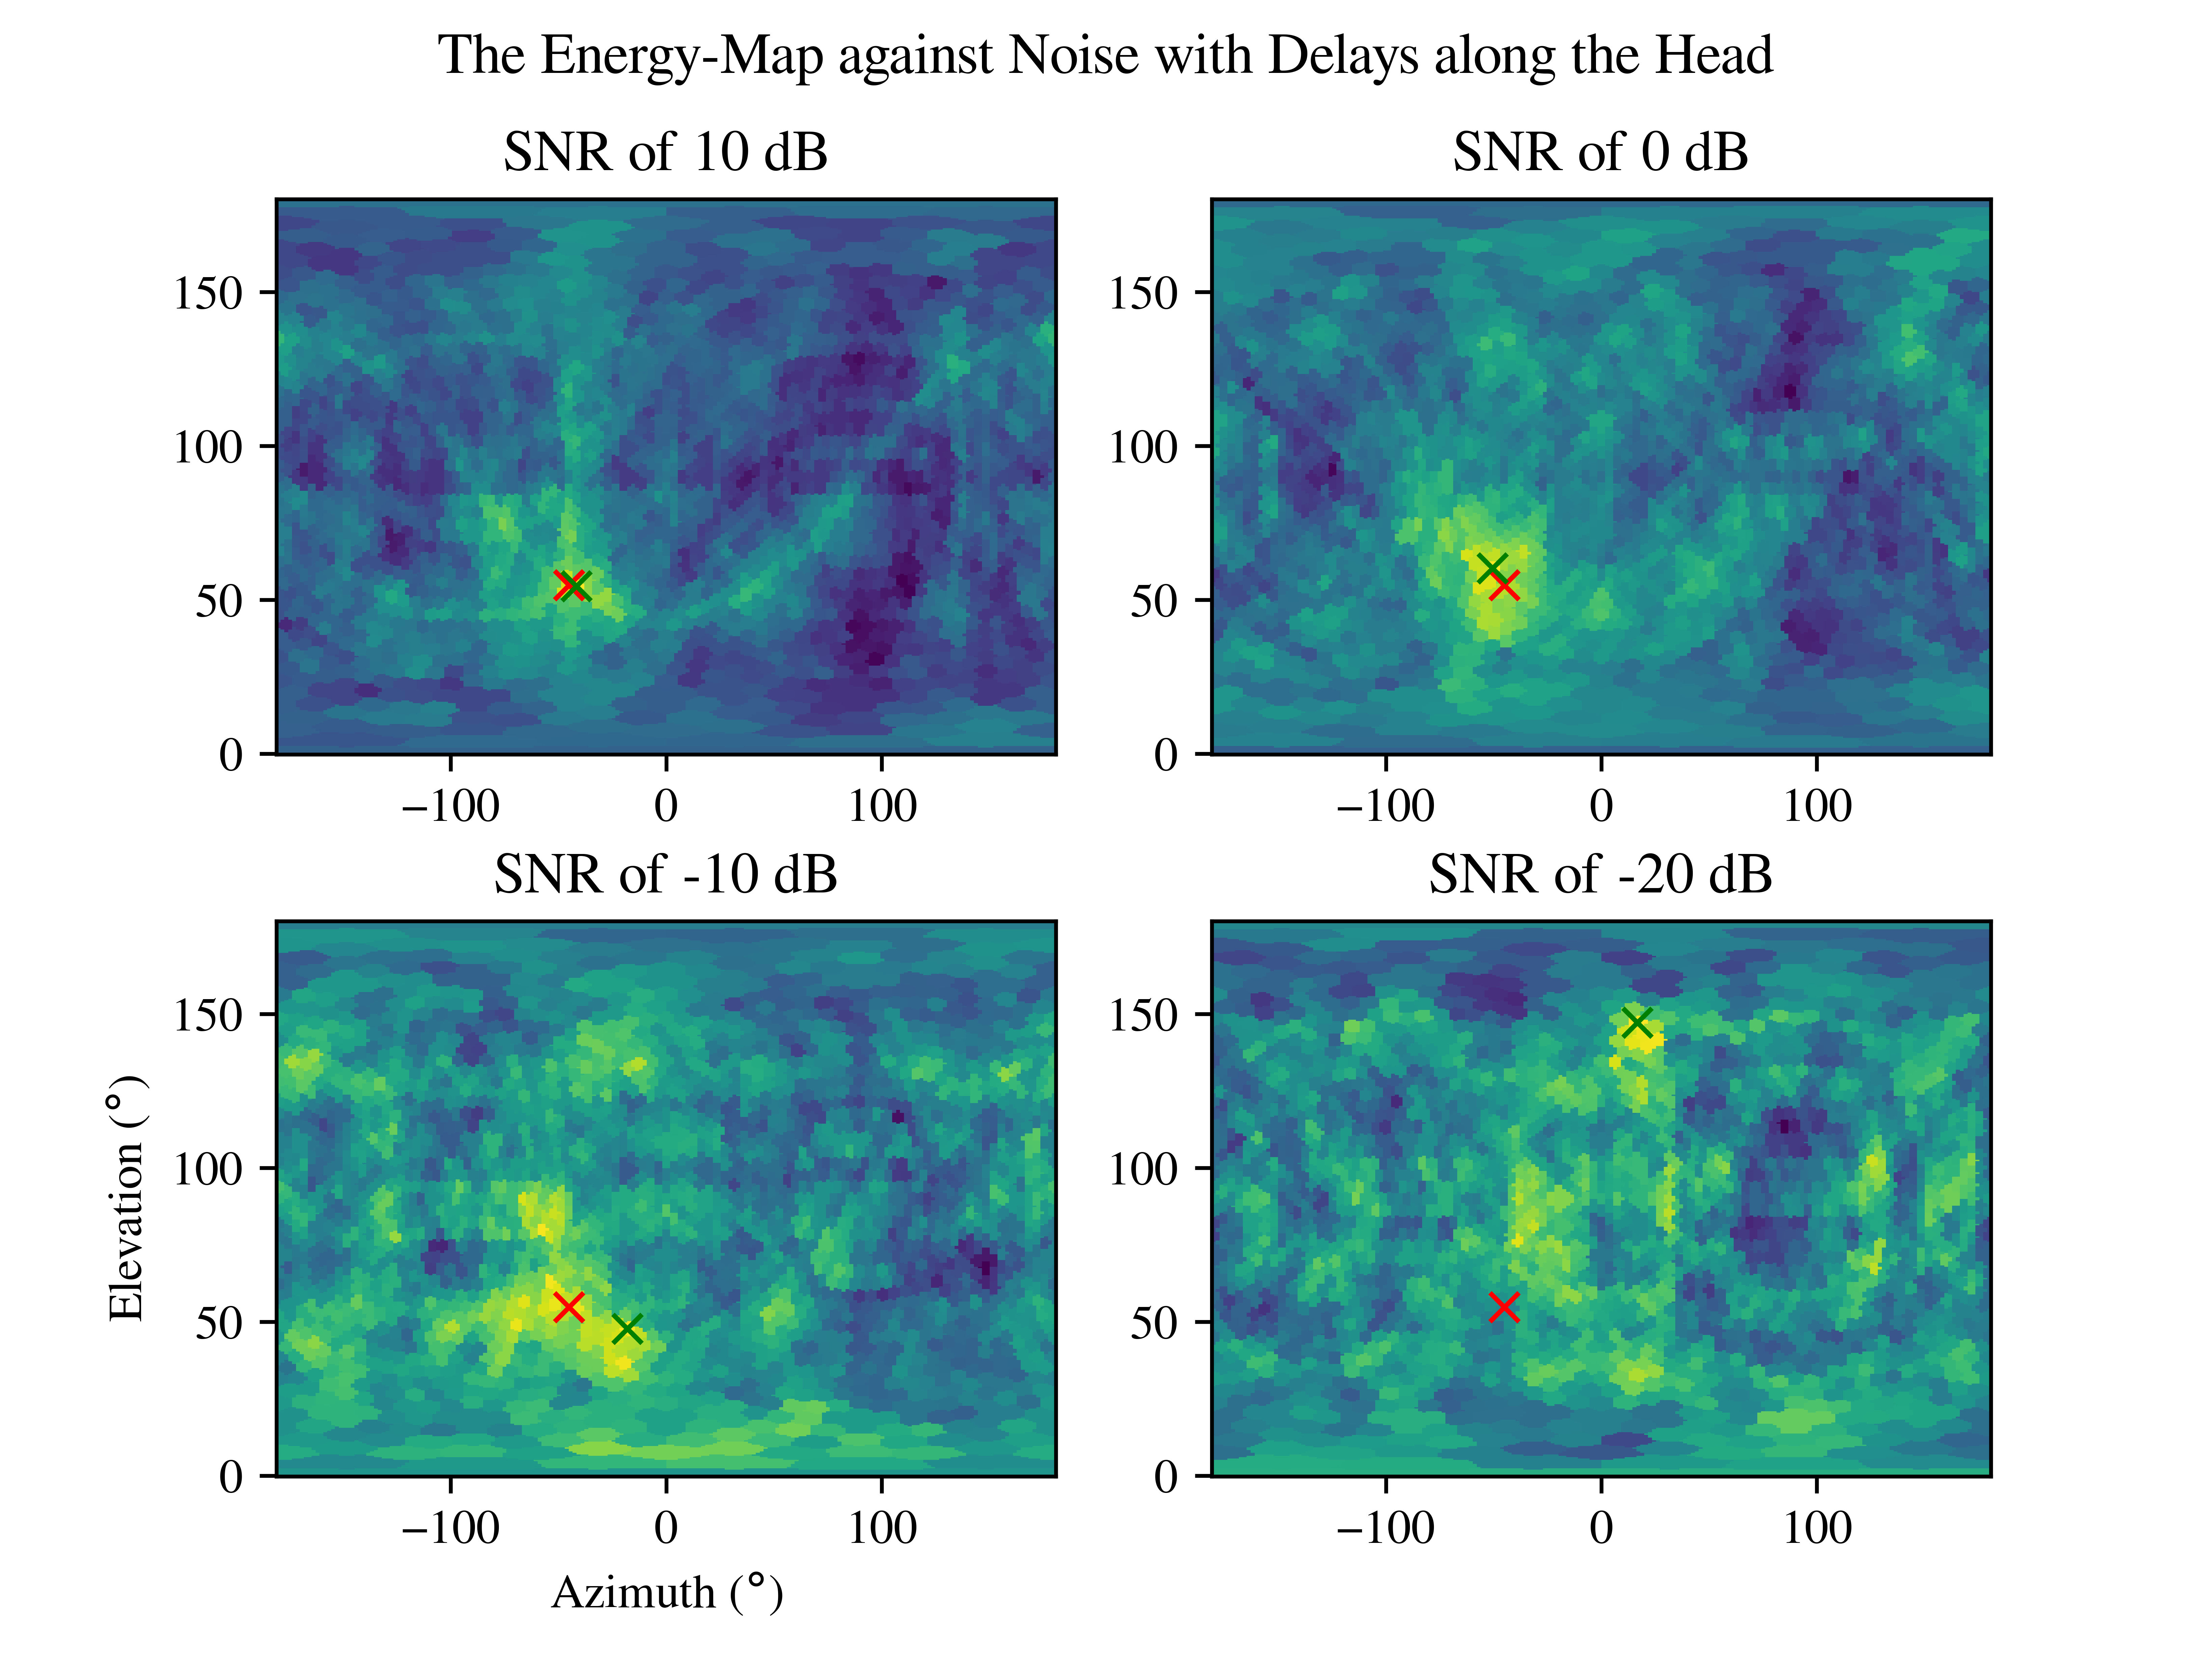
\includegraphics[width=0.9\textwidth]{../Python/main_method/delay/head/map.png}
\centering
\caption{The energy-map of the SRP-PHAT beamformer was drawn with a clap as the source and with the emulated delay along the head.}
\label{fig:mm_delay_map_clap}
\centering
\end{figure}

\section{Discussion}

It could be taken from these results that the proposed system would feasibly work with moderate levels of noise and even as low as a SNR of 0 \si{dB}. However, this is especially the case where the delay of the head was taken into mind which gives a more realistic prediction.

\chapter{Electronics Design}

A big part of this project was the electronics-design since many literature-examples do not attempt a small light-weight application. Therefore, this design was broken up into the research of microphones and audio in general, the chosen components, the chosen design, and then the printed circuit-boards (PCBs). Hereafter, this important chapter looks back over the design-process for the electronics. Note that the schematics are in the appendix.

\section{Overall Needs}

Since this system was to be used on a humanoid robot, an embedded solution was needed given that it would draw less power and be smaller and lighter. This made an added challenge given that most examples in the literature were implemented on either a SOC, a laptop, or even a desktop. Such an embedded solution would behave as a separate process that could handle the high throughput of data from the microphones and the high computation of the sound-source-localisation but then send simple results such as a direction through USB which would need relatively little throughput.

The biggest factor was the interface between the microphones and the main processor. There were a few potential kinds, namely:
\begin{itemize}
	\item analogue microphones through one or more analogue-to-dgitial-converters (ADCs),
	\item digital microphones through SPI, I\textsuperscript{2}S, etc.,
	\item and digital microphones through USB.
\end{itemize}
The last was deemed not appropiate since it would not be scalable to an embedded processor and might have needed more overhead in the firmware.

\section{Research of Microphones}

Before any major design was taken, the microphones and the audio-context more broadly first had to be taken into mind since the type of microphone could dictate the type of circuit, processor, etc. This section quickly touches on the background of the microphones.

The microphones and their respective interface needed:
\begin{itemize}
	\item to be sampled at 48 \si{kHz} at least,
	\item to be omnidirectional,
	\item to be sampled simultaneously exactly at the same time,
	\item to be reasonably robust to electrical interference,
	\item to not take up to much pre-processing to burden the processor's computation,
	\item to be able to handle at least eight microphones on one processor,
	\item to have a good SNR,
	\item and to have a good sensitivity.
\end{itemize}
The last two needed not to be too demanding but simply enough so that a wide range of sounds could be heard with enough clarity not to affect the phase.

\subsection{Sensitivity and Dynamic Range}

It is widely known that quiet rooms have a sound-pressure-level of 30 to 40 \si{dB_{SPL}}\cite{noauthor_comprehensive_nodate}, and converstions one metre away have that of 60 \si{dB_{SPL}}\si{dB_{SPL}}\cite{noauthor_decibel_nodate}. Louder environments such as those with machinary and tools tend to have a level of around 90 \si{dB_{SPL}}\cite{abbott_decibels_nodate}. Very loud sounds like a chainsaw about one metre away, aeroplanes, etc. have a level of 120\si{dB_{SPL}}\cite{noauthor_decibel_nodate}. 

Anything above that is passed the threshold of pain\cite{noauthor_decibel_nodate}. Although it was not expected that the system must have localised sounds of every possible level, it would be best if the system could localise within a range as deep as possible.

However, most microphones would have a noise-floor which is often somewhere between 20 and 40 \si{dB_{SPL}} and is often written as a SNR relative to a single tone of 94 \si{dB_{SPL}} at 1 \si{kHz}\cite{sennequier_pre-amplifying_2015}. This floor bounds how quiet the sounds can be heard.

Furthermore, the sensitivity affects the dynamic range of levels. This is given as the ratio between the output often in volts and the pressure in Pascals\cite{lewis_understanding_nodate}, but it is most often written in decibels and in most datasheets for a single tone of 94 \si{dB_{SPL}} at 1 \si{kHz}, e.g. in \cite{noauthor_spw2430hr5h-b_2014}. The higher the sensitivitiy is, the higher the voltage is. Most electret and MEMS microphones have a sensitivity between -46 and -35 \si{dBV}. More importantly, the higher the sensitivity is, the less gain is needed which can add thermal noise to the signal \cite{simmons_microphones_2021}.

Other specifications of microphones are the total harmonic distortion (THD), and the maximum acoustic input. Most common electret and MEMS microphones have a THD less than 1 \% at an acoustic input of 94 \si{dB_{SPL}} and a higher THD of around 10 \% at a maximum acoustic input of around 120 \si{dB_{SPL}}. However, harmonic distortion might not be a big problem since it does not affect the spectral phase, only the spectral magnitude.

\subsection{Interface}

Small microphones in electronics use many different kinds of communication. The main kinds are:
\begin{itemize}
	\item analogue through an ADC,
	\item pulse-density-modultion (PDM),
	\item I\textsuperscript{2}S, 
	\item SPI,
	\item I\textsuperscript{2}C
\end{itemize}

The first three are the most common, and the last two share similarities with I\textsuperscript{2}S.

\subsubsection{Analogue through an ADC}

The most basic MEMS microphone is one that has its own pre-amplifier and outputs a small yet measurable voltage\cite{lewis_analog_nodate}. This output is often weak and has a higher impedance. So, another amplifier circuit may be needed before an ADC. Indeed, an analogue anti-aliasing filter is also needed which may add complexity to the electronic design.

Most processors on the market, i.e. microcontrollers, DSPs, etc., have two or three ADCs but with multiplexed channels. However, for each ADC, the channels are sampled sequentially by a single sample-and-hold after the multiplexer. Thus, this means that the channels can never truly be sampled simultaneously. Therefore, an external ADC chip that could sample simultaneously must have been chosen. Such chips can often communicate through either a serial or a parallel interface, e.g. SPI. Given that enough samples from each microphone can be output on the interface within a sample-period, then a digital interface should not affect the timing.

Otherwise, the simultaneous sampling could have been forsaken so that system sampled sequentially instead, and the design was simpler, but it was unpredictable how this imprecise sampling would have affected the algorithm. It was therefore safer to assume the worst and design the system to sample simultaneously.

\subsubsection{PDM}

PDM microphones have additional circuitry made up of an ADC and modulator\cite{lewis_analog_nodate}. Pulse-density-modulation (PDM) is where the sound-signal is encoded as bits whose density correlates to the sound's amplitude. These bits are output by a given clock-signal. Thus, PDM microphones can be connected to SPI, I\textsuperscript{2}S, and other interfaces on a microcontroller. For example, some STM32s have modules specifically for communicating with PDM microphones that can allow up to eight microphones\cite{noauthor_interfacing_2019}. At worst, the delay between two channels can be half the clock-cycle which is often in the range of \si{MHz} and thus not too long\cite{lewis_analog_nodate}.

This stream of bits is then filtered, decimated, and converted to a PCM signal of integer values. However, because of this, there may be more computational burden since it has to be done by the processor.

\subsubsection{I\textsuperscript{2}S and Other Serial Interfaces}

Like SPI and I\textsuperscript{2}C, I\textsuperscript{2}S allows a microphone to output a word representing a value on a serial data-line along with a clock-signal\cite{lewis_analog_nodate}. Thus, the data can be output at a much lower rate. Some microcontrollers allow three or four I\textsuperscript{2}S interfaces, e.g. the STM32H723 \cite{noauthor_arm_2021}, each can allow two microphones. Therefore, some microcontrollers can allow eight microphones in theory. However, there seems to be no formal guarantee that the samples of each microphone are simultaneous or even near such.

\subsection{Anti-aliasing Filter}

If an analogue output were to be read by an ADC from the microphone, then an analgoue anti-aliasing filter must have been used lest noise and other components of higher frequency in the stop-band were folded back into the pass-band\cite{horowitz_1351_2015} \cite{noauthor_filter_2002}.

The filter's phase-response should be carefully taken into mind. Although a perfect linear phase-response was not needed, the phase-response would have to be consistent between channels, i.e. microphones, since the GCC-PHAT only takes the relative difference in phase between two such channels. Therefore, components like capacitors would have to be precise enough to not propogate any variance in the phase-response. On the other hand, the magnitude-response was not too important since GCC-PHAT will whiten the spectrum anyway.

Furthermore, most analogue filters cannot have both a steep roll-off and a good phase-response. Even then, filters of higher order have more components and complexity and can thus lead to inconsistencies between the channels.

One method is to sample much higher than the -3 \si{dB} cut-off frequency such that the gain is around -20 or -40 \si{dB} at the Nyquist frequency\cite{horowitz_1351_2015}. Thus, higher frequencies past this point are attenuated much more than the -3 \si{dB} bandwidth and do not affect the passband when they are folded back. Furthermore, after the signal has been sampled, a digital filter can decimate the signal such that its Nyquist frequency is the -3 \si{dB} frequency of the analogue filter before. Such a digital filter may need a high order, or number of taps. This whole process is often known as \textit{oversampling}.

\section{Chosen Components}

Before the circuit was designed, appropriate components had to chosen so that overall design could be made. The process began first at the beginning of the signal-path, i.e. the microphone, and then followed its way to the end, i.e. the processor. Thus, this section talks about each major component.

\subsection{Microphone}

Many microphones were considered, but one that stood out was the SPH1642HT5H-1 since it has a relatively high sensitivity of -38 \si{dBV} which means that it needs less gain \cite{noauthor_sph1642ht5h-1_2017}. It also is a MEMS-on-lid design and thus has a wide bandwidth \cite{noauthor_sisonic_nodate}.

\subsection{Preamplifier}

Each microphone's signal needed to be pre-amplified before the transmission-cable to the motherboard where the ADC and processor was. Furthermore, given nearby WiFi antennae, servo-motors, and switching converters on the robot itself, the signal must have been differential and sent over a twisted pair.

Therefore, the TS472 audio amplifier chip was chosen since it has a differential output, a constant bandwidth of 40\si{kHz} despite the gain, and a low noise of 10 \si{nV/sqrt{Hz}} \cite{noauthor_very_2009}. It is also built specifically for this application with microphones and for which gives its own bias-voltage lest a separate 3.3 \si{V} rail is needed.

This analogue circuitry must have been as close to the microphone as possible to ready the signal for the twisted pair; therefore, each microphone would have its own daughterboard with this pre-amplifier.

\subsection{Difference-Amplifier}

To receive the differential signal across the twisted pair from the daughterboard, a difference-amplifier was needed to convert it to a single-ended signal and drive it for the ADC's inputs. A difference-amplifier can be simply made from an op-amp and four resistors \cite{horowitz_514_2015}. The resistors would not have the exact same resistances because of their tolerances. Although the CMRR of the amplifier may be less given the slightly mismatched resistors, it was not a problem in this application since the common-mode voltage from the microphone's preamplifier was unlikely to be high.

Thereby, a TLV272 was chosen since it has two op-amps in one package, has a rail-to-rail output which stops harmonic distortion for loud signals, and has a good GBWP of 2 \si{MHz} and a high slew-rate of 2 \si{V/\micro s} \cite{noauthor_tlv27x_2016}. Even with a gain of 10, the total bandwidth would be 200 \si{kHz} which would still be high enough.

\subsection{External ADC Chip}

An external ADC chip was needed that:
\begin{itemize}
	\item can sample at 480 \si{kHz},
	\item can communicate eight samples within one sample-period,
	\item can sample eight channels simultaneously,
	\item and has a reasonably compatible digital interface whether it is serial or parallel.
\end{itemize}

Few ADC chips could sample simultaneously. As such, the AD7606B was chosen since it was one of the few that could. It had eight channels and could sample up to 800 \si{kHz} and communicate through either a serial interface or a parallel interface. 

It also had its own anti-aliasing filters for each channel. The cut-off frequency of which varied between 9 and 22.5 \si{kHz} depending on the selected voltage-range. These frequencies are nevertheless enough for audio. Given the resolution of sixteen bits, the SINAD was about 87.7 \si{dB} for a range of $\pm5\si{V}$.

Furthermore, the AD7606B has pseudo-differential true bipolar inputs; this means that each channel has a ground-pin and can receive a twisted pair as an input. However, this was not needed since a separate difference amplifier was used.

Also, the chip came as a QFP which is realtively easy to solder by hand. Many other ADCs came in QFN which has pads underneath the chip.

\subsection{Processor}

The processor could be either a simple micrcontroller or a digital signal processor (DSP); the latter might be more suited to this application. Although most micrcontrollers and DSPs have their own ADC, most if not all do not have simultaneous sampling. Therefore, a processor is needed that:
\begin{itemize}
	\item can communicate with either an external ADC or communicate with digital microphones,
	\item has a reasonably high clock-speed,
	\item has hardware-accelerated FFT among other mathematical optimisations,
	\item and can communicate through USB or any other simple interface e.g. UART to send results.
\end{itemize}

A STM32H723VG was chosen largely since it has an Arm Cortex-7 CPU \cite{noauthor_arm_2021}. This means that it can do hardware-accelerated FFT \cite{noauthor_digital_2018}. The H7 processors in particular are some of the fastest STM32 microncontrollers. The STM32H723VG in particular was chosen since it could have up to four I\textsuperscript{2}S interfaces which could be used with digital microphones as a back-up to analogue microphones.

Another processor that was considered was the TMS320C5515 which is a DSP with a slightly better hardware-accelerated FFT \cite{noauthor_tms320c5515_2013} \cite{mckeown_fft_2013}. But it only came in BGA package which is hard to solder by hand. Also, STM32s were an already well known family of microcontrollers to develop therewith.

\subsection{Other Components}

Other such components and interfaces were:
\begin{itemize}
	\item a L78M05 5 \si{V} linear regulator to step down from 12 \si{V} for the analogue circuitry \cite{noauthor_precision_2020},
	\item an UA78M33 3.3 \si{V} linear regulator to step down from 5 \si{V} for the digital circuitry, i.e. the STM32 and the ADC's digital interface \cite{noauthor_a78mxx_2015},
	\item and a USB micro-B socket connected to the STM32's internal full-speed physical layer.
\end{itemize}

\section{Chosen Design}

Here, this section talks about the decisions made during the design, mostly the signal-path from the microphones to the processor. For the full design, see Appendix-\ref{Schematics_of_Electronics}.

\subsection{Overall Design}

The chosen electronics-design was to have each microphone and its preamplifier on separate daughterboards and the STM32 processor and the external ADC on one motherboard. As seen in Figure-\ref{fig:design_overall}, the microphone's signal is first preamplified before being send down a twisted pair as a differential signal and then received by a difference-amplifier which converts it back to a single-ended signal for the ADC. Finally, there is also a USB connection to output results.

\begin{figure}[H]
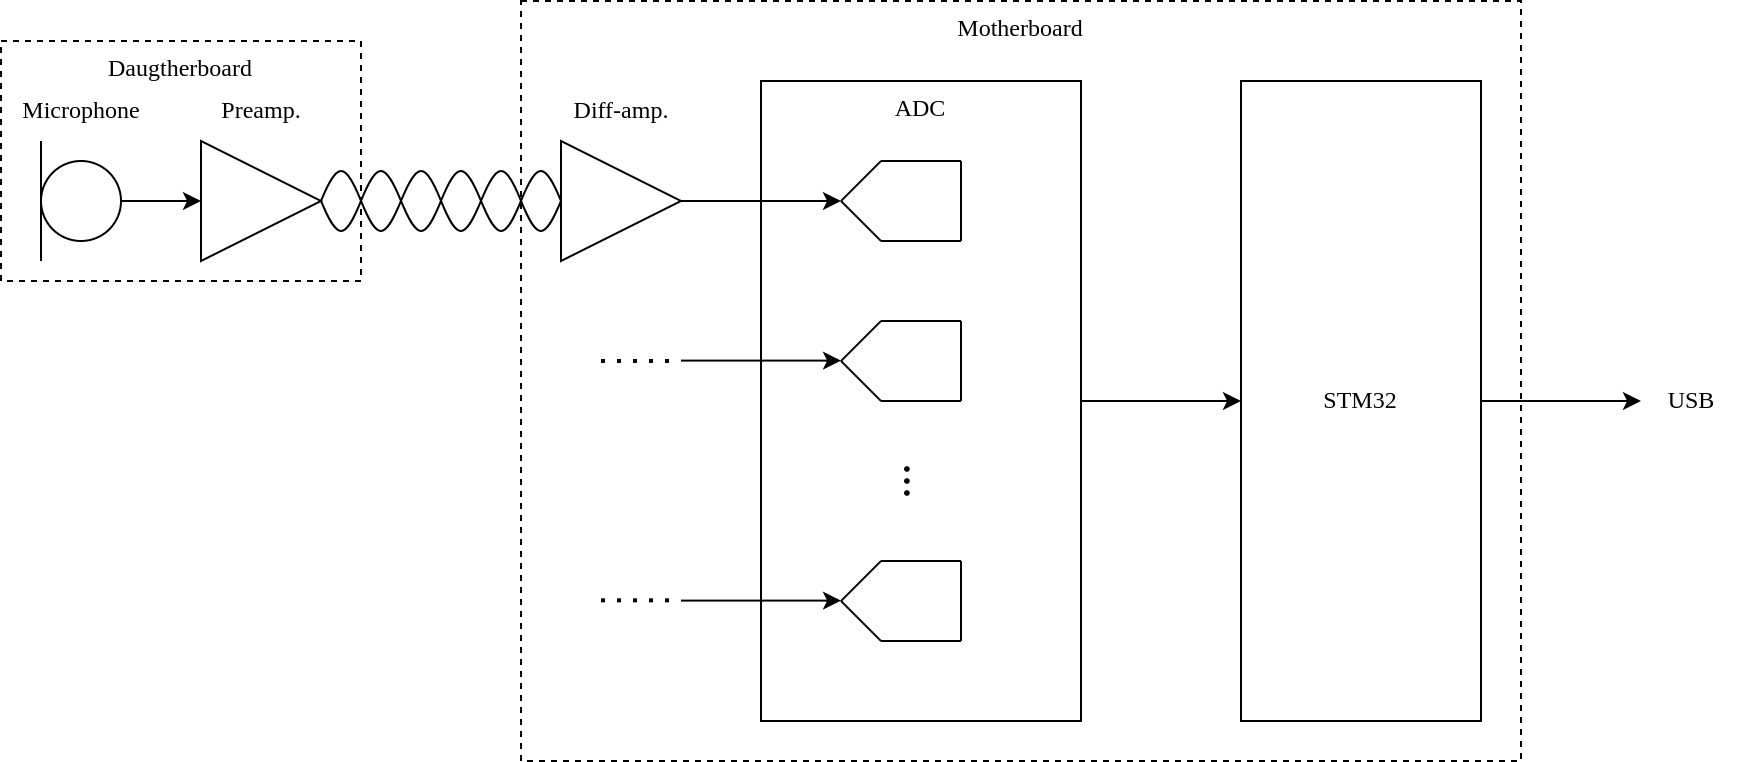
\includegraphics[width=0.9\textwidth]{./design_overall.png}
\centering
\caption{The overall electronics-design with only one daughterboard as an example.}
\label{fig:design_overall}
\centering
\end{figure}

%\tikzstyle{block} = [
%	draw, 
%	rectangle, 
%	minimum height = 0.5cm, 
%	minimum width = 0.5cm
%]
%\tikzstyle{output} = [
%	coordinate
%]
%
%\begin{figure}[H]
%\begin{tikzpicture}[auto, node distance=2cm]
%	\node [block, label=Mic.] (mic0) {};
%	\node [block, right of=mic0, label=Preamp.] (preamp0) {};
%	\node [block, right of=preamp0, label=Diff.-Amp.] (diffamp0) {};
%	
%	\draw [->] (mic0) -- (preamp0);
%	\draw [->] (preamp0) -- (diffamp0);
%	
%%	\node [block, right of=diffamp0, minimum height=2cm] (adc) {ADC};
%%	\node [block, right of=adc, minimum height=2cm] (stm32) {STM32};
%%	
%%	\draw [->] (diffamp0) -- (adc);
%%	\draw [->] (adc) -- (stm32);
%\end{tikzpicture}
%\centering
%\caption{The sequence of triggers for the hardware timers in the STM32.}
%\label{fig:design_overall}
%\centering
%\end{figure}

\subsection{Filtering and Sampling}

Given that the ADC already had anti-aliasing filters, then the channels must have been sampled to give enough oversampling. From the ADC's datasheet, the filters had a gentle roll-off of -20 \si{dB/dec} and a cut-off frequency at -3 \si{dB} of about 15 \si{kHz} \cite{noauthor_8-channel_2021}. Therefore, each channel was sampled eightfold than the decimated sampling frequency\footnote{The reader must keep in mind that there are two sampling frequencies; one is the physical sampling of the ADC, and the other is sampling frequency of the discrete digitally decimated signal in the firmware. The former is much higher than the latter, and the latter corresponds to the same discrete sampling frequency discussed in Chapter-\ref{Simulation_of_the_Proposed_System} on the simulations, etc.}, i.e. 24 \si{kHz}, such that the Nyquist frequency is eightfold the bandwidth of interest, i.e. 12 \si{kHz}. The folded aliases were thus attenuated around -20 \si{dB} as seen in Figure-\ref{fig:design_spectrum}.

\begin{figure}[H]
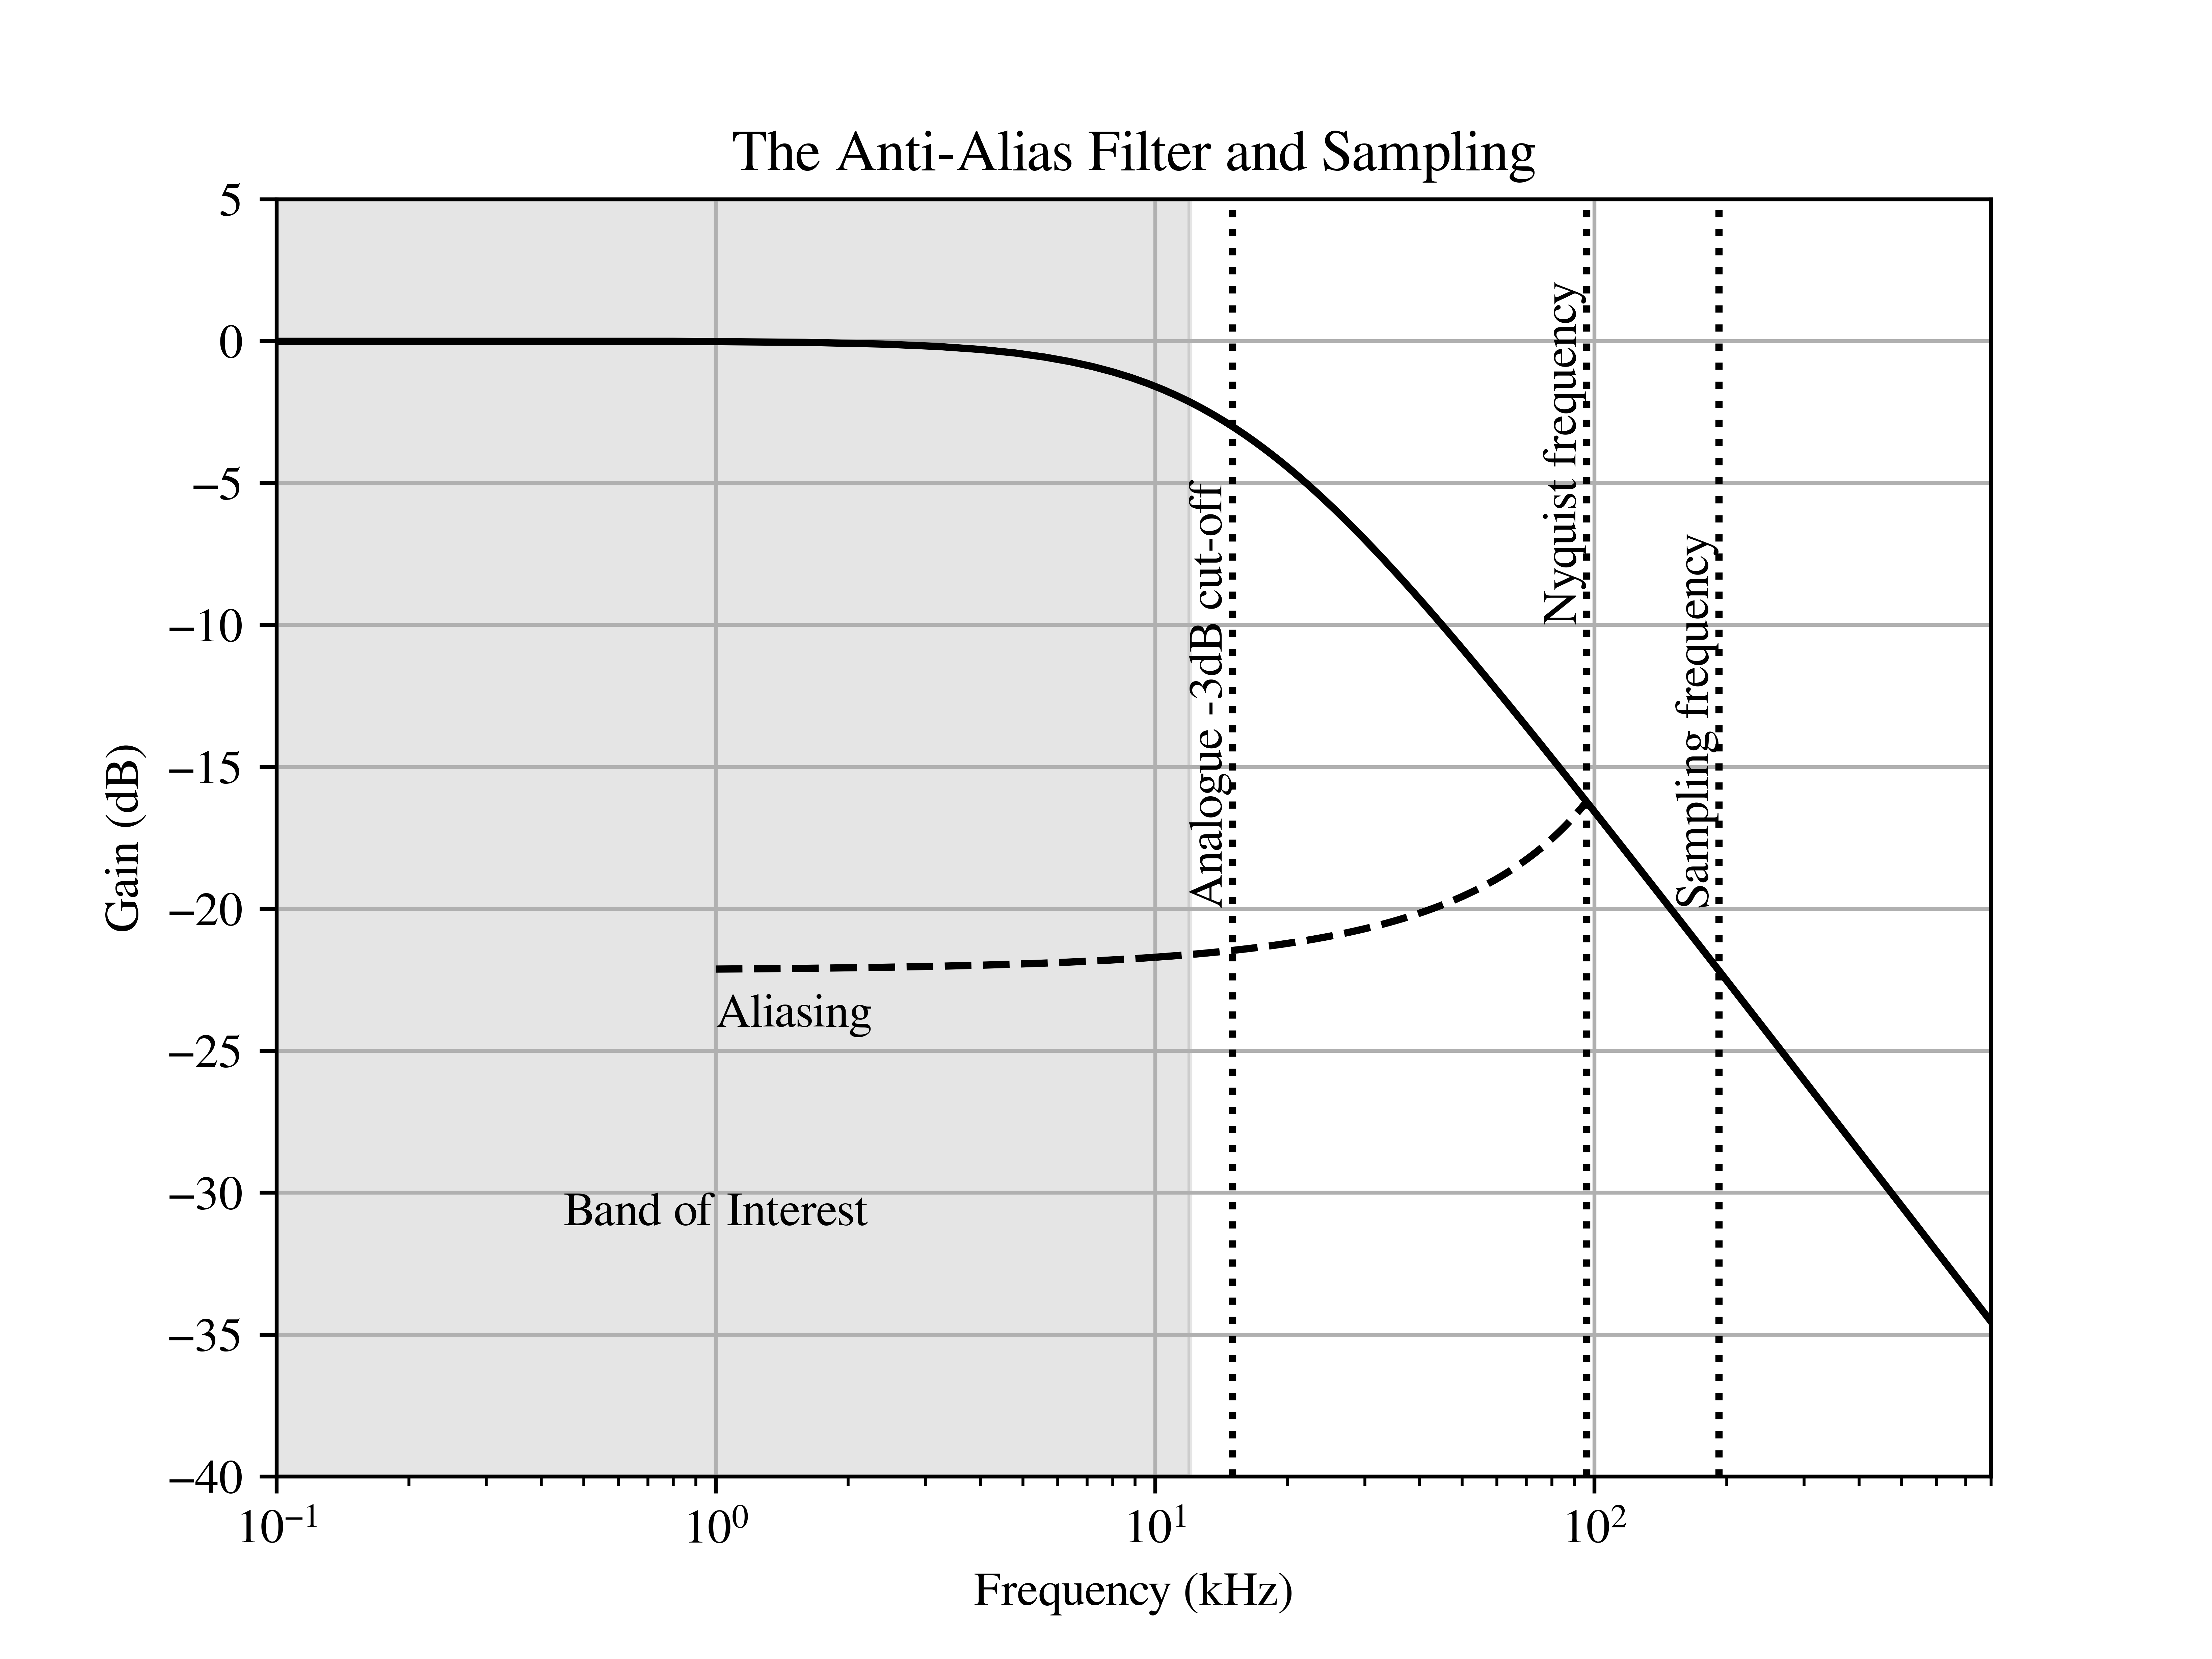
\includegraphics[width=0.9\textwidth]{../Python/report/spectrum.png}
\centering
\caption{The analogue anti-alias filter and the sampled spectrum after the ADC.}
\label{fig:design_spectrum}
\centering
\end{figure}

\subsection{Dynamic Range}

Given all of the analogue components, a chain of signals and gains could be designed. First, the microphone has a sensitivity of -38 \si{dBV} at a level of 94 \si{dB_{SPL}}. For this system, 90 \si{dB_{SPL}} was taken as the highest level. This would translate to an output voltage of $-38 + 90 - 94 = -42 \si{dBV}$ or 7.94 \si{mV}. Given a 68 \si{\Omega} gain-selecting resistor, the gain of the preamplifier was empircally found to be 33 \si{dB}\footnote{This is depsite the datasheet saying 40 \si{dB}}. Therefore, the differential signal across the twisted pair was:
\begin{equation}
-42 + 33 = -9 \si{dBV} \text{ or } 355 \si{mV}
\end{equation}
in amplitude.

As seen in Figure-\ref{fig:design_gains}, the microphone's noise-floor is given by its SNR and lies at a sound-level of 29 \si{dB_{SPL}} of the leftmost axis. On the second axis on the left is the microphone's voltage corresponding to such sound-level. This is amplified by 33 \si{dB} by the preamplifier which gives the third axis in the middle.

\begin{figure}[H]
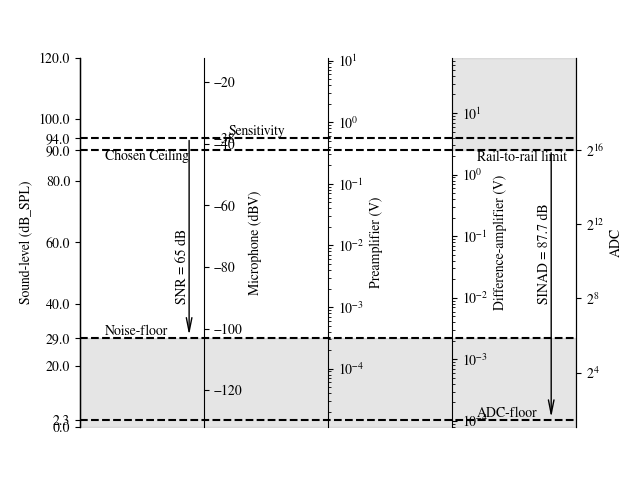
\includegraphics[width=0.9\textwidth]{../Python/report/gains.png}
\centering
\caption{The levels of the signal for each stage in the signal-path.}
\label{fig:design_gains}
\centering
\end{figure}

Therefore, to bring this to the rail-to-rail range of the difference-amplifier which was $\pm2.5 \si{V}$, its gain must have been:
\begin{equation}
G_{\text{diff.}} = \frac{2.5 \si{V}}{355 \si{mV}} = 7.05 \text{ or } 17 \si{dB}
\end{equation}

The difference-amplifier's gain was set using 2.0 \si{k\Omega} and 15.0 \si{k\Omega} resistors which were chosen to have low resistances to reduce the thermal Johnson noise.

Thus, as seen in Figure-\ref{fig:design_gains}, the chosen limit of 90 \si{db_{SPL}} corresponds roughly with the difference-amplifier's 2.5 \si{V} rail. Since the ADC is defaulted to a range $\pm5 \si{V}$, this is half the ADC's full-scale which only reduces the SINAD by 6 \si{dB}. Given the ADC's SINAD, the ADC's effective floor corresponds with 8.3 \si{dB_{SPL}} on the leftmost axis which is a good 20.7 \si{dB} below the noise-floor.

\section{Printed Circuit-Boards}

\subsection{Motherboard}

A PCB was needed so that EMI could be mitigated and so that the prototype was neat and tidy and could fit inside the NUgus' head. The use of ground-planes is a common way to shield EMI. Also, it allows return-currents of fast signals to flow along the path of least impedance. This shrinks the area between the signal and the return-current so that it behaves less as an antenna.

\subsubsection{Layers}

The PCB was chosen to have four layers because of the design's complexity. The stack-up of layers was such:

\begin{table}[H]
\caption{The motherboard's stack-up of layers.}
\label{tab:pcb_layers}
\centering
\begin{tabular}{c}
	\hline
	Signals \\
	\hline
	Ground \\
	\hline
	Power and Ground \\
	\hline
	Jumpers \\
	\hline
\end{tabular}
\centering
\end{table}

This allowed supply-voltages like 5 \si{V} and 3.3 \si{V} to be routed under all the components and signals since these supply-voltages were often needed in many places. It also allowed the bottom layer to be used for jumping signals underneath other signals and components while at the same time keeping a solid ground-plane as top inner layer. Thus, two layers would not have been possible without having signals jumping across the ground-plane on the bottom layer.

Such as design is seen in Figure-\ref{fig:design_pcb_mother}.

\begin{figure}[H]
\begin{subfigure}{0.5\textwidth}
	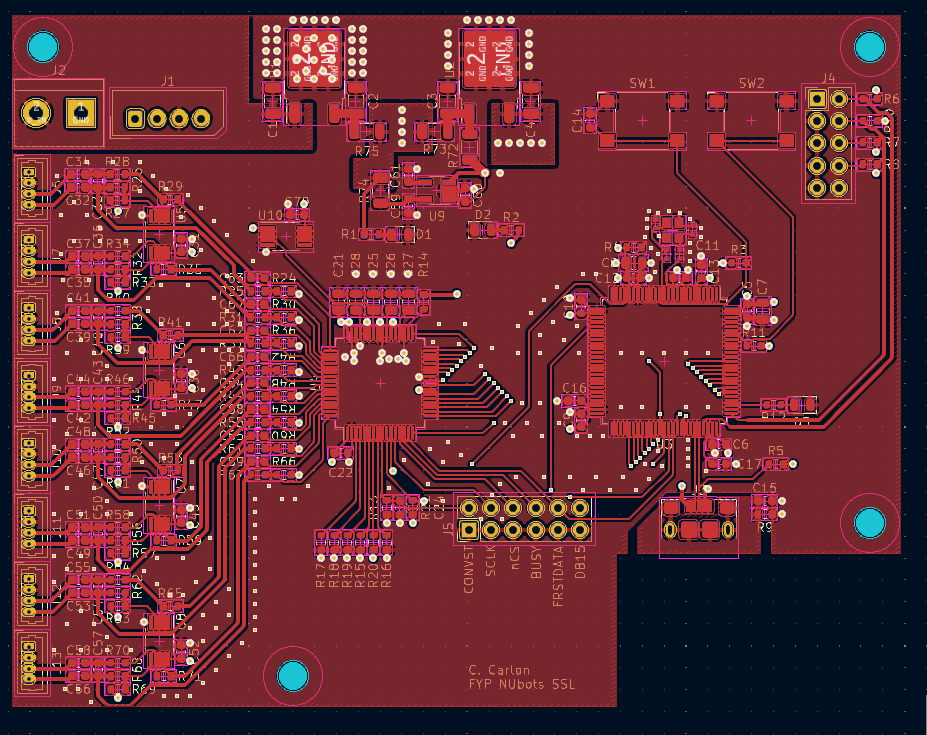
\includegraphics[width=.9\textwidth]{./pcb/mother/top.png}
	\centering
	\caption{top}
	\label{fig:design_pcb_mother_top}
	\centering
\end{subfigure}
\begin{subfigure}{0.5\textwidth}
	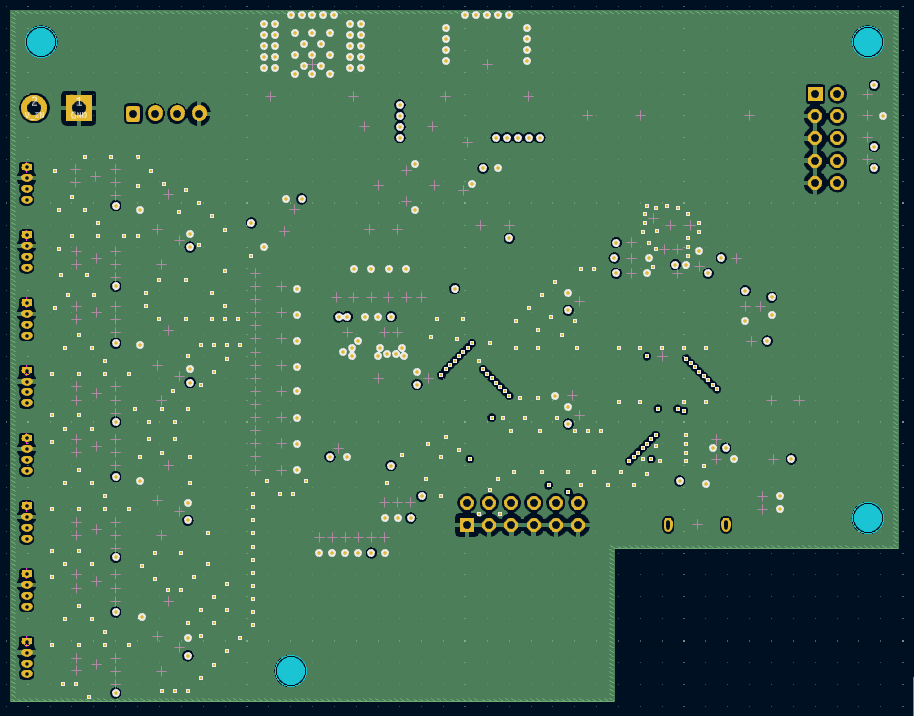
\includegraphics[width=.9\textwidth]{./pcb/mother/first_inner.png}
	\centering
	\caption{first inner}
	\label{fig:design_pcb_mother_first}
	\centering
\end{subfigure}
\begin{subfigure}{0.5\textwidth}
	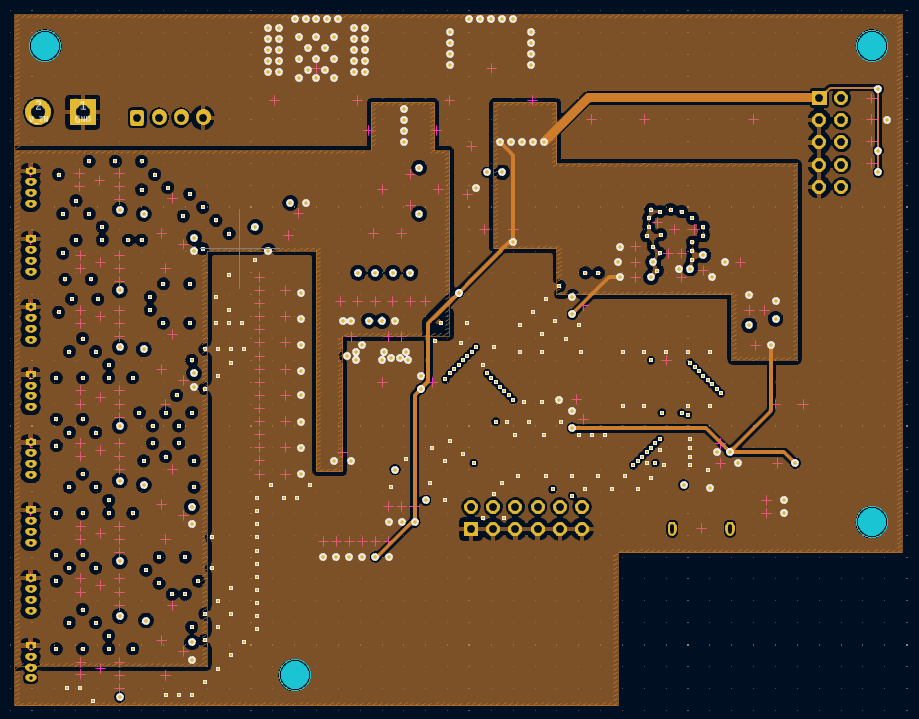
\includegraphics[width=.9\textwidth]{./pcb/mother/second_inner.png}
	\centering
	\caption{second inner}
	\label{fig:design_pcb_mother_second}
	\centering
\end{subfigure}
\begin{subfigure}{0.5\textwidth}
	\includegraphics[width=.9\textwidth]{./pcb/mother/bottom.png}
	\centering
	\caption{bottom}
	\label{fig:design_pcb_mother_bottom}
	\centering
\end{subfigure}
\caption{The layers of the motherboard. a: top. b: first inner. c: second inner. d: bottom.}
\label{fig:design_pcb_mother}
\centering
\end{figure}

%\subsubsection{Return-paths}
%
%Signals of high frequency tend to have return-currents that flow in a thin symmetric path on the ground-plane directly beneath (or above). Although there was no RF circuitry with high frequencies, careful attention was needed for high frequency with the digital circuitry.
%
%In particular, careful attention was given the ground-plane directly above the jumping digital data-lines for the parallel interface. Although this layer was for both power and ground, no power lines were routed across this area so that return-currents had a straight path.
%
%Given that there were sensitive analogue circuitry such as the ADC itself, the PCB was split up into two areas, one digital and the other analogue. Furthermore, the analogue circuitry took 5 \si{V} whereas the digital circuitry elsewhere took 3.3 \si{V}. Thus, the two linear regulators for each voltage were put such that the return-currents for the ADC and the STM32 did not cross.
%
%\subsubsection{Stitching and Shielding Vias}
%
%When a fast signal changed layer, a stitching via was needed to bypass the return-current to ground plane on the other side of the core to give less impedance and to shrink the loop's area.
%
%Shielding vias were added around sensitive signals such as the analogue differntial pairs and around noisy signals such as the clock signal to the ADC.
%
%\subsubsection{Propogation-delay}
%
%The digital data-lines for the parallel interface were made to have similar lengths such that the relative propogation-delay was little. If this was to much for example, then the bits may be out by a few clock-cycles, and the data would be scrambled.

\subsection{Daughterboard}

Given that the array was a cube about 80 \si{mm} wide, each microphone was going to be away from the board. Also, given that the microphone needed to be preamplified as near as possible to the microphone itself and sent as a differential signal along a twisted pair, each microphone needed its own PCB for the circuitry. Thus, each microphone needed its own daughterboard.

Unlike the motherboard, each daughterboard had two layers because of the relative simplicity.

\begin{figure}[H]
\begin{subfigure}{0.5\textwidth}
	\includegraphics[width=.9\textwidth]{./pcb/daughter/top.png}
	\centering
	\caption{top}
	\label{fig:design_pcb_daughter_top}
	\centering
\end{subfigure}
\begin{subfigure}{0.5\textwidth}
	\includegraphics[width=.9\textwidth]{./pcb/daughter/bottom.png}
	\centering
	\caption{bottom}
	\label{fig:design_pcb_daughter_bottom}
	\centering
\end{subfigure}
\caption{The layers of the daughterboard. a: top. b: bottom.}
\label{fig:design_pcb_daughter}
\centering
\end{figure}

Physically, the PCB directly around the microphone was made to be small as seen in Figure-\ref{fig:design_pcb_daughter} so that the sound-waves had less path of flight to the microphone's port. Although the large area of PCB may still hinder the path of flight, it could be helped.

Furthermore, a hole was added so that each daughterboard could be easily attached to a frame.

\chapter{Firmware Design}

With the electronics designed, the firmware had to be designed to apply the sound-source-localisation algorithm. Again, this area was particularly important to this project especially given its novelty since not many examples were done on an embedded system. Thus, this chapter hereafter talks about the functions used. 

No raw code is given to keep this report short, but one can visit the GitHub repository which has all code used in this project\footnote{Note that there may be commits afterwards.}: \url{https://github.com/Claegtun/fyp-nubots-ssl}.

\section{Overall Design}

The first few operations of the firmware were the pre-processing before the computation of the GCC-PHATs and then the energy-map as seen in Figure-\ref{fig:firmware_overall}. Since the ADC outputs each channel sequentially for each sample-period, then the buffer of data from it has to deinterleaved into eight individual vectors for each channel. Next, this oversampled data has to be digitally filtered and then decimated to a chosen sampling frequency. This was done in one function, see Section-\ref{Digital_Filter}. Afterwards, this data was still in 16-bit format and had to be converted to floating-point data. Then, the FFT of the decimated time-domain data was computed along with its complex magnitude and complex conjugate. These were then used to compute the GCC-PHAT for each pair of microphones. Afterwards, the energy-map was drawn from this.

\tikzstyle{block} = [
	draw, 
	rectangle, 
	minimum height = 1cm, 
	minimum width = 1cm
]
\tikzstyle{input} = [
	coordinate
]

\begin{figure}[H]
\begin{tikzpicture}[auto, node distance=2cm]
	\node [input, name=input] {};
	\node [block, right of=input] (deint) {Deinterleaving};
	\node [block, right=1cm of deint] (dec) {Decimation};
	\node [block, right=1cm of dec, align=center] (float) {Conversion to\\ Floating-point};
	\node [block, below of=dec] (fft) {FFT};
	\node [block, right of=fft] (mag) {Magnitude};
	\node [block, left of=fft] (conj) {Conjugate};
	
	\node [block, below of=fft, minimum width=8cm] (gcc) {GCC-PHAT};
	
	\node [block, below of=gcc] (beam) {Energy-map};
	
	\node [above=0.5cm of fft] (mid) {};
	
	\draw [->] (input) -- (deint);
	\draw [->] (deint) -- (dec);
	\draw [->] (dec) -- (float);
	\draw [-] (float.south) |- (mid.south);
	\draw [->] (mid.south) -- (fft);
	\draw [->] (fft) -- (mag);
	\draw [->] (fft) -- (conj);
	
	\draw [->] (fft) edge (gcc.north -| fft);
	\draw [->] (mag) edge (gcc.north -| mag);
	\draw [->] (conj) edge (gcc.north -| conj);
	
	\draw [->] (gcc) -- (beam);
\end{tikzpicture}
\centering
\caption{The overall design of the firmware.}
\label{fig:firmware_overall}
\centering
\end{figure}

\section{Parallel Interface}

The ADC could communicate through either a serial or a parallel interface. After some testing with an development-board of the ADC and a STM32 Nucleo board, it was found that the parallel interface was more reliable. Since the parallel interface has sixteen data-lines for each bit of the ADC result, the datalines were connected to pins common to one of the GPIO ports, namely Port-E.

Given that the system would ideally be real-time, a single frame of data from the ADC had to be gotten through DMA without any CPU instructions between each sample. The STM32 allows a GPIO-port's IDR to be transferred by DMA to a buffer.

The ADC took a CONVST signal on the rising edge of which would trigger a conversion of all eight channels \cite{noauthor_8-channel_2021}. Thus, this signal had to be generated by a hardware-timer. Furthermore, a nCS signal was needed to go low for each lot of samples from all eight channels. Finally, the ADC needed an nRD signal to pulse eightfold and to thus gate each channel, similar to a serial clock. These signals had to be timed and linked together. 

%The parameters for such timers are given in Table-\ref{tab:timers}.
%
%\begin{table}[H]
%\caption{The timers' parameters set for the ADC's parallel interface given a peripheral clock-frequency of 275 \si{MHz}.}
%\label{tab:timers}
%\centering
%\begin{tabular}{c c c c c c c}
%	\hline
%	Signal	& Timer	& ARR	& CRR1	& RCR	& Period (ns)	& Pulse-width (ns) \\
%	\hline
%	\hline
%	CONVST	& TIM2	& 572	& 247	&		& 2080			& 898 \\
%	\hline
%	nCS		& TIM3	& 479	& 1		&		& 1750			& 3.64 \\
%	\hline
%	nRD		& TIM8	& 53		& 40		& 7		& 196			& 145 \\
%	\hline
%			& TIM4	& 2		&		&		& 10.9			&	\\
%	\hline
%			& TIM5	& 17		& 13		&		& 65.5			& 47.3 \\
%	\hline
%\end{tabular}
%\centering
%\end{table}
%
%The timer for the CONVST signal TIM2 was chosen to have a period of 2.08 \si{\micro s} so that the conversions were done at a sampling frequency of 480 \si{kHz}. 
%
%The timer for the nCS signal TIM3 was chosen to have a short high pulse so that the rest of the period was low; the period was chosen to be long enough for the data of all eight channels. 
%
%The timer for the nRD signal TIM8 was set to have eight repeated pulses, one for each channel.
%
%The two other timers TIM4 and TIM5 had no outputs but rather were for timing the firmware. TIM4 was used to trigger TIM8 10 \si{ns} after the output of TIM3 went low. This was since the ADC's datasheet specifies that the nRD signal must go low after the nCS goes low.
%
%TIM5 was used to trigger the DMA transfer of Port-E's IDR. It was triggered by TIM8 and had a pulse 47.3 \si{ns} wide so that the transfer was roughly in the middle of the low nRD pulse.
%
%Each timer has a specific set of other available timers to be triggered therefrom. For example, TIM8 can be triggered by TIM2 but not TIM3. Therefore, according to Table-350 and -355 in the reference-manual, the timers were chosen so that the following sequence in Figure-\ref{fig:firmware_timers} could be made \cite{noauthor_stm32h723733_2021}.
%
%\tikzstyle{block} = [
%	draw, 
%	rectangle, 
%	minimum height = 1cm, 
%	minimum width = 2cm
%]
%\tikzstyle{output} = [
%	coordinate
%]
%
%\begin{figure}[H]
%\begin{tikzpicture}[auto, node distance=3cm]
%	\node [block] (tim2) {TIM2};
%	\node [block, right of=tim2] (tim3) {TIM3};
%	\node [block, below of=tim3] (tim4) {TIM4};
%	\node [block, right of=tim4] (tim8) {TIM8};
%	\node [block, right of=tim8] (tim5) {TIM5};
%	
%	\draw [->] (tim2) -- (tim3);
%	\draw [->] (tim2) -- (tim4);
%	\draw [->] (tim4) -- (tim8);
%	\draw [->] (tim8) -- (tim5);
%\end{tikzpicture}
%\centering
%\caption{The sequence of triggers for the hardware timers in the STM32.}
%\label{fig:firmware_timers}
%\centering
%\end{figure}

\section{Digital Filter} \label{Digital_Filter}

In order to decimate the oversampled signal from the ADC, it must first have been filtered with a steep roll-off lest there were aliases from the decimation. This was since decimating is akin to further sampling in discrete time. The steeper the roll-off the better kept the band of interest is. Ideally, both cut-off at -3 \si{dB} and that at -20 \si{dB} would lie around the bandwidth of interest which was in this case 12 \si{kHz} since the chosen decimated sampling frequency was 24 \si{kHz}.

However, care was taken with the number of taps, i.e. the order, lest the computation took too long. A FIR filter was used since it is computationally lighter. It was found that 128 taps was enough to get a reasonably steep roll-off where the cut-off at -3 \si{dB} lied around 10 \si{kHz} and that at -20 \si{dB} cut-off lied around 13 \si{kHz}. This would ensure that most aliases were attenunated by -20 \si{dB} and that the workable bandwidth was 10 \si{kHz} which is 83 \% of the Nyquist frequency of 12 \si{kHz}, i.e. the chosen bandwidth of interest.

\begin{figure}[H]
\includegraphics[width=0.9\textwidth]{../Python/filter/frequency.png}
\centering
\caption{The frequency-response of the digital filter before decimation.}
\label{fig:filter_frequency}
\centering
\end{figure}

The ARM Cortex-M7 CPU has a number of SIMD instructions for multiplication and accumulative addition that can be run in a single instruction-cycle\cite{noauthor_digital_2018}. Furthermore, CMSIS has a DSP library for many of the ARM Cortex-M processors; in which are a few functions specially for fitlering and decimating. In this project, the function that was used was \texttt{arm\_fir\_decimate\_q15} which takes a pointer to a block $DF$ samples long and computes a block $F$ samples long where $F$ is the decimated block's length, $D$ is the decimation-factor.

This function takes up the CPU and as such affects the overall computational and real-time performance of the system. One alternative to filtering is the STM32's FMAC which can offload filter-operations from the CPU and read data from a buffer in memory\cite{noauthor_stm32h723733_2021}. This quicker alternative may be looked thereinto later for the demonstration-day.

\section{FFT and Other Mathematical Functions}

The SRP algorithm relies a lot on the Fourier transform, namely FFT. As such, it was needed to optimise the FFT as much as possible. As said before, the ARM Cortex-M7 CPU has a few hardware-accelerated instructions and a DSP library from CMSIS. Thus, there are a few optimised FFT functions.

One such function that was used was \texttt{arm\_rfft\_fast\_f32} which takes a pointer to a block of real samples and computes a block of complex values twice as long; it also computes the real inverse given a block of complex values. This function in particular is somewhat faster and takes advantage of symmetry since the input data is real. Some other functions are written down in Table-\ref{tab:dsp_functions}.

\begin{table}[H]
\caption{Other mathematical functions used from the CMSIS DSP library.}
\label{tab:dsp_functions}
\centering
\begin{tabular}{p{0.4\textwidth} p{0.5\textwidth}}
	\hline
	Function							& Description	\\
	\hline
	\hline
	\texttt{arm\_cmplx\_mag\_f32}	
	& Computes the complex magnitudes of an array of complex numbers. \\
	\hline
	\texttt{arm\_cmplx\_conj\_f32}
	& Computes the complex conjugate of an array of complex numbers. \\
	\hline
	\texttt{arm\_mult\_f32}
	& Computes the dot-product of two arrays as vectors. \\
	\hline
	\texttt{arm\_cmplx\_mult\_cmplx\_f32}
	& Computes the product of each pair of complex numbers with two arrays. \\
	\hline
\end{tabular}
\centering
\end{table}

From the proposed algorithm in Algorithm-\ref{alg:proposed_algorithm}, a number of optimisations had been made, such as computing each channel's FFT, its magnitue, and its conjugate once before computing the GCC-PHAT many times for many different pairs. This was better than needlessly computing each of these values many times within the same loop for computing the GCC-PHAT. These values could instead be computed once for each channel and then passed by pointers to the function that computes the GCC-PHAT.

\chapter{Testing}

Although the prototype was not done in time for thorough physical experiments, most of the functionality was working. Thus, this chapter shows the basic promising functionality so that the prototype is fully working on the demonstration-day.

%\section{Electronics}
%
%\subsection{Analogue Signal-path}
%
%After the physical electronics was assembled, the signal-path from the microphone to the ADC was tested. As seen in Figure-\ref{fig:testing_signal}, the preamplifier's signal has an amplitude of 93 \si{mV}. This signal is then amplified again by the difference-amplifier on the motherboard by a gain of 7 which gives an amplitude of 2.57 \si{V}. As seen in , the analogue circuitry works fairly well.
%
%\begin{figure}[H]
%\includegraphics[width=0.9\textwidth]{./testing_signal.png}
%\centering
%\caption{The output of the preamplifier (yellow) and that of the difference-amplifier (green).}
%\label{fig:testing_signal}
%\centering
%\end{figure}

\section{Firmware}

\subsection{Computation and Timing} \label{Computation_and_Timing}

To make sure that the system can run in real-time, each step of the algorithm and the firmware was timed on a single frame. This was done with a Saleae Logic Analyser. As seen in Figure-\ref{fig:testing_timing}, the longest operation was drawing the energy-map. This was since there is 2562 directions along which to compute the energy.

\begin{figure}[H]
\includegraphics[width=0.9\textwidth]{./results_timing.png}
\centering
\caption{The timing of the computation given a single frame of data where "0" is time taken to deinterleave the data from the ADC, "1" to decimate the oversampled signal with a digital filter and to convert it to floating-point values, "2" to compute the FFT, its magnitude, and its conjugate, "3" to compute the GCC-PHAT for all pairs, and "4" to draw the energy-map and to find the estimated direction.}
\label{fig:testing_timing}
\centering
\end{figure}

Overall, the whole computation generally takes about 43 \si{ms}. This is roughly equal to the frame's period of:
\begin{equation}
T_F = \frac{1024}{f_s} = \frac{1024}{24 \si{kHz}} = 42.7 \si{ms}
\end{equation}
Thus, given two buffers where one is being filled by the ADC, and the other is being processed, the system can run in real-time. However, there is not much more that can be done after estimating the basic direction. A more sophisticated digital filter for decimation may be needed to improve the time for computation as talked about in Section-\ref{Digital_Filter}. This will be needed to also include an extended Kalman filter (EKF) as an extension.

\subsection{Signal-processing}

From Figure-\ref{fig:testing_fft}, the FFT worked reasonably well as it showed a peak around 1 \si{kHz} when a tone of that frequency was played nearby. This shows that most of the signal-path and the firmware until this point works reasonably well.

\begin{figure}[H]
\includegraphics[width=0.9\textwidth]{../Python/main_method/physical/fft.png}
\centering
\caption{An example of the FFT done on one microphone's signal, i.e. channel with a 1 \si{kHz} tone playing nearby.}
\label{fig:testing_fft}
\centering
\end{figure}

\subsection{Preliminary Energy-map}

Although some further work is needed, an energy-map using the SRP-PHAT algorithm was drawn when a very fast metronome was played nearby, emulating impulses. As seen in Figure-\ref{fig:testing_map}, a peak is seen roughly where the sound was. Indeed, further testing is needed before the demonstration-day as discussed in Chapter-\ref{Physical_Experiments}.

\begin{figure}[H]
\includegraphics[width=0.9\textwidth]{../Python/main_method/physical/map.png}
\centering
\caption{An energy-map drawn by an early version of the localisation-algorithm.}
\label{fig:testing_map}
\centering
\end{figure}

\chapter{Physical Experiments} \label{Physical_Experiments}

Although the basic functionality of the prototype was done, there was not enough time to do any physical experiments in time for this report. However, this chapter has the methodology to be done afterwards.

\section{Experimental Set-up}

For all experiments, the prototype, i.e. the microphone-array, will be set in the middle of an empty, most likely the NUbots field which is about 4 \si{m} wide, 6 \si{m} long, and 3 \si{m} high. It also has field of artificial grass that takes up most of the room and mitigates reverberation like carpet. This will give the most realistic and intentional environment to test in.

The array will be set on a tripod 1 \si{m} tall. This height will emulate the height of a NUgus robot. The speaker playing the recording will also be on another tripod that is also 1 \si{m} tall. Each tripod will also have a plumb-bob dangling to the ground so that the distance can be accurately measured. 

\section{Effect of Distance}

Emulating the SNR directly is hard since it is difficult to control the thermal noise and the environmental noise given a signal. However, the signal's intensity is proportional to the inverse of the squared distance. Therefore, a correlative trend can be gotten by varying the distance while the intensity at the source is kept constant.

However, the distance also affects the accuracy when the source is near the array since the algorithm relies on the far-field approximation, see Section-\ref{The_far_Field_and_the_near_Field}. Either way, this should emulate the simulations in Section-\ref{Performance_against_Noise}.

\subsection{Experimental Method}

A recording of claps will be played at distances varying from 1 to 3 \si{m} in intervals of 0.5 \si{m}. Ten plays of the recording are to be done for each distance.

\section{Effect of Angle}

A variable that has not been tested much in the simulations is the angle. This is important for the physical prototype since there may be unforeseen discrepencies in the electronics, etc.

\subsection{Experimental Method}

A recording of claps will be played 2 \si{m} away from the source at azimuths varying in intervals of 45 \si{\degree}. Only the azimuth is varied because of the space. Ten plays of the recording are to be done for each azimuth.

\section{Effect of Type}

The simulations have looked into the difference in performance between a broadband signal, namely a clap, and a narrowband signal, namely a whistle. The latter is especially important to test for the physical prototype since it is the worse. This experiment will also help evaluate the effect of the estimated confidence and the threshold which is to forsake spurious estimated directions in the middle of a whistle.

\subsection{Experimental Method}

Since the distance was already tested with a recording of claps, the same experiment was done with a recording of a whistle's burst. Like before, it will be played at distances varying from 1 to 3 \si{m} in intervals of 0.5 \si{m}. Ten plays of the recording are to be done for each distance.

\chapter{Post-processing}

After the algorithm has computed an estimated direction along with an estimated confidence, then it needs to be processed by a human for testing and demonstration. The most basic way is to send the results as ASCII over the USB-connection.

\section{Extended Kalman Filter}

An additional process to be added would be an extended Kalman filter (EKF) to smooth the estimated direction over many temporal ones straight from the SRP algorithm.

\section{Visualisation}

One more task to do after the report and before the demonstration-day is some kind visual post-processing to help demonstrate and the performance of the system. There are a few ways to do this:
\begin{itemize}
	\item to generate a three-dimensional scene with an estimated direction as a line or cone given the confidence,
	\item to make the robot's head turn towards the estimated direction,
	\item or to use the NUbots visual tool called NUsight to overlay the estimated direction over a live camera-feed.
\end{itemize}

The second of which may need an EKF since the robot needs smooth motions. The last of which may be fairly complex since the NUsight environment is not very flexible and is developed in Typescript which is a web-based language.

\chapter{Conclusion}

\section{Progress}

So far, a basic physical prototype has been made, and on which, the sound-source-localisation algorithm, namely SRP-PHAT, seems to work. All of the electronics has been done and works reasonably well although some more testing and tuning may be needed.

Furthermore, a thorough set of simulations have been done on both two literature-examples and the proposed design.

\section{Findings}

It has been found that the SRP-PHAT method for sound-source-localisation is feasible on a small embedded application. However, constraints such as the sampling frequency have a heavy weight on the performance. It was also found in Section-\ref{Effect_of_Delay} that the robot's head being a solid object may affect the performance.

\section{Future Work}

In the short term before the demonstration-day, further tuning and troubleshooting of the firmware is needed. The burden of computation especially needs to be lessen so that more post-processing can be done real-time; this may be done by offloaded the digital fitler, see Section-\ref{Digital_Filter}. Afterwards, thorough physical experiments are needed to test the performance and the robustness, see Chapter-\ref{Physical_Experiments}. Also, a post-processing technique is needed to help give a visual guide for spectators on demonstration-day.

In the long term, much further research is needed into more novel and sophisticated techniques of sounbd-source-localisation while at the same time keeping the embedded aspect in mind. For example, a technique that can estimate distance would be highly sought after. Furthermore, different kinds of methods may be looked into such as binaural ones which only use two microphones or ones that use machine-learning.

%\nocite{*}

\bibliographystyle{plain}
\bibliography{./zotero}

\begin{appendices}
\chapter{Schematics of Electronics} \label{Schematics_of_Electronics}
\includepdf[pages=-,pagecommand={},angle=90,width=1.4\textwidth]{schematics.pdf}
\end{appendices}

%\includepdf[pages=-,pagecommand={},angle=90,width=\textwidth]{controller_1.pdf}

%\begin{figure}[!h]
%\includegraphics[width=0.9\textwidth]{image.png}
%\centering
%\caption{Caption,}
%\label{fig:image}
%\centering
%\end{figure}

%\includepdf[pages=-,pagecommand={},angle=90,width=\textwidth]{controller_1.pdf}
%\includepdf[pages=-,pagecommand={},angle=90,width=\textwidth]{regulator_1.pdf}
%\includepdf[pages=-,pagecommand={},angle=90,width=\textwidth]{timer_1.pdf}


\end{document}
